%
% uaThesis example (for a thesis written in Portuguese)
%
% the complete list of options and commands can be found in uaThesis.sty 
%

\documentclass[11pt,twoside,a4paper]{report}
\usepackage[DETI,newLogo,final]{uaThesis}


\usepackage[T1]{fontenc}
\usepackage{subcaption}
\usepackage[utf8]{inputenc}

%Francisco
\usepackage{amsmath}
\usepackage{float}
\usepackage{url}
\usepackage{hyperref}




\newenvironment{spmatrix}[1]
 {\def\mysubscript{#1}\mathop\bgroup\begin{pmatrix}}
 {\end{pmatrix}\egroup_{\textstyle\mathstrut\mysubscript}}

\usepackage[dvipsnames]{xcolor}

\usepackage{fancyvrb}

% redefine \VerbatimInput
\RecustomVerbatimCommand{\VerbatimInput}{VerbatimInput}%
{fontsize=\footnotesize,
 %
 frame=lines,  % top and bottom rule only
 framesep=2em, % separation between frame and text
 rulecolor=\color{Gray},
 %
 label=\fbox{\color{Black}ffserver.conf},
 labelposition=topline,
 %
 commandchars=\|\(\), % escape character and argument delimiters for
                      % commands within the verbatim
 commentchar=*        % comment character
}


\def\ThesisYear{2019}

% optional packages
%\usepackage[portuguese]{babel}
\usepackage[english]{babel}
%\usepackage[latin1]{inputenc}
\usepackage{hyperref}
\usepackage{amsmath}
\usepackage{amssymb}
\usepackage{xspace}% used by \sigla
%\usepackage[newcentury]{quotchap}
\usepackage[printonlyused]{acronym}
%\usepackage{acronym}
\usepackage{underscore}
\usepackage[noend]{algpseudocode}
\usepackage{algorithm}
%\usepackage{parskip}

\usepackage{float}
% optional (comment to use default)s
%   depth of the table of contents
%     1 ... chapther and sections
%     2 ... chapters, sections, and subsections
%     3 ... chapters, sections, subsections, and subsubsections
\setcounter{tocdepth}{3}
\setcounter{secnumdepth}{4}
% optional (comment to used default)
%   horizontal line to separate floats (figures and tables) from text
\def\topfigrule{\kern 7.8pt \hrule width\textwidth\kern -8.2pt\relax}
\def\dblfigrule{\kern 7.8pt \hrule width\textwidth\kern -8.2pt\relax}
\def\botfigrule{\kern -7.8pt \hrule width\textwidth\kern 8.2pt\relax}

% custom macros (could also be defined using \newcommand)
\def\I{\mathtt{i}}         % one possible way to represent $\sqrt{-1}$
\def\Exp#1{e^{2\pi\I #1}}  % argument inside braces, i.e., "{}"
\def\EXP#1.{e^{2\pi\I #1}} % argument finishes when a full stop is encountered, i.e., "."
\def\sigla{\LaTeX\xspace}  % use as "blabla \sigla blabla (no need to do "blabla \sigla\ blabla"

\def\AddVMargin#1{\setbox0=\hbox{#1}%
                  \dimen0=\ht0\advance\dimen0 by 2pt\ht0=\dimen0%
                  \dimen0=\dp0\advance\dimen0 by 2pt\dp0=\dimen0%
                  \box0}   % add extra vertical space above and below the argument (#1)
\def\Header#1#2{\setbox1=\hbox{#1}\setbox2=\hbox{#2}%
           \ifdim\wd1>\wd2\dimen0=\wd1\else\dimen0=\wd2\fi%
           \AddVMargin{\parbox{\dimen0}{\centering #1\\#2}}} % put #1 on top #2


\begin{document}

%
% Cover page
%
%
% Cover page (use only one of the first two \TitlePage)
%

% First alternative, with a figure
\TitlePage
  %\GRID  % for debugging ONLY
  \HEADER{\BAR\FIG{
\includegraphics[height=60mm]{imgs/uaLogoNew}}} % the \FIG{} is optional
         {\ThesisYear}
  \TITLE{Francisco \newline Marques dos \newline Santos}
        {Indoor navigation using the TurtleBot platform \newline Navegação em ambientes interiores utilizando a plataforma TurtleBot}
        
\EndTitlePage
\titlepage\ \endtitlepage % empty page


%
% Initial thesis pages
%

\TitlePage
  \HEADER{}{\ThesisYear}
  \TITLE{Francisco \newline Marques dos \newline Santos}
        {Indoor navigation using the TurtleBot platform \newline Navegação em ambientes interiores utilizando a plataforma TurtleBot}
  \vspace*{15mm}
  \TEXT{}
       {Dissertação apresentada à Universidade de Aveiro para cumprimento dos
requisitos necessários à obtenção do grau de Mestre em Engenharia Electrónica e Telecomunicações, realizada sob a orientação científica do Professor Doutor Artur Pereira, Professor Catedrático do Departamento de
Electrónica e Informática da Universidade de Aveiro e co-orientação científica do Doutor Eurico Pedrosa, Investigador da
Universidade de Aveiro.
        }
        \vspace*{85mm}
  %\TEXT{}
       %{"God Placed the Best Things in Life on the Other Side of Fear." \newline - Will Smith}
\EndTitlePage
\titlepage\ \endtitlepage % empty page

\TitlePage
  \vspace*{55mm}
  \TEXT{\textbf{o j\'uri~/~the jury\newline}}
       {}
  \TEXT{presidente~/~president}
       {\textbf{Professor Doutor Ant\'onio Lu\'is Jesus Teixeira}\newline {\small
        Professor Associado c/ Agrega\c c\~ao do 
        Departamento de Electr\'onica, Telecomunica\c c\~oes e Inform\'atica da Universidade de Aveiro}}
  \vspace*{5mm}
  \TEXT{vogais~/~examiners committee}
       {\textbf{Professor Doutor Rui Pedro de Magalh\~aes Claro Prior}\newline {\small
        Professor Auxiliar do 
        Departamento de Ci\^encia de Computadores da Faculdade de Ci\^encias da Universidade do Porto}}
  \vspace*{5mm}
  \TEXT{}
       {\textbf{Professor Doutor Andr\'e Ventura da Cruz Marnoto Z\'uquete}\newline {\small
        Professor Auxiliar do Departamento de Electr\'onica, Telecomunica\c c\~oes e Inform\'atica da Universidade de Aveiro (Orientador)}}
\EndTitlePage
\titlepage\ \endtitlepage % empty page

\TitlePage
  \vspace*{55mm}
  \TEXT{\textbf{agradecimentos}}
       {Em primeiro lugar queria agradecer à minha mãe por todo o apoio ao
        longo do meu percurso académico. Ao professor Artur Pereira pela paciência e constante entusiasmo que me deu a prevalência de continuar e acabar o projeto.
     Ao meu co-orientador, Eurico Pedrosa, pela disponibilidade, espírito
crítico e apoio constante ao longo do desenvolvimento deste trabalho.
Finalmente, agradeço ao grupo de investigação RETIOT pela ajuda
crucial nos testes práticos realizados ao longo desta dissertação.
Muito obrigado a todos.
       }
  \TEXT{}
       {%Gostaria também de agradecer aos meus colegas que tive a sorte de conhecer durante o meu percurso acadêmico nestes últimos anos. Amizades que se criaram que certamente se levarão para o resto da vida.
       }

  \TEXT{}
       {%Agradeço também ao nosso grupo de investigação por todo o conhecimento, entreajuda e apoio que demonstraram ao longo deste trabalho desenvolvido. Gostaria de fazer um agradecimento especial ao João Pereira, João Ribeiro, João Rocha e ao Rui Lopes pela disponibilidade e ajuda demonstrada e por todo o ambiente de trabalho que foi possível ter junto deles. 
       }
  \TEXT{}
       {%Gostaria também de agradecer ao professor André Zúquete e ao Dr. Miguel Luís pela orientação, pelo espírito crítico e pela ajuda prestada durante o desenvolvimento desta dissertação. Um especial agradecimento também à professora Susana Sargento por me ter dado a oportunidade de integrar este ambicioso grupo de investigação, por me ter proporcionado a possibilidade de trabalhar fora da minha zona de conforto contribuindo assim muito para o meu conhecimento científico e que sempre esteve presente durante todo o percurso deste trabalho desenvolvido, tendo sem dúvida uma importância muito grande naquilo que é este trabalho e o que representa para mim.
       }
   \TEXT{}     
       {%Por fim, agradeço à Fundação para a Ciência e Tecnologia pelo suporte financeiro através de fundos nacionais no âmbito do projeto, S2MovingCity CMUP-ERI/TIC/0010/2014.
        }
\EndTitlePage
\titlepage\ \endtitlepage % empty page

\TitlePage
  \vspace*{55mm}
  \TEXT{}
        {\textbf{Resumo}}
       {Nos últimos anos, o uso de robôs móveis autónomos que operam em ambientes indoor aumentou significativamente. Eles são usados não apenas
        em contexto de indústria, mas estão surgir nas nossas casas e ambientes de escritório. Eles são mais tipicamente usados para transporte, telepresença,
        e limpeza. A percepção do robô geralmente depende de medidor de distâncias a laser, sensores de profundidade de infravermelho ou a típica câmera. No entanto, os recentes avanços na tecnologia de radar de onda contínua modulada em frequência permitem uma nova solução para o problema de percepção. Neste trabalho, descobriremos como  as tecnologias \ac{LiDAR} e o \ac{FMCW} \ac{radar} são usados para perceber o ambiente do robô ao redor dele e como elas permitem  navegação robótica autónoma em ambientes indoor. Como veremos mais adiante, estes sensores têm algumas vantagens e desvantagens quando comparados. O principal objetivo desta dissertação é
        entender como estas tecnologias funcionam e se o uso do radar FMCW para
        percepção pode ser vantajosa para tarefas de navegação.
       
       }
       \TEXT{}
       { Primeiro, será apresentado um estudo comparativo entre cada tecnologia, incluindo o princípio operacional de cada uma, o trabalho em que estão ser usados e quais as suas limitações que cada uma tem. Depois descobriremos como podemos usar o Robot Operating
        System (ROS) e algoritmos de última geração para combater o problema de navegação autónoma. Após a discussão anterior, descreveremos
        os componentes de hardware e software e como eles estão interconectados
        produzir uma plataforma robótica adequada que será usada para executar tarefas de navegação.
        Com a plataforma de navegação criada, propomos várias experiências que
        tentam avaliar o desempenho do radar 2-DLiDAR e FMCW como
        detectores de obstáculos e verificar vantagens criadas usando o
        último. Finalmente, será realizado um trabalho exploratório que tenta usar o
        leituras de canal doppler do radar para ajudar em trajetórias de percurso mais seguras para ambientes indoor sociais}.
       \TEXT{}     
       {%Ambos os mecanismos foram avaliados em cenários de laboratório com sistemas reais. Os resultados obtidos relativos ao envio das mensagens de controlo mostram que esta nova abordagem é capaz de fornecer uma comunicação com maior fiabilidade, reduzindo as perdas de pacotes no caso de uma desconexão abrupta, e quando na presença de outras tecnologias e ligações. Quanto à proposta de muti-tecnologia para o Network Coding, os testes experimentais avaliaram o seu impacto na taxa de entrega de pacotes efetiva e no atraso de transmissão. Os resultados comparativos evidenciam que, apesar de ter um pequeno impacto no atraso dos pacotes em comparação com a abordagem que considera o Network Coding em cada tecnologia de forma independente, a abordagem de multi-tecnologia apresenta uma melhor taxa de entrega.
       }
 
       
\EndTitlePage
\titlepage\ \endtitlepage % empty page

\TitlePage
  \vspace*{55mm}
  \TEXT{\textbf{Abstract}}
       {Over the past few years the use of autonomous mobile robots that operate in indoor environments has grown significantly. They are used not only in industry settings but are creeping in on our homes and office environments. They are most commonly used for as transportation, telepresence, and cleaning. The robot's perception is usually dependent of laser range finders, infra red depth sensors or the typical camera. However the recent advancements on frequency modulated continuous wave radar technology permit a new solution for the perception problem. In this work we will uncover how \ac{LiDAR} and \ac{FMCW} \ac{radar} are used to perceive the surrounding robot environment and how they enable robotic indoor navigation. As we will see later on this sensors have some advantages and disadvantages when compared. The main purpose of this dissertation is to understand how this technologies work and if the use of the \ac{FMCW} \ac{radar} perception can be advantageous for indoor navigation tasks. 
       }
       \TEXT{}     
       {First a comparative study between each  technology will be presented including the operating principle of each one, work being done and what limitations they have. After that we will uncover how we can use the \ac{ROS} framework and state of the art algorithms  to combat the autonomous navigation problem. After the previous discussion we will describe the hardware and software components and how they are interconnected to produce a suitable robotic platform that will be used to do navigation tasks.
       %his dissertation enhances the communication quality of a \ac{MH} vehicular network by improving its mobility protocol and the \ac{NC} mechanisms. Specifically, changes were performed to ensure the reliability of control mobility messages to help the infrastructure to react faster to the wireless communication conditions of a mobile node.
       %from the mobility protocol developed in our research group allowing a more reliable implementation reducing the packet losses by making use of the best connection possible to send the disconnect message, alongside this, some minor aspects were improved at the mobility protocol. Another objective represent a major improvement on the Network coding implementation that is currently used in our \ac{VANET}, were the encoding process is performed at the start of our network, making use of all the available technologies to reach the end-user, resulting in a multi-technology approach for network coding. 
       %On a different perspective, it has been provided a mechanism to enable \ac{NC} through different technologies being used in \ac{MH}, and making use of all technologies simultaneously to code and recover the packets. %this improvement should also improve the available througput when \ac{NC} is applied.
       %Another proposed architecture in this work is the integration of a multi-technology approach for the network coding directly with the mobility protocol resulting in an major improvement for the available throughput.
        }
        \TEXT{}     
       {With the navigation platform created we propose various experiments that try to evaluate the performance of the   2-D\ac{LiDAR} and the \ac{FMCW} radar as obstacle detectors and try to find advantages that are created by using the latter. Finally an exploratory work will be conducted that tries to use the doppler channel readings of the \ac{radar} to aid in more safe pathing trajectories for social indoor environments.
       %The tests executed in this dissertation to evaluate the improvement and stability impact on the mobility protocol, originated by the new disconnect mechanism proposed for the mobility protocol, were performed with some laboratory scenarios.
       %Both approaches were evaluated with real systems in a laboratory scenario. 
       %The comparative results with the previous implementation shows a direct improvement on the reliability reducing the packet losses presented in case of an abrupt disconnection when in presence of other available connections. For the multi-technology architecture proposed for the network coding, some tests using different coding configurations (generation and buffer sizes) were performed, and they were evaluated by analyzing its impact on the packet loss recovery ratio and the delay. The comparative results show that the multi-technology approach has a better delivery ratio when compared to the single-technology, despite the small impact on the packet delay, and the multi-technology approach integrated with the mobility protocol show that it is possible to achieve a better throughput without a negative trade-off on the delivery ratio or the presented delay.
       %The obtained results on the reliability of the control messages show that the new approach is able to provide higher communication reliability, reducing the packet losses presented in case of an abrupt disconnection, and when in presence of other connections. For the multi-technology architecture proposed for the \ac{NC}, the experimental tests evaluated its impact on the effective delivery ratio and the delay. The comparative results show that the multi-technology approach integrated with \ac{MH} has a better delivery ratio when compared to the single-technology, despite the small impact on the packet delay.
        }
       % \TEXT{}     
       %{The tests for the multi-technology architecture proposed for the network coding will be evaluated using different %coding configurations (generation and buffer sizes) and by analyzing its impact on the packet loss recovery ratio. %The comparative results show that the multi-technology approach has a better delivery ratio when compared to the %single-technology, despite the small impact on the packet delay, and the multi-technology approach integrated with %the mobility protocol show that it is possible to achieve a better throughput without a negative trade-off on the %delivery ratio or the presented delay.
    %    }
\EndTitlePage
\titlepage\ \endtitlepage % empty page

%
% Tables of contents, of figures, ...
%
\pagenumbering{roman}
\tableofcontents

%
% List of Figures
%
\cleardoublepage
\listoffigures

%
% List of Tables
%
\cleardoublepage
\listoftables

%
% List of Acronyms
%
\cleardoublepage
\phantomsection
%\addcontentsline{toc}{chapter}{Acronyms}
\chapter*{Acronyms}
	\begin{acronym}[RELAX NG]
		%\acrodef{label}[acronym]{written out form}
	\acro{ROS}[ROS]{Robot Operating System}
	\acro{SLAM}[SLAM]{Simultaneous localization and mapping}
    \acro{AMCL}[AMCL]{Adaptive Monte Carlo Localization}
    \acro{LiDAR}[LiDAR]{Light Detection And Ranging}
	\acro{LRF}[LRF]{Laser Range Finder}
	\acro{IF}[IF]{Intermediate Frequency}
	\acro{ADC}[ADC]{Analog Digital Converter}
	\acro{FFT}[FFT]{Fast Fourier transform}
    \acro{DSP}[DSP]{Digital Signal Processor}
	\acro{YOLO}[YOLO]{You Only Look Once}
	\acro{FMCW} [FMCW] {Frequency-Modulated Continuous-Wave}
	\acro{radar}{radar} {Radio Detection And Ranging}
	\acro{mmWave}[mmWave] {Millimeter Wave}
	\acro{MIMO}[MIMO] {Multiple Input Multiple Output}
	\acro{RISS}[RISS] {Reduced Inertial Sensor System}
	\acro{GPS}[GPS] {Global Positioning System}
	\acro{ECG}[ECG] {electrocardiogram}
	\acro{SNR}[SNR] {Signal Noise Ratio}
	\acro{PRM}[PRM] {Probabilistic Roadmaps}
	\acro{IRIS}[IRIS] {Institute of Robotics and Intelligent Systems}
	\acro{PCL}[PCL] {Point Cloud Library}
		%\acro{}[]{}
	\end{acronym}

%
% The chapters (usually written using the isolatin font encoding ...)
%
\cleardoublepage
\pagenumbering{arabic}

%%%%%%%%%%%%%%%%%%%%%%%%%%%%%%%%%%%%%%%%%%%%%%%%%%%%%%%%%%%%%%%%%%%%%%%%%%%%%%%%%%%%%%%%%%%%%%%%%%%
\chapter{Introduction} \label{ch:introduction}

%This chapter describes the motivations for this dissertation, followed by its objectives. The contributions done during this dissertation are also presented, along with a succinct description of the documents structure.

%The \ac{VANET} that was used present in his architecture different entities: an \ac{LMA} which is responsible for managing the \ac{VANET}, and also to store information about the overall network status; and the \ac{RSU}s and \ac{OBU}s are also real systems that are called NetRiders - single board computers containing \ac{WAVE}, \ac{WiFi}, \ac{GPS}, and cellular interfaces. This \ac{VANET} is capable of \ac{MH} where it sends the traffic through the different technologies available resulting in a better load balancing, this load balancing mechanism feature is integrated at the \ac{LMA} which is responsible to optimize the traffic division having in mind the different technologies and throughput available for each \ac{PoA}. This \ac{VANET} is also capable of performing \ac{NC} to provide loss reduction, where the encoding is done at the \ac{RSU}s level, where the packets will be encoded through the wireless communications between the \ac{RSU}s and the \ac{OBU}s. 



%%%%%%%%%%%%%%%%%%%%%%%%%%%%%%%%%%%%%%%%%%%%%%%%%%%%%%%%%%%%%%%%%%%%%%%%%%%%%%%%%%%%%%%%%%%%%%%%%%%
%\section{Motivation} 




\section{Context}


\section{Objectives}




\section{Contributions}



\section{Document Structure}


\cleardoublepage
%%%%%%%%%%%%%%%%%%%%%%%%%%%%%%%%%%%%%%%%%%%%%%%%%%%%%%%%%%%%%%%%%%%%%%%%%%%%%%%%%%%%%%%%%%%%%%%%%%%
\chapter{State of the Art} \label{ch:Concepts}

\section{Introduction}

This chapter introduces the main concepts and topics involved in this dissertation's work. Firstly, there is a brief discussion about drones and their usages in today's landscape. \cite{uavhist} \ac{UAV}s
\begin{description}
    \item[Agriculture] Estimate harvest volumes using digital images collected by \ac{UAV}s\cite{harvest}. Crop monitorization, analyses and protection\cite{crop}\cite{analyses}.  
\end{description}

\section{Drones} 



\begin{table}[ht]
	\center
	\caption{Types of \ac{UAV}s and corresponding features (adapted from \cite{UAVtable}).}
	\label{tab:dronetypes}
	\begin{adjustbox}{width={\textwidth}}
    \begin{tabular}{|l|l|l|l|}
    \hline
    \textbf{} & \textbf{Pros} & \textbf{Cons} & \textbf{Typical Uses} \\ \hline
    \textbf{Multi-Rotor}      & \begin{tabular}[c]{@{}l@{}}$\bullet$ Accessibility \\ $\bullet$ Ease of use \\$\bullet$ \ac{VTOL}\\ and hover flight \\$\bullet$ Good camera control \\$\bullet$ Can operate in a confined area \end{tabular} & \begin{tabular}[c]{@{}l@{}}$\bullet$ Short flight times  \\ $\bullet$ Small payload capacity  \end{tabular}   & \begin{tabular}[c]{@{}l@{}}$\bullet$ Aerial photography and video \\ $\bullet$ Aerial inspection \end{tabular}  \\ \hline
    \textbf{Fixed-Wing}      & \begin{tabular}[c]{@{}l@{}}$\bullet$ Long endurance \\ $\bullet$ Large area of coverage \\$\bullet$ Fast flight speed \end{tabular} & \begin{tabular}[c]{@{}l@{}}$\bullet$ Requires take-off and landing area  \\ $\bullet$ No \ac{VTOL}/hover \\ $\bullet$ Harder to fly, more training required \\ $\bullet$ Expensive  \end{tabular}   & \begin{tabular}[c]{@{}l@{}}$\bullet$ Aerial mapping \\ $\bullet$ Pipeline and Power line inspection \end{tabular}  \\ \hline
    \textbf{Single-Rotor}      & \begin{tabular}[c]{@{}l@{}}$\bullet$ VTOL and hover flight \\ $\bullet$ Long endurance \\$\bullet$ Heavier payload capability \end{tabular} & \begin{tabular}[c]{@{}l@{}}$\bullet$ Less reliable  \\ $\bullet$ No \ac{VTOL}/hover \\ $\bullet$ Harder to fly, more training required \\ $\bullet$ Expensive  \end{tabular}   & \begin{tabular}[c]{@{}l@{}}$\bullet$ Aerial LIDAR laser scanning \\ $\bullet$ Pipeline and Power line inspection \end{tabular}  \\ \hline
\end{tabular}
\end{adjustbox}
\label{tab:tabelauav}
\end{table}
     

\section{Image Processing }  


Figure \ref{fig:history} shows a brief overview of the most significant advances in the field of computer vision over the last few decades.  


\begin{figure}[h] 
\centerline{\includegraphics [width=0.8 \textwidth]{imgs/chapter2/history}}
\caption{A timeline overview of some of the most active topics of research in computer
vision (from \cite{livro}).}
\label{fig:history}
\end{figure}


\subsection{Background}


One of the most sought-after goals in the field of computer vision is the analysis of a given image and recognizing and labelling all of the objects present in said input image. 

\begin{figure}[h] 
\centerline{\includegraphics [width=0.8 \textwidth]{imgs/chapter2/yoloDog}}
\caption{Example of Object Detection (from \cite{yoloDog}).}
\label{fig:yoloDog}
\end{figure}






\subsection{ImageNet challenge}




\subsection{Deep Neural Networks}


 The output $\mathbf{y}$ is obtained by applying an activation function to the weighted sum between inputs and their associated weights, and is expressed in Equation \ref{eq:eqneuron}:  

\begin{equation}\label{eq:eqneuron}
    y = f(\xi) = f(\sum_{i=1}^{n} x_i.w_i + \theta)
\end{equation}


\subsubsection{Convolutional Neural Networks}


\begin{equation}\label{eqn:1}
f[m,n] \circledast g[m,n] = \sum_{i=-{\infty}}^{\infty} \sum_{j=-{\infty}}^{\infty} f[i,j] . g[m-i,n-j]
\end{equation}


\begin{figure}[h] 
\centerline{\includegraphics [width=1 \textwidth]{imgs/chapter2/exemploskernel}}
\caption{Examples of 2D image filters (adapted from \cite{masterkernel}).}
\label{fig:exemploskernel}
\end{figure}





\begin{description}

 \item[Input Layer] Composed of the raw pixel data from the image (usually a 3 dimension matrix corresponding to the three color channels R,G,B).
 
\end{description}


A simple overview of a \ac{CNN} is shown in Figure \ref{fig:sampleCNN}.


\begin{figure}[h] 
\centerline{\includegraphics [width=1 \textwidth]{imgs/chapter2/samplecnn}}
\caption{ Example of a Convolutional Neural Network  (from \cite{tese}).}
\label{fig:sampleCNN}
\end{figure}

The Network receives an input image (3 dimensional vector: width, height, channels). This input is then transformed through a set of hidden layers, changing the shape and size of the original data to obtain an output vector consisting of each class scored according to the level of certainty that said class is present in the input image.  


%\begin{figure}[H] 
%\centerline{\includegraphics [width=0.8 \textwidth]{imgs/chapter2/Krizhevsky}}
%\caption{ Example of a Convolutional Neural Network Architecture (from %\cite{Krizhevsky}).}
%\label{fig:Example_object_det}
%\end{figure}


Each layer has an input volume and outputs a certain volume to the next layer. The size of each output volume is dependent on the layers' hyperparameters:


\begin{description}

 \item[Depth] This first parameter corresponds to the number of filters present in layer. These filters have different goals, each producing different feature maps. They can be used to detect edges, gradients, downsample the input... 


 
\end{description}


\subsection{Examples of Convolutional Networks}

$ f: {\rm I\!R}^{N} \rightarrow \{-1,+1\}$, 

\section{Evaluation of Object Detection Algorithms}

\begin{description}

 \item[\ac{TP}] True positives represent the instances where the predicted class is equal to the actual class present in the image.

\end{description}


\cleardoublepage
\chapter{Robot Navigation using ROS} \label{ch:BaseWork}


%%\section{Introduction}
When it comes to navigation we need a wide variety of modules that interconnected produce an intelligent system that goes from one point to another while avoiding obstacles and being well localized. For our case study we will try to define how we can produce a suitable navigation module for a given platform using state of the art algorithms and modules. First an overview of \ac{ROS} framework is presented. After that some navigation concepts are explained with further detail in path planning and motion control case. And finally how the \ac{ROS} navigation stack combats this problems.

\section {ROS}
Creating software for robotic applications is not an easy task to do from scratch. It usually involves very complex code to achieve even the simplest applications due to the wide variety of hardware and data that robots rely on. \ac{ROS} \cite{ros} fixes this issue by being a general purpose framework for robotics. Despite its name, it is not an operating system, it is more a kind of middleware, in other words it  handles communication between programs in a distributed system. You can either construct one program that does all the computation needed in your application or you can have sub programs with each one having a specific functionality, the latter is often preferred.

\ac{ROS} provides hardware abstraction, device drivers, tools for introspection, message-passing and more. Also it is open source which means we can use them for virtually any means which we deem necessary for the development of our application, for example adapting pre established code for a specific case. This greatly facilitates the entrance of new developers to learn and do research in the field of robotics.
\subsection{ROS architecture}
The \ac{ROS}  architecture is based on a peer to peer network between processes usually referred to as \textit{Computation Graph} \cite{packt}. This structure is comprised by different concepts that we define bellow:
\begin{itemize}
\item \textbf{Nodes} - A node can be defined as a process or piece of software  that performs some type of computation. In \ac{ROS}, for a given application there are typically various nodes running in parallel that pass information between each other. For example  controlling the robot movement given the input image of a camera,  requires a node to act as a driver between the camera firmware and the ROS environment. Then there could be a node that processes the image further using ROS pre established software and finally given the processed information a different node will calculate the velocity of the robot and transmit them to the wheels of the robot. 
\item \textbf{Messages} - \ac{ROS} uses predefined data structures  called messages to interpret information. This makes it so \ac{ROS} tools can generate the appropriate source code in the selected language (C++ or phyton in this case). Each message can be broke down into more messages and so one and so forth until we arrive at the primitive data types of the given programming language. Nodes communicate by publishing or subscribing  to topics using this messages and in the end we get a fully alive system that performs some type of application we want. 
\item \textbf{Topics} - Nodes can send messages by publishing to a topic or receive them by subscribing to a topic. For example a node can be subscribed a raw velocity message and then after some data processing publish a smoothed version of it into another topic.  
\item \textbf{Master} - Provides registration and naming for each node (helps nodes find each other). It is also responsible for organizing communication between nodes. Finnaly it also provides the \textbf{Parameter Server} (described bellow).
% V
\item \textbf{rosout} - This can be viewed as the ROS equivalent of stdout. This tool acts as a log reporting mechanism which is useful when debugging large amounts of code.
\item \textbf{Paramater Server} -In this server \ac{ROS} tracks different paramater values defined by the running application. It is useful for modifying different parameters dynamically without having to restart the application.
%X
\end{itemize}
Figure \ref{fig:rosgraph} gives a brief overview of how each of this concepts are put together and  generate the in ROS  computation system.

\begin{figure}[ht!] 
\centerline{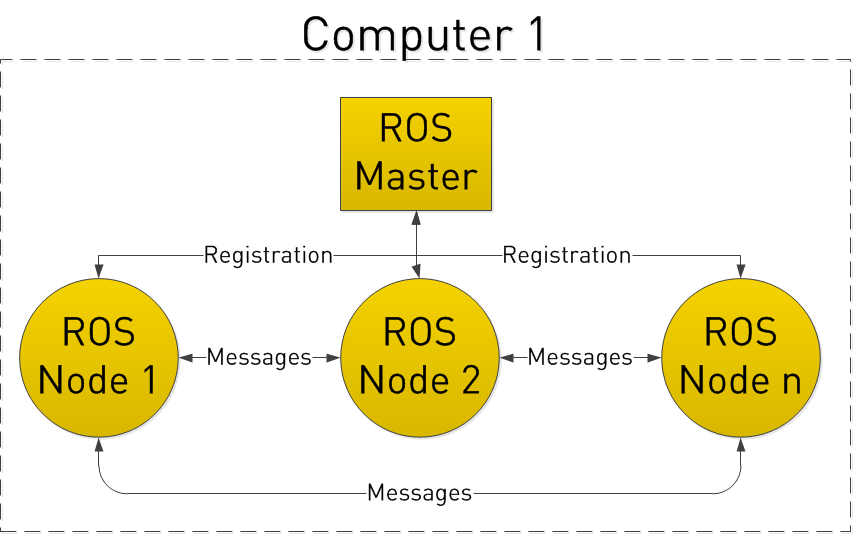
\includegraphics [width=0.8 \textwidth]{imgs/chapter3/rosgraph.png}}
\caption[ROS communication architecture overview]{ROS communication architecture overview \cite{rosbasics}}
\label{fig:rosgraph}
\end{figure}


\subsection{ROS tools}
Now that we described the inner workings of \ac{ROS} we can use its tools to retrieve and analyze information regarding it. We will use the following \ac{ROS} tools:
\subsubsection{rviz}
\textbf{Rviz} is a graphical interface that allows 3D visualization environment that allows the view of the different components of \ac{ROS} like the robots transforms, the map, pointclouds, visualization markers etc...
\subsubsection{rosbag}
\textbf{Rosbag} enables the recording of topics into a file that can be replayed in the future. It is useful to store information and then running it again at the desired time and speed we want.
\subsubsection{rqt_graph}
To understand how the various nodes and topics are interconnected the use of \textbf{rqt_graph} is the best for this case. It can be used to produce an image of all of them and how they communicate between each other
\subsubsection{Command Line tools}
In this section we will highlight some of the command tools in \ac{ROS} that we used in this work.
\subsubsection*{Running ROS Systems}
\begin{itemize}
    \item \textbf{roscore} - this launches all the necessary nodes that the ROS System needs in order to properly setup communication between nodes. It starts the \ac{ROS} Master, Paramater Server and rosout. Using \textbf{roslaunch} will automatically run a roscore if it was not initiated before. 
    \item \textbf{roslaunch} - Used for running multiple ROS nodes as well as setting parameters in the server. This is done by launching ".launch" files that tell which nodes to load, which paramaters to set and what machines it will be used on.
    \item \textbf{rosrun} - Allows you to run a specific exacutable in a predetermined package.
\end{itemize}
\subsubsection*{Debugging and interacting with the \ac{ROS} system}
\begin{itemize}
    \item \textbf{rostopic} - is used for displaying debug information. This may be the messages published by a topic, finding a topic by its type, showing information about a topic, listing all the topics in the \ac{ROS} system. among other things.
   % \item \textbf{rossrv}
    \item \textbf{rosnode} - Can be used to display information regarding publications, subscriptions and connections.
    \item \textbf{rosparam} - Used for getting and setting paramaters in the Paramater Server.
   % \item \textbf{rosmsg}

\end{itemize}
\subsubsection*{Install, build and filesystem tools}
\begin{itemize}
    \item \textbf{rosmake} - Used to build dependencies.
 %   \item \textbf{rosinstall}
    %\item \textbf{roslocate}
\end{itemize}
%%REVER ISTO




%\section{Architecture Overview}\label{ch:requirements}
\section {Navigation Concepts}
There are four main problems associated with robotic autonomous navigation. They are Mapping, Localization, Path Planning and Motion Control \cite{nav} as shown in Fig. \ref{fig:probNav} . 

\begin{figure}[ht!] 
\centerline{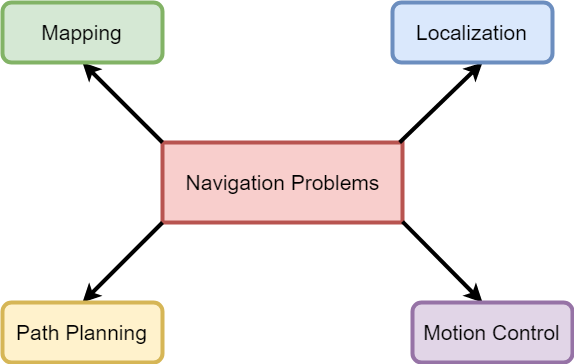
\includegraphics [width=0.8 \textwidth]{imgs/chapter3/navprobs.png}}
\caption{Problems regarding autonomous navigation}
\label{fig:probNav}
\end{figure}
Various algorithms have been developed over the years to combat this problems. 
%%Mapping

In regards to creating a suitable map,  \ac{ROS}  typically uses an improved version of  Rao-Blackwellized particle filters such as the ones described in \cite{grisetti2007improved}. This approach has proven to be an effective way to solve the \ac{SLAM} problem and will be used later on in this work to produce a valid map of our indoor environment.
%%Localization

With the grid map built we now need to estimate the robot's position in said map. 
An easy solution to this problem is relying on the robot's odometry information inferred by the robot's encoders and inertial sensors such as accelerometers and gyroscopes. This is called dead reckoning and is an easy and low cost solution for the localization problem. However since the sensor data is integrated over time, this leads to the accumulation of errors which make this approach not feasible for long navigation tasks. 
To fix this issue various algorithms were developed being the most popular ones based on particle filters. The \ac{AMCL} \cite{amclpaper} algorithm  is the standard choice in this case. It takes into account a group of particles, each one corresponding to a certain robot state (position and orientation in this case). As the robot moves the least probable states are filtered out and  the particles should over time converge on the actual position of the robot.  

Assuming the robot can localize itself on the map with a reasonable error we can start sending navigation goals to the robot. To reach the goal the robot must be able to find a path that optimizes the travel distance while avoiding obstacles. The outputted plan can vary depending on the algorithm used. This type of planning is often refereed as a global path planner that will be discussed further in a section \ref{ppmc} .

After the optimal plan is computed the final step is to determine the best velocity command that will be sent to the base.  The ROS navigation system follows a similar approach to the one used in \cite{gerkey2008planning}. A set of velocities are simulated during a given set of time and the corresponding predicted trajectories are  computed. This subject is often referred to as local path planner methods that will be further detailed in the following section \ref{ppmc}.


\section{Path Planning and Motion Control}\label{ppmc}
 Obstacle avoidance is a major subject in robotics, failure in this systems may result in crashes that have catastrophic consequences such as hardware being badly damaged or being completely nonfunctional. This problem is usually separated into two categories local path planning and global path planning \cite{foxdwa}.
 
 
 Global methods assume the environment is completely known a priori and can therefore compute an optimal safe path  around static obstacles using a variety of different strategies. This models prove to be very reliable for static environments. However this models are usually computational expensive which lead to very slow update times. For fast changing environments such as is in the case for highly populated indoor scenarios they prove to be insufficient. 
 To improve the quality of navigation capabilities, local path planning techniques are added to increase the responsiveness of the robot. This techniques have a much faster update time  since they use a smaller version of the world around them. However this type of approaches have trouble with local minimum cases where the robot gets stuck (for example the U-shape case).
\subsection{Global Methods for Path Planning}
Path planning is crucial for the robot to handle safe trajectory around obstacles. In this work the information regarding this obstacles is based on a grid map built by \ac{SLAM} and new observations retrieved by the robot's sensors.  Planning an optimal safe path can be done using a wide variety of methods like Visibility Graphs, Generalized Voroin Diagram, and \ac{PRM} \cite{globalmethods}. However for in this work we will use the \ac{PRM} method. This method samples its environment and creates a occupancy graph. Then by inserting the initial position and the goal position the path can be computed using dijaktra,A* or Rapidly exploring Random Trees search algorithms . However, the \ac{ROS} navigation packages only use the first two so  we will only focus on this ones.


\subsubsection{Dijkstra algorithm}\label{djk}
Assuming we have an occupancy map we can now start to explain how does a robot compute the shortest path between the starting position and the end goal. Edsgar W. Dijkstra proposed an algorithm that solves this problem for a number of nodes, in our case we have cells on an occupancy grid map. Assuming each cell costs the same then the shortest path can be calculated doing the following algorithm described in Figure \ref{fig:dalg}. 
\begin{figure}[ht!] 
\centerline{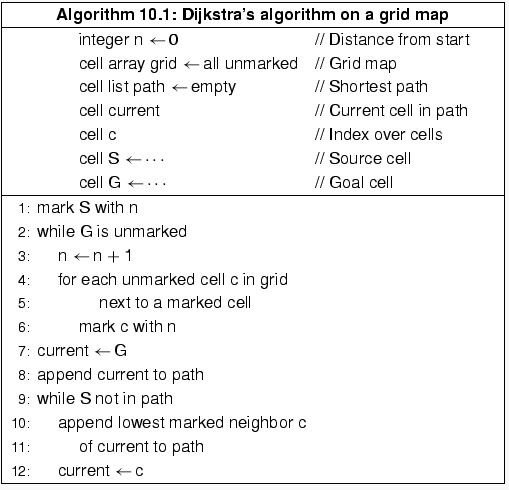
\includegraphics [width=0.7 \textwidth]{imgs/chapter5/Dalg.png}}
\caption[Dijkstra algorithm]{Dijkstra algorithm taken form \cite{Ben-Ari2018}}
\label{fig:dalg}
\end{figure}
Each cell is numbered with the number of steps it needs to get to the starting position. This continues until we reach the goal cell and we get the minimum path to reach it. However if we have a map with cells that have variable cost in the algorithm above we do not iterate $n$ with plus one, but with the cell cost. This makes it so for this case that  shortest path geometrically may not be the shortest path when the costs are taken into account.

\subsubsection{A* algorithm}\label{A*}
In the previous case we search for cells in all directions, however there is a more efficient way of doing it by adding more information. The A* algorithm besides the cost from the steps to the start position$g(x,y)$,it takes into account an extra \textit{heuristic function} $h(x, y)$ to that gives a preferred direction for the search. Not only does it take into account the cell cost but another value that corresponds to a given direction to be doing in  the search. The function can be shown as:
\begin{equation}
    f(x,y)=g(x,y) + h(x,y)
\end{equation}
\subsection{Local Methods for Motion Control }
In contrast to global path planning in where a large portion of the environment is generally assumed to be true, local methods take in to account a partial world view for motion planning capabilities. In other words, local path planning determines the motion of the robot taking into account the global plan provided by the global methods described earlier.
The most popular of this type of methods are \cite{inbookdwa}:
%cite this
\begin{description}
    \item [\ac{DWA}] -  \cite{foxdwa} Takes into account a substet of admissible velocities taking into account robot's dynamic constraints and simulates them for a given time frame outputting various trajectories. Then using this trajectories derives the best trajectory given a certain cost function.  
    \item [Trajectory Rollout]  \cite{gerkey2008planning} - Similar to the \ac{DWA} planner except the sampling method for the control space is different.
    \item [Elastic Band] - \cite{siegwart2011introduction} In this case bubbles are formed that are defined as the maximum local subset of free space around a given robot configuration that can be travelled without collision.
    Given this bubbles a set of "elastic bands" can be connected to form a collision free trajectory from the initial position to the goal without collision. When it comes to avoid an obstacle that obstructs the global plan, this technique tends to deviate from it  minimizing the bubble band tension.
    \item [Timed elastic band] - \cite{rosmann2013efficient} This planner is an extension of the 'elastic band' that takes into account time intervals in between the robot's configurations. By doing this and utilizing a  multiple objective optimization function that takes into account the robot's accelaration and velocity limits with penalties and computes the best trajectory taking into account execution time, shortest path and clearance of obstacles it creates a suitable local planner that is suitable for avoiding dynamic obstacles.
    
    \item [Tentacles Clothoid] -  \cite{ffalia2015local} This is an empirical approach to the local path planning problem. It generates various "tentacles" and take the form of clothoids. It then chooses the best one taking into account the best obstacle clearance, curvature and distance to the global path planner. 
    
    \item [\ac{VFH}+] \cite{siegwart2011introduction} - For this approach first an histogram of the ammount of obstacles in a certain direction is first created.Then using a cost function that takes into account the alignment of the robot towards the goal, the difference between the new direction and the current wheel orientation and the difference between the previously selected direction and the new direction is computed. The best trajectory is then chosen taking into account this information.
    
\end{description}
For our case study we will only explore the first two in detail since that they are already implemented in ROS.
\subsubsection{DWA planner}\label{dwa}
The \ac{DWA} planner is the most standard approach when it comes to local path planning in \ac{ROS}. It outputs  rotational and translational velocity by generating multiple trajectories for different types of velocity sample search space and choosing the best one. The algorithm goes as follows \cite{inbookdwa}:
\begin{itemize}
    \item Start with a set of velocities pairs $\{R_{vR_x},R_{ \omega_z} \}$ that are obtainable by the robot.
    \item Genarate in the form of arcs the projected trajectories obtained using the previous velocity sample space.
    \item Dismiss velocities that result in the robot colliding with an object in a given time frame. With this we are left of a subset of admissible velocities $V_a=R_{vR_a},R_{ \omega_a}$ in which:
    \begin{equation}
         V_a=R_{vR_a},R_{ \omega_a} \iff \begin{cases}
    R_{vR_x} & 	\leq \sqrt{2*dist(R_{vR_x},R_{ \omega_z})*R_{\dot{v}_{xb}}}.\\
    R_{ \omega_z}  &  	\leq \sqrt{2*dist(R_{vR_x},R_{ \omega_z})*R_{\dot{\omega}_{zb}}}.
  \end{cases}
    \end{equation}
    Where $R_{\dot{v}_{xb}}$ and $R_{\dot{\omega}_{zb}}$ are the braking accelerations of the robot and $dist$ the distance to the closest obstacle on the trajectory.
    
    
    \item Dismiss velocities that don't respect the robot's acceleration limits in a given simulated time frame. With this we are left with a subset of velocities called dynamic window $V_d=R_{vR_d},R_{ \omega_d}$  in which:
    \begin{equation}
         V_d=R_{vR_d},R_{ \omega_d} \iff \begin{cases}
    R_{vR_x} & 	\in [R_{v_a}-R_{\dot{vR}_{x}}*t,R_{v_a} + R_{\dot{vR}_{x}}*t].\\
    R_{\omega_z} & 	\in [R_{ \omega_a}-R_{\dot{\omega}_{z}}*t,R_{\omega_a}+R_{\dot{\omega}_{z}}*t].\\
  \end{cases}
    \end{equation}
    \item Finally we choose  the most optimal trajectory and in consequence velocity pair taking into account a given objective cost function.
    \end{itemize}
\subsubsection{Trajectory Rollout} \label{tr}
The Trajectory Rollout planner follows the same logic as above but in this case the sampling method for the control space is different. In this a set permissible velocities
in each simulation is calculated including acceleration limits for the entire simulation time\cite{inbookdwa}.Instead of searching the space of feasible trajectories, we search the space of feasible controls. In Trajectory Rollout set of permissible velocities in each simulation is calculated including acceleration limits for the entire simulation
time, while in Dynamic Window Approach it is limited to one simulation step.
\section {ROS Navigation stack}
The ROS navigation stack is a set of software packages that properly combined can get a robot to navigate autonomously.
Figure \ref{fig:plans} shows an example of \textbf{turtlebot2} using the navigation stack to drive autonomously.
\begin{figure}[!htb]
    \centering
    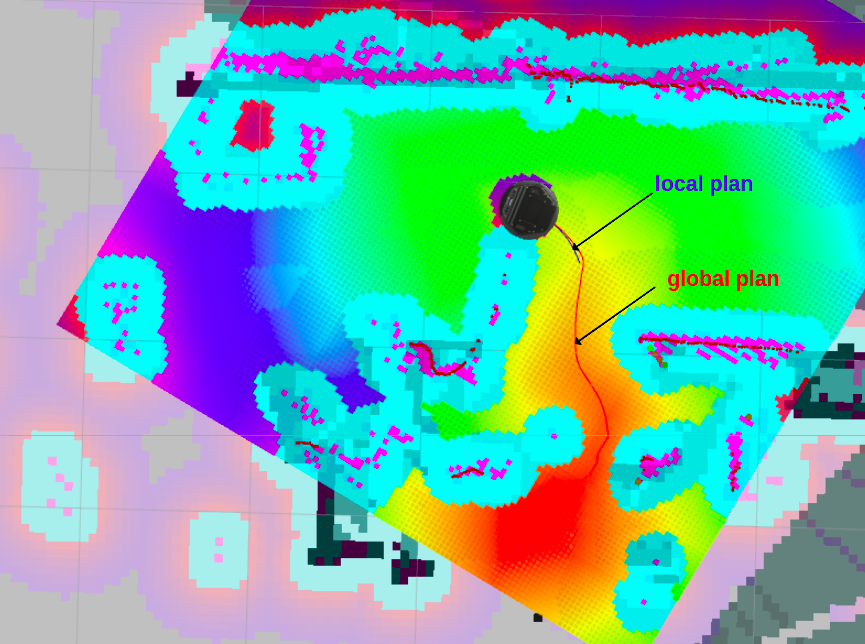
\includegraphics[width=\linewidth]{imgs/chapter3/nav.png}
    \caption[Rviz view of the ROS Navigation Stack]{Rviz displaying the ros navigation stack components while \textbf{turtlebot2} is navigating.}
    \label{fig:plans}
\end{figure}

\subsection{Requirements}
 Before running the \ac{ROS} navigation stack we first need to properly setup the robot that meet its requirements.
\subsubsection{Transform Configuration}
The Navigation stack requires that the relationships between the different frames must be published in \textbf{tf} or \textbf{tf\_static} topic. This makes it so the robot perceives what is around him correctly.
Figure \ref{fig:tf} shows all the frames and their transforms with each other for \textbf{turtlebot2}. However the main transforms that need to be correct are between the sensors and the base link frame.
\begin{figure}[!htb]
    \centering
    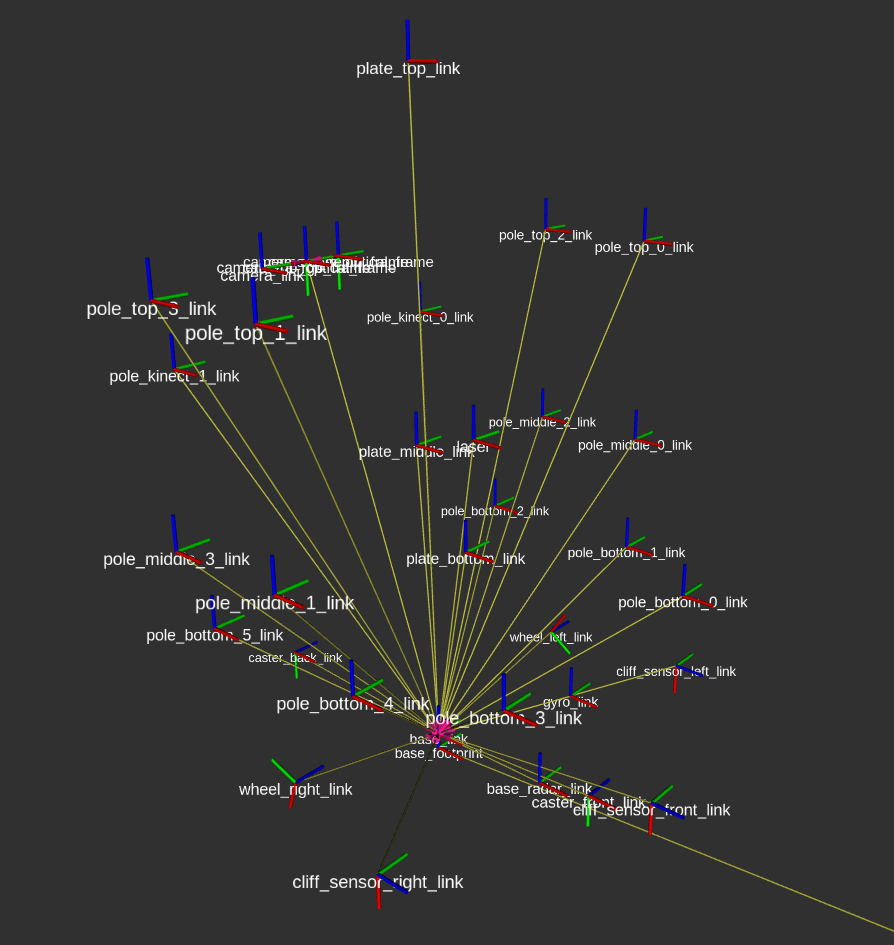
\includegraphics[scale=0.4]{imgs/chapter3/tf.png}
    \caption{Example of the transform relationships}
    \label{fig:tf}
\end{figure}

\subsubsection{Sensor sources}
To avoid obstacles we need some type of sensors that can detect them. Before running the stack we need to make sure they are publishing this information.
In our case we will use both the \textbf{\ac{FMCW}} \textbf{\ac{radar}} (PointCloud2) and the \textbf{\ac{LiDAR}} (LaserScan) as our observation sources.
Figure \ref{fig:sensors} shows an example of the published data from both in rviz.
\begin{figure}[!htb]
    \centering
    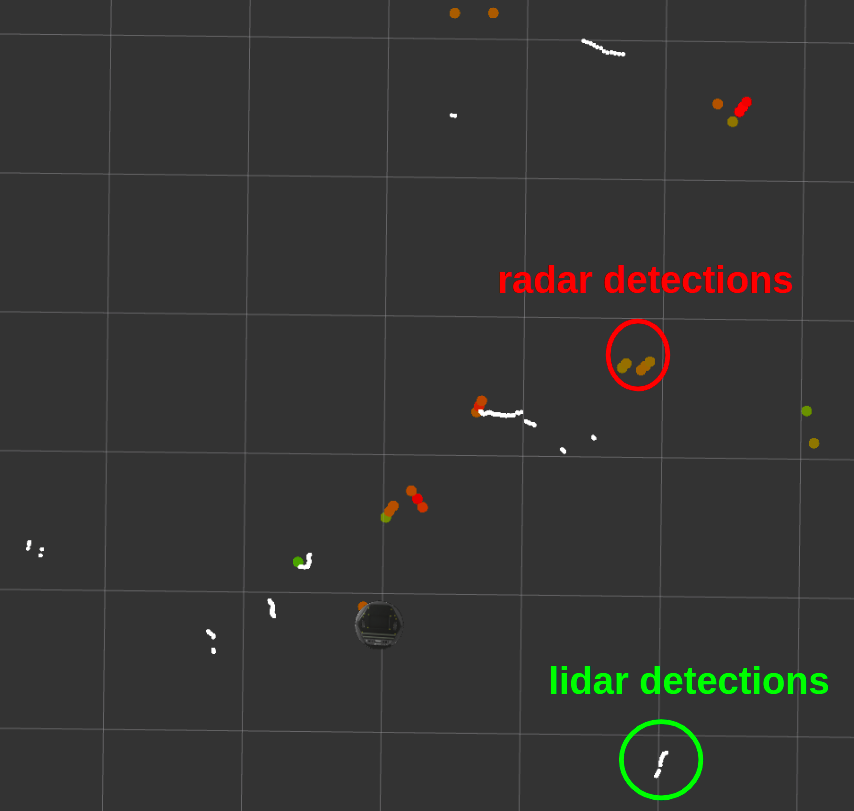
\includegraphics[scale=0.5]{imgs/chapter3/sensors2.png}
    \caption{Obstacle detections by both radar and lidar}
    \label{fig:sensors}
\end{figure}
\subsubsection{Odometry}
We need to localize the robot in some way to correctly navigate. Therefore we require a topic that publishes odometry information.
\subsubsection{Base Controller}
This node will subscribe to the velocity message outputted by the navigation stack and convert them into the appropriate motor commands to send to the mobile base that will actually make the robot move.
%%GARBAGE
\subsubsection{Mapping}
This part is not mandatory but it helps to have a some sort of map being published to use as a global reference for the robot. It is used by \texttt{amcl} to correctly localize the robot and to mark previously detected lethal obstacles when the map was built. Fig. \ref{fig:map} shows an example of a map that might be used by the ROS navigation stack.
\begin{figure}[!htb]
    \centering
    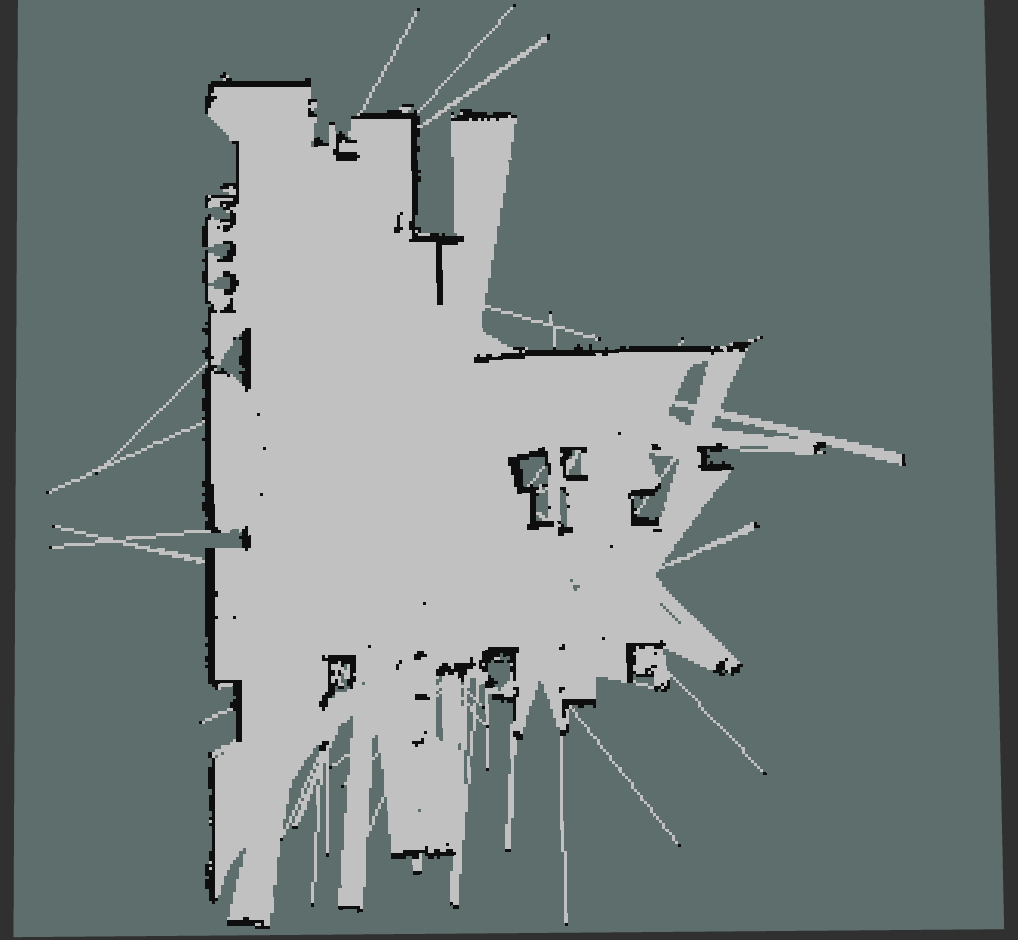
\includegraphics[scale=0.4]{imgs/chapter3/map2.png}
    \caption{Example of a map created in the IRIS laboratory}
    \label{fig:map}
\end{figure}
If the setup is done correctly we can now run the navigation stack.
\subsection{Navigation Stack components}
%%STUFF
Now that we have all the things we need for navigation we need an entity that actually processes all this information in an intelligent way to determine the best velocity command for the robot. This is done by the \texttt{move\_base } node and its peripherals.
Figure \ref{fig:navstack} shows an overview of the different components of the navigation stack \cite{movebase}.
\begin{figure}[!htb]
    \centering
    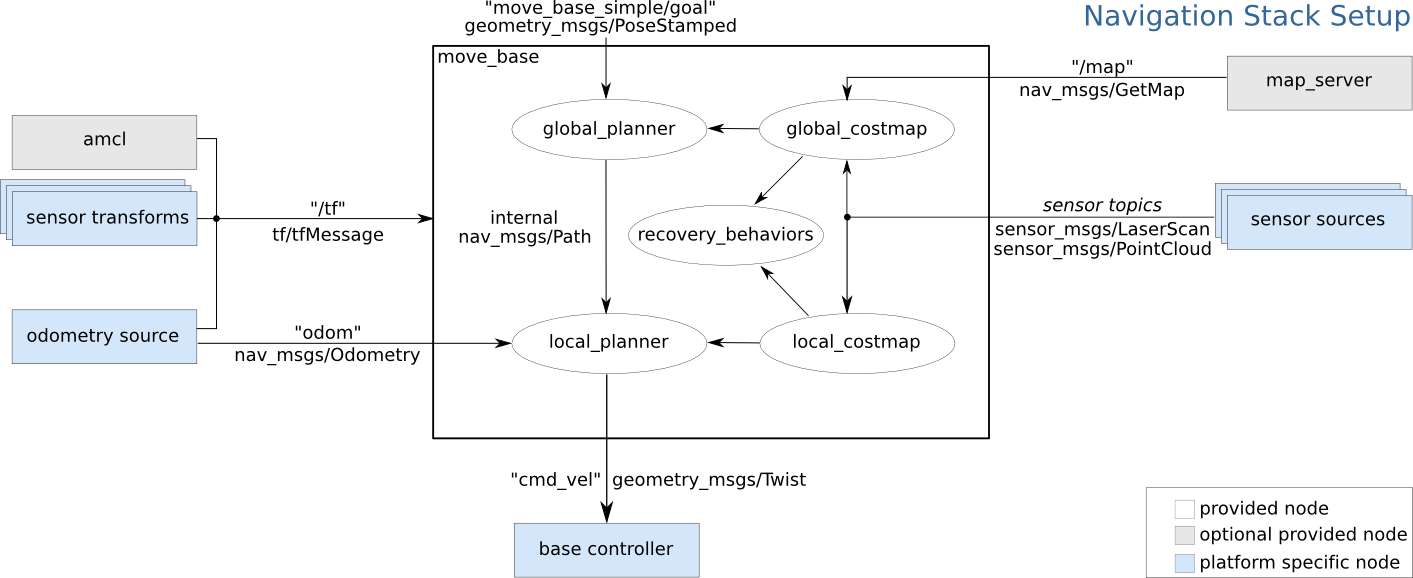
\includegraphics[width=\linewidth]{imgs/chapter3/navstack.png}
    \caption[Navigation stack block diagram]{Navigation stack block diagram taken from \cite{movebase}}
    \label{fig:navstack}
\end{figure}
\subsubsection{Move Base}

The move base node base links together a global and local planner as well as a local and global costmap to achieve the end goal provided by an action server. It also loads a set of determined recovery behaviors if the planners fail to produce a valid path. 

The global and local planners are plugins specified by the user. This choice will affect the behavior of the robot depending on the planners architecture and parameters. In this work it will be used \textbf{navfn} as our global planner and \textbf{TrajectoryPlannerROS} as our local planner.

\subsubsection{Global Planner}
 
The job of this component is to produce the best trajectory for a robot to take with limited amount of information given by the global costmap.
This plan can be updated when the robot gets stuck or by a user specific frequency the latter is usually preferred. The algorithms used to get this path are usually \textbf{djakarta} or \textbf{A*} that are described in the previous sections \ref{djk} and \ref{A*}.

\subsubsection{Local Planner}
The local planner takes into account the trajectory given by the global planner and tries to compute velocity commands that follow it. However the path given may be to close to an obstacle detected and in order to avoid it we must deviate from the plan given to avoid collision. The function of the local planner is to avoid dynamic obstacles that appear while still trying to follow the global plan and goal. This type of local planner is usually \textbf{TrajectoryPlannerROS} or \textbf{DWAPlanner} that follow the explanation in the previous sections \ref{dwa} and \ref{tr} and uses the local costmap to do so. Bellow we define how \textbf{TrajectoryPlannerROS} generates the best trajectory using a determined cost function.

\subsubsection*{Getting the Best Trajectory}
The algorithm to get the best trajectory goes as follows:
\begin{enumerate}
    \item Discreetly sample the velocity space ($d_{vx}$ and $d_{vtheta}$)
    \begin{align*}
        & d_{vx}=(\texttt{max\_vel\_x}-\texttt{min\_vel\_x})/\texttt{vx\_samples}\\
         & d_{vtheta}=(\texttt{max\_vel\_theta}-\texttt{min\_vel\_theta})/\texttt{vtheta\_samples}
    \end{align*}
    \item For each sampled velocity predict its trajectory in a given time frame (\texttt{sim\_time}).
    \item Evaluate the cost of each trajectory  by using the value cost function
    \item Pick the one with lowest cost and publish the associated velocity.
    \item Repeat for a given rate (\texttt{controller\_frequency})
\end{enumerate}
\subsubsection*{Cost Function}
As described earlier the cost function used to evaluate a trajectory is given by:
\begin{align*}
        \textbf{cost} = &
   \texttt{pdist\_scale} * \textbf{path\_dist}
   + \texttt{gdist\_scale} * \textbf{goal\_dist}\\
   &+\texttt{occdist\_scale} * \textbf{maxobscost} 
\end{align*}

Where \textbf{path\_dist} is the distance from the endpoint of the trajectory to the global path in map cells, \textbf{goal\_dist} is the distance from the endpoint of the trajectory to the local goal in map cells, and \textbf{maxobscost} is equal to the \textbf{maximum obstacle cost} (given by the local costmap) of all the points along the trajectory.
Fig. \ref{fig:costcloud} displays an example of this values when the robot is navigating.
\begin{figure}[!htb]
    \centering
    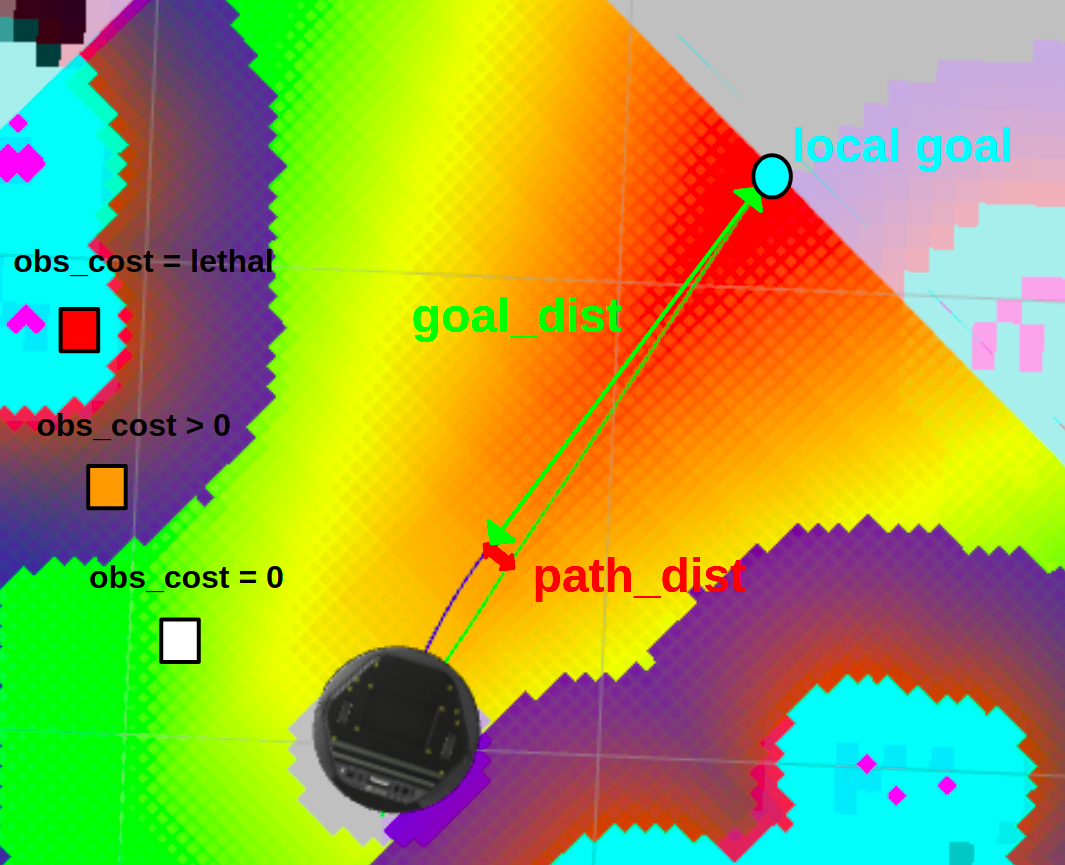
\includegraphics[width=0.8\linewidth]{imgs/chapter3/costcloud.png}
    \caption[Cost cloud published in rviz]{Cost cloud published in rviz. Red cells correspond to low cost and green cells correspond to a high cost}
    \label{fig:costcloud}
\end{figure}
\subsubsection{Local and Global Costmap}
The global and local costmap share the same class, the  \texttt{Costmap2DROS}. This class consists of a layered costmap that takes into account various layers defined by the user.

\subsubsection*{Available Layers}
\begin{itemize}
    \item \textbf{Obstacle Layer} - Marks objects retrieved from our sensor sources with lethal value. It also raytraces observations to clear out space.
    %Does more stuff
    \item \textbf{Inflation Layer} - Inflates the detected obstacles taking into account the robot radius and inflation radius. The closer the cells are from a lethal obstacle the more value they will have.
    %%....(needs explanation)
    \item \textbf{Static Layer} - Retrieves static information from the \textbf{/map} topic and marks them has lethal objects (Typically only used in global costmap).
\end{itemize}

Figure \ref{fig:layers1} shows how the combined layers produce the master costmap that will be used by the planners \cite{lu2014layered}.

\begin{figure}[!htb]
    \centering
    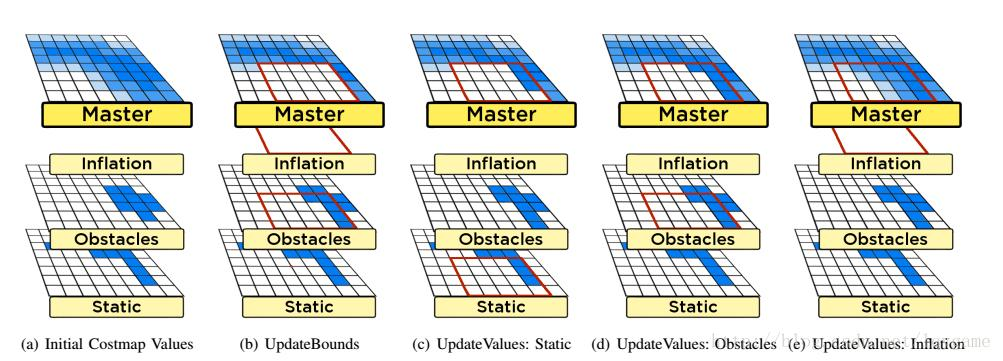
\includegraphics[width=\linewidth]{imgs/chapter3/layers1.png}
    \caption[Various costmap layers that together form the master costmap]{Various costmap layers that together form the master costmap that will be used in the global or local planner from \cite{lu2014layered}}
    \label{fig:layers1}
\end{figure}
\section{Summary}
In this chapter we described the inner workings of the ROS framework and what tools can be used in order to develop a certain application. We also discussed what types of problems exist in regards to autonomous navigation. Finally we showed how the ROS navigation stack tackles this issues in order to construct a safe navigation module for our robot.



\cleardoublepage
\chapter{Robotic Navigation Platform }

In this section we will describe the principal components in terms of hardware and software and how they are interconnected to create a suitable robotic platform that will later be used for comparing the performance of \ac{LiDAR} and \ac{FMCW} \ac{radar} as obstacle avoidance sensors.


\section{Hardware}
The basic hardware for this work will be a  modified version of the  turtlebot2 platform,
The out of the box kobuki platform was modified in order to include a processing unit, a 2D scanning \ac{LiDAR} and a \ac{FMCW} radar as proximity sensors. The modified version is displayed in Fig.\ref{fig::turlebot2M}. 

\begin{figure}[ht!] 
\centerline{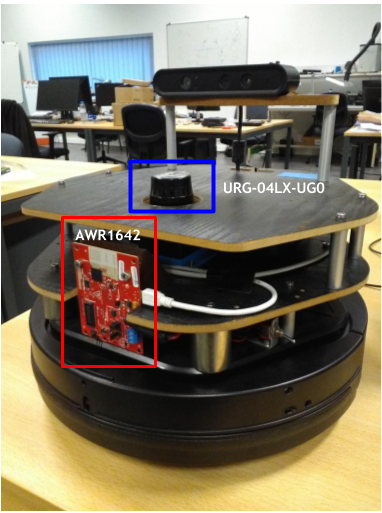
\includegraphics [width=0.4 \textwidth]{imgs/chapter4/turtlebot2.PNG}}
\caption{Modified Turtlebot2 used in this work}
\label{fig::turlebot2M}
\end{figure}

\subsection{Turtlebot2}
TurtleBot 2 (Fig. \ref{fig:t2}) is one of the  most popular low cost personal robots around. It is completely run by open source software which makes it exceptional for research and educational purposes. The robot has been developed by the Korean company Yujin Robotics in collaboration with Willow Garage, its differential kinematics mobile platform can be used for multiple applications, due to the huge number of available ROS packages. It comes with a kobuki base a processing unit Intel NUC, the 2-D \ac{LiDAR} Hokuyo URG-04LX-UG01 Scanning Laser Rangefinder and finally a Kinect for XBOX 360.

\begin{figure}[ht!] 
\centerline{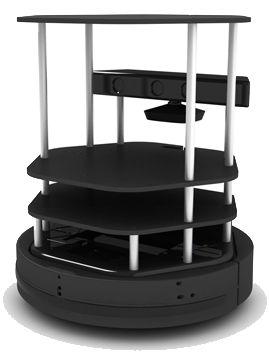
\includegraphics [width=0.3 \textwidth]{imgs/chapter4/turtlebot2.png}}
\caption{Turtlebot 2 platform}
\label{fig:t2}
\end{figure}

\subsubsection*{Technical Specifications}
When it comes to technical specifications the robots dimension is 354 x 354 x 420 mm as shown in Fig. \ref{fig::t2specs}, its weight is 6.3 Kg with a max payload of 5 Kg which means it is able to attach lots of devices with relatively heavy if needed. The maximum translational  speed of it is 0.7 m/s and the maximum rotational speed is 180º/s . It as a gyroscope with 1 axis(110º/s), odometer at 52 ticks/encoder and  bumpers on left right and center among other components. 

\begin{figure}[ht!] 
\centerline{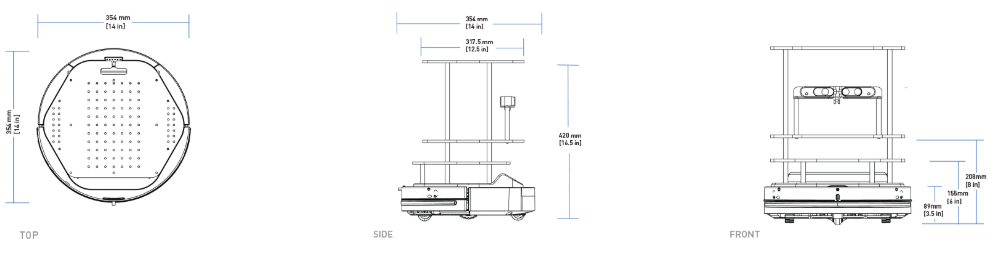
\includegraphics [width=1.0 \textwidth]{imgs/chapter4/tspecs.png}}
\caption{Turtlebot 2 dimension specifications}
\label{fig::t2specs}
\end{figure}


\subsection{FMCW radar}
The radar board chosen for this work is the mmwave \ac{TI} AWR1642BOOST (Fig.\ref{fig:awr}). This is a recently distributed \ac{FMCW} radar dedicated for short range applications. It is an easy-to-use evaluation board for the AWR1642 automotive radar sensor which is connected to the micro-controller unit (MCU) LaunchPad. To develop software it has  on-chip C67x DSP core and low-power ARM Cortex-R4F controllers which include onboard emulation for programming and debugging.
It requires a 5V > 2.5 A supply brick with a 2.1-mm barrel jack to run.
The device supports a wide RF bandwidth of 77-81 GHz that permits good range, velocity  and angle resolution. This last parameters depend on the configuration fed to the device.

\begin{figure}[ht!] 
\centerline{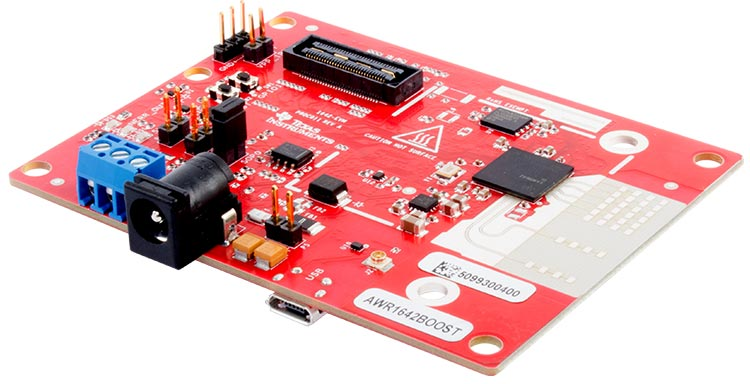
\includegraphics [width=0.5 \textwidth]{imgs/chapter4/awr1642.jpg}}
\caption{Texas Instruments AWR1642BOOST evaluation board}
\label{fig:awr}
\end{figure}


The radiation pattern of the antenna in the horizontal plane (H-plane Phi = 0 degrees) and elevation plane (E-plane Phi= 90 degrees) is shown by Figure \ref{fig:el}.
\begin{figure}[ht!] 
\centerline{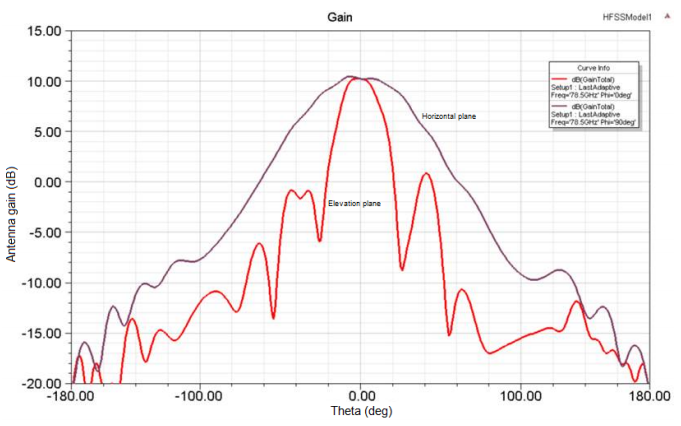
\includegraphics [width=0.9 \textwidth]{imgs/chapter4/elevation.png}}
\caption{Radiation pattern of the antenna from \cite{el}}
\label{fig:el}
\end{figure}

\subsection{LiDAR}
Besides the \ac{FMCW} \ac{radar} the Hokuyo URG-04LX-UG01 Scanning Laser Rangefinder (Fig. \ref{fig:lidar}) is also attached to the platform.

\begin{figure}[ht!] 
\centerline{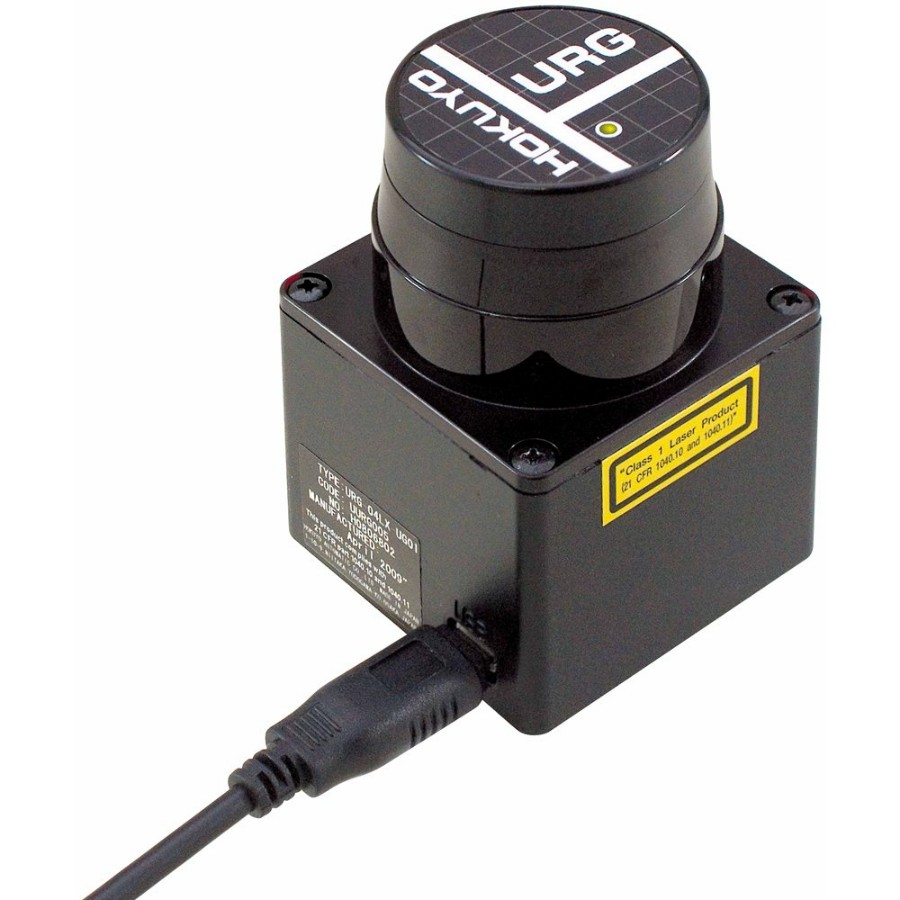
\includegraphics [width=0.5 \textwidth]{imgs/chapter4/lidar.jpg}}
\caption{Hokuyo URG-04LX-UG01 Scanning Laser Rangefinder}
\label{fig:lidar}
\end{figure}

This sensor is an inexpensive 2D-\ac{LiDAR} that is based on phase difference measurement. It retrieves information of the surrounding environment by scanning an area of 240º with 0.36º angular resolution. The maximum range of it is about 4 meters and its range resolution is 1mm. Its scan update time is 100ms/scan and its weight is 360 g.  As for the power supply it only needs a 5V DC provided by the USB connection as shown in figure \ref{fig:lidarS}.



\begin{figure}[ht!] 
\centerline{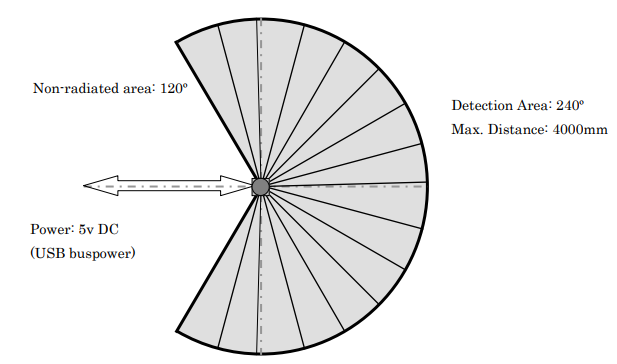
\includegraphics [width=0.6 \textwidth]{imgs/chapter4/lidarS.png}}
\caption{Hokuyo URG-04LX-UG01 specifications diagram}
\label{fig:lidarS}
\end{figure}




\section{Software}
In order to produce a suitable platform for navigation we need to interconnect various software modules in \ac{ROS}. First a map of the environment is created by the 2-D \ac{LiDAR} using the package \texttt{gmapping}. After that is done we launch the \texttt{amcl} node that will update the localization of the robot taking into account odometry information and the surrounding environment. After that is done we have a robot that is reasonably well localized. Now all we need is to feed some sensor sources to the navigation module that will act as obstacle detectors.

To do that, first the interface between the radar board TLV data and the ROS point cloud message format is done using the provided radar driver from Texas Instruments.  Then a filter by intensity operation is added to remove false positive detections (this will be explained later). The filtered radar data as well as the \ac{LiDAR} data are fed to the Navigation module as sensor sources.


Figure \ref{fig::softsetup} shows the block diagram describing  the different modules used to have a proper autonomous navigation platform.
\begin{figure}[h] 
\centerline{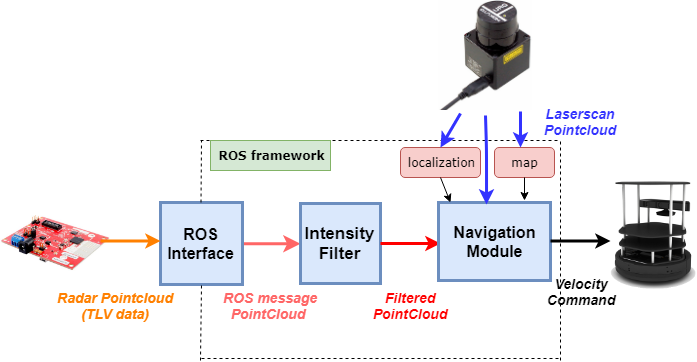
\includegraphics [width=0.9 \textwidth]{imgs/chapter4/bd.png}}
\caption{Block diagram of the software modules used in this work}
\label{fig::softsetup}
\end{figure}

\subsection{ROS radar driver}
Texas Instruments provides a ros package that interfaces radar data to the ROS message format \cite{tisetup}. The incoming radar TLV data from the mmWave EVM is decoded in order to create a  \textbf{PointCloud2} type ROS message.
This point cloud follows the detected objects frame described in the mmWave demo data structure \cite{mmdata} represented in Fig. \ref{fig:demodata}.
\begin{figure}[!htb]
    \centering
    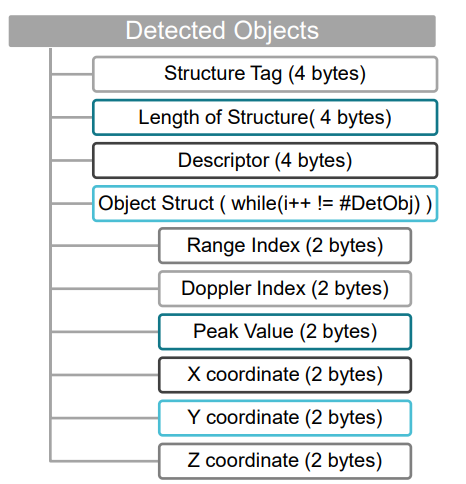
\includegraphics[scale=0.8]{imgs/chapter4/demodata.png}
    \caption[Part of the mmwave demo packet]{Part of the mmwave demo packet containing object detection information. This fields will be used to construct the ROS PointCloud2 \cite{mmdata}.}
    \label{fig:demodata}
\end{figure}
Each point has 6 fields:
\begin{itemize}
\item \textbf{x (m)} - position x of the detected  object in the frame of the radar.
\item \textbf{y (m)} - position y.
\item \textbf{z (m)} - position z (for 2D devices this is equal to zero).
\item \textbf{range (m)} - range of the object relative to the radar frame.
\item \textbf{doppler (m/s)} - radial velocity of the object relative to the radar frame.
\item \textbf{intensity} - relative power of the received signal corresponding to that object.
\end{itemize}
\subsubsection{Chirp profile configuration file}
The characteristics of this point cloud such as publishing rate, range resolution, maximum range, velocity resolution, maximum velocity depends on the chirp profile configuration file loaded in the EVM. This file is located in the \textbf{"cfg"} folder of the ti mmwave package and can be replaced in order to accommodate a given application.

The easiest way to create a chirp configuration file is the mmWave Demo Visualizer. With it you can auto generate a configuration file given a set of specifications.
Another way of doing this is manually. This however requires the understanding of the radar operating principle and the configuration commands.



\subsection{Point Cloud Library}
%Describe PCL
Since we are dealing with point clouds coming from the \ac{FMCW} \ac{radar} and the 2-D\ac{LiDAR} than we need some type of ways to handle and manipulate them. For that the open source libraries called \ac{PCL} is the more indicated place to process and manipulate this type of information. A pointcloud is a collection of multi-dimensional points and is commonly used to represent three-dimensional data \cite{pcl}. This points are often just designed to locate points in x,y,z but more dimensions can be added as is for the FMCW radar which has 6 dimensions. \ac{PCL} provides open source state of the art library modules that enables  filtering, feature estimation, surface reconstruction, registration, model fitting and segmentation. In our case we will mainly use its passthrough filters and for constructing visualization markers that show the \ac{radar} information in a more intuitive way.

\subsection{Visualization of the radar point cloud}
Plotting the points in the XYZ space is not enough to fully visualize the radar data sent since each point also gives velocity and intensity information.

We can visualize it by using markers such as arrows or text in rviz.
Figure \ref{fig:doppler_marker} displays the radial velocity of each point with an arrow. The size of the arrow indicates how fast the object is going. Figure \ref{fig:intensity_marker} shows the intensity values of each object in text. This type of visualization will be useful when we try to filter the cloud.


\begin{figure}[!htb]
    \centering
    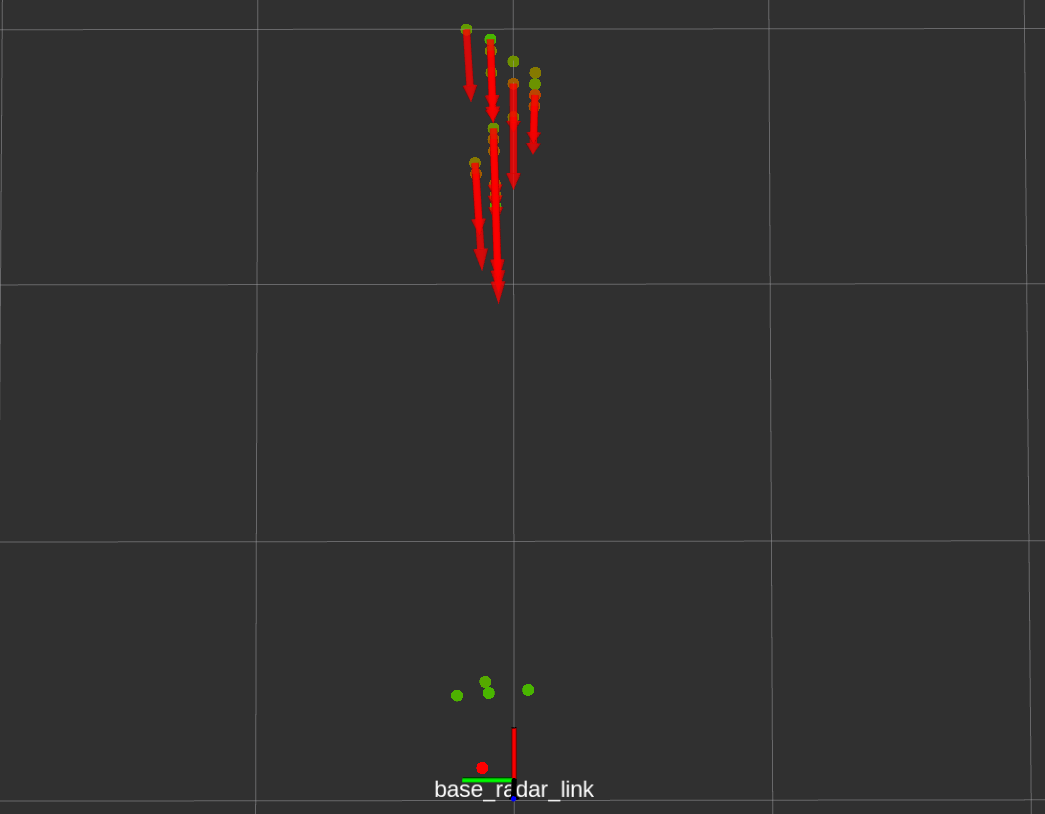
\includegraphics[scale=0.25]{imgs/chapter4/dopplermarker.png}
    \caption{Arrow markers displaying the points radial velocity}
    \label{fig:doppler_marker}
\end{figure}

\begin{figure}[!htb]
    \centering
    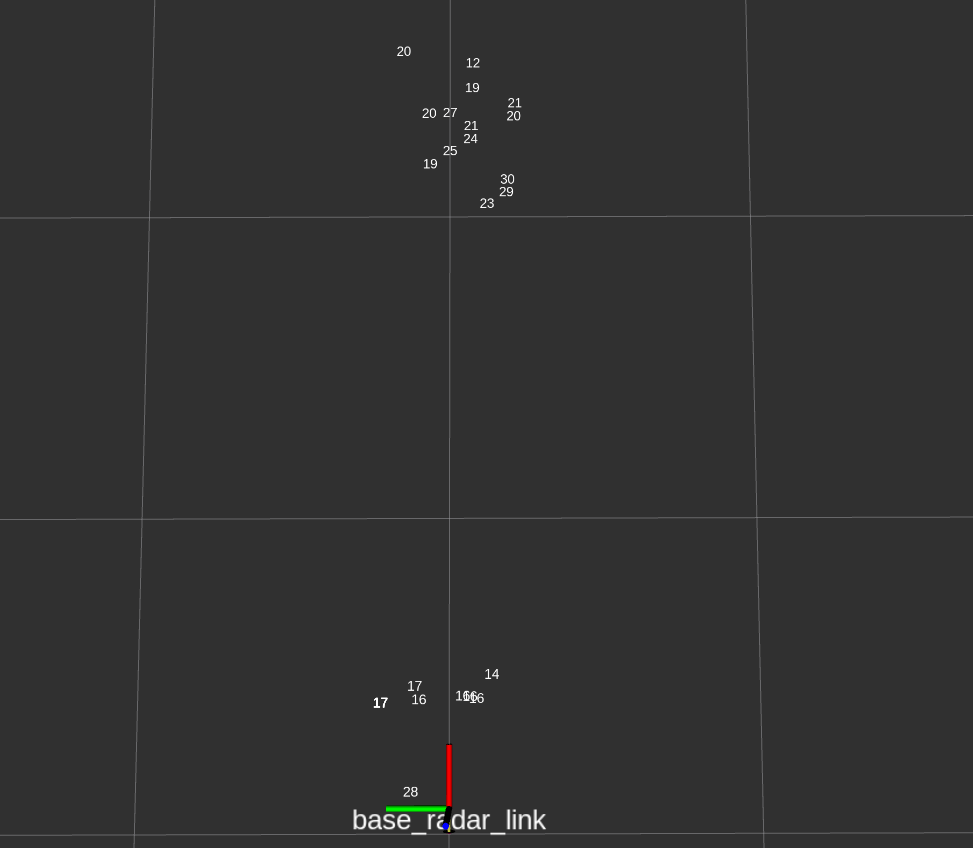
\includegraphics[scale=0.25]{imgs/chapter4/intensitymarker.png}
    \caption{Text markers displaying the points intensity values}
    \label{fig:intensity_marker}
\end{figure}




\subsection{Radar Data Processing}
Now that we have the radar constantly giving us a point cloud we can further process to retrieve the information we want. 
In our case we will make use of \textbf{passthrough filters} to remove unwanted points. This operations will be done by using the \textbf{Point Cloud Library}.
%and \textbf{euclidean clustering} to identify groups of points that belong to the same object.
\subsubsection{Passthrough Filters}
In the point cloud there may be some points that have undesirable characteristics, such as points with low intensity  that lead to false detections or outside of the radar operating range. To remove this points we use \textbf{passthrough filters} that specify the range of values a given field can have in order for a point to be kept in the point cloud. 

For example, if we are only interested in obstacles that are moving between 0.5 m/s and 1.0 m/s (radial velocity), this can be done by using a passthrough filter on the doppler channel.
Figure \ref{fig:filters} shows an example where we delete false detections close to the radar by filtering the point cloud by intensity. In this work we will use an intensity filter of 16, which means alll target points that have an intensity bellow that will be filtered out due to having low \ac{SNR}


\begin{figure}[ht!] 
    \begin{minipage}[b]{.49\linewidth}
        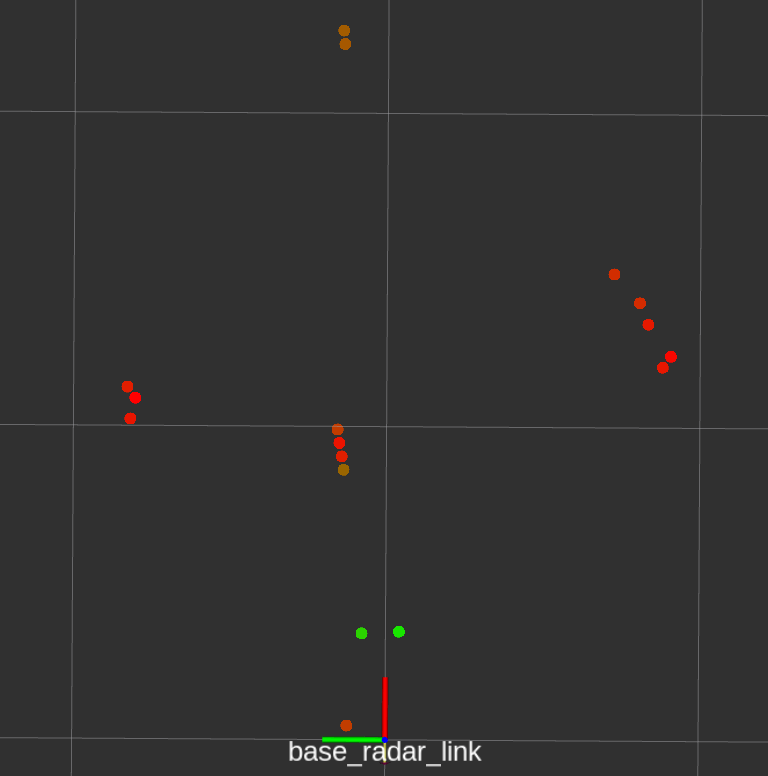
\includegraphics[height=5cm,width=\linewidth]{imgs/chapter4/notfilt.png}
        \subcaption{Non filtered pointcloud}
        \label{fig:fft}
    \end{minipage}
    \begin{minipage}[b]{.49\linewidth}
        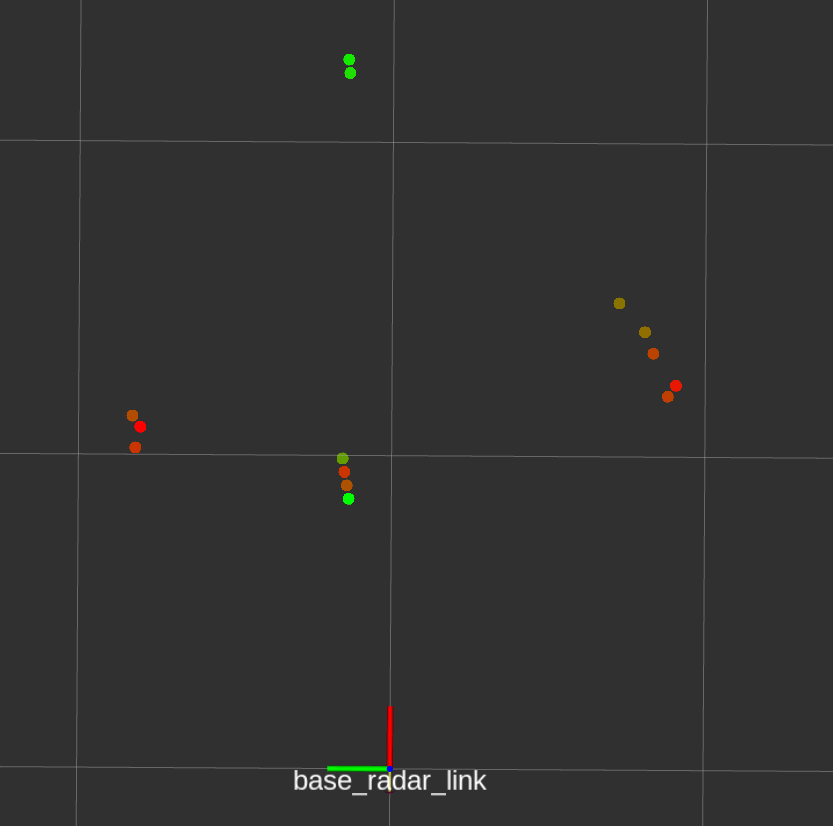
\includegraphics[height=5cm,width=\linewidth]{imgs/chapter4/filt.png}
        \subcaption{Filtered pointcloud by intensity}
        \label{fig:fft2}
    \end{minipage}
    \caption{Example of filtering the pointcloud}
    \label{fig:filters}
\end{figure}


\section{Summary}
In this chapter we over viewed the technical specifications of each hardware component in the navigation platform. We also describe what software and how its interconnected  to properly setting up the turtlebot robot for indoor navigation using the \ac{FMCW} \ac{radar}.


%The software used in this project is divided in a few stages. First the interface between the radar board TLV data and the ROS point cloud message format is done using the provided radar driver from Texas Instruments.  Then a filter by intensity operation is added to remove false detections (this will be explained later). The filtered radar data as well as the \ac{LiDAR} data are fed to the ROS Navigation Stack as sensor sources. In terms of mapping a f
\cleardoublepage
\chapter{Experimentation and Results}


Over the course of this work it was concluded that the radar data was not appropriate for Map Building or for localization using \ac{AMCL}. However it was noted that the radar was quicker   at detecting different types of obstacles. 
With the configuration described in the previous section we can now start to experiment with the robotic platform to do certain navigation tasks. In this part we propose various experiments that try to evaluate the  performance of the \ac{FMCW} \ac{radar} as an alternative or support to the \ac{LiDAR} as an obstacle detector for indoor navigation.




\section {Static Obstacles in controlled environment}
In this work the \ac{FMCW} radar has shown to have better performance at detecting certain indoor objects than the 2D \ac{LiDAR}. This means that there might be situations where using it for obstacle avoidance produce better results for indoor navigation tasks. \\

To demonstrate this a test was devised in a controlled environment that compares the performance of each sensor for different types of obstacles, in this case two types of chairs, a garbage bin, a low height box, a transparent acrylic tube and finally a robot (in this case another tutlebot2).  
%We also try to use the fusion of both sensors that in theory should produce the best results. 
To ensure the experiment is done in a controlled way the scenario shown in Figure \ref{fig:cenario} was constructed. 
\begin{figure}[ht!] 
    \begin{minipage}[t]{.49\linewidth}
        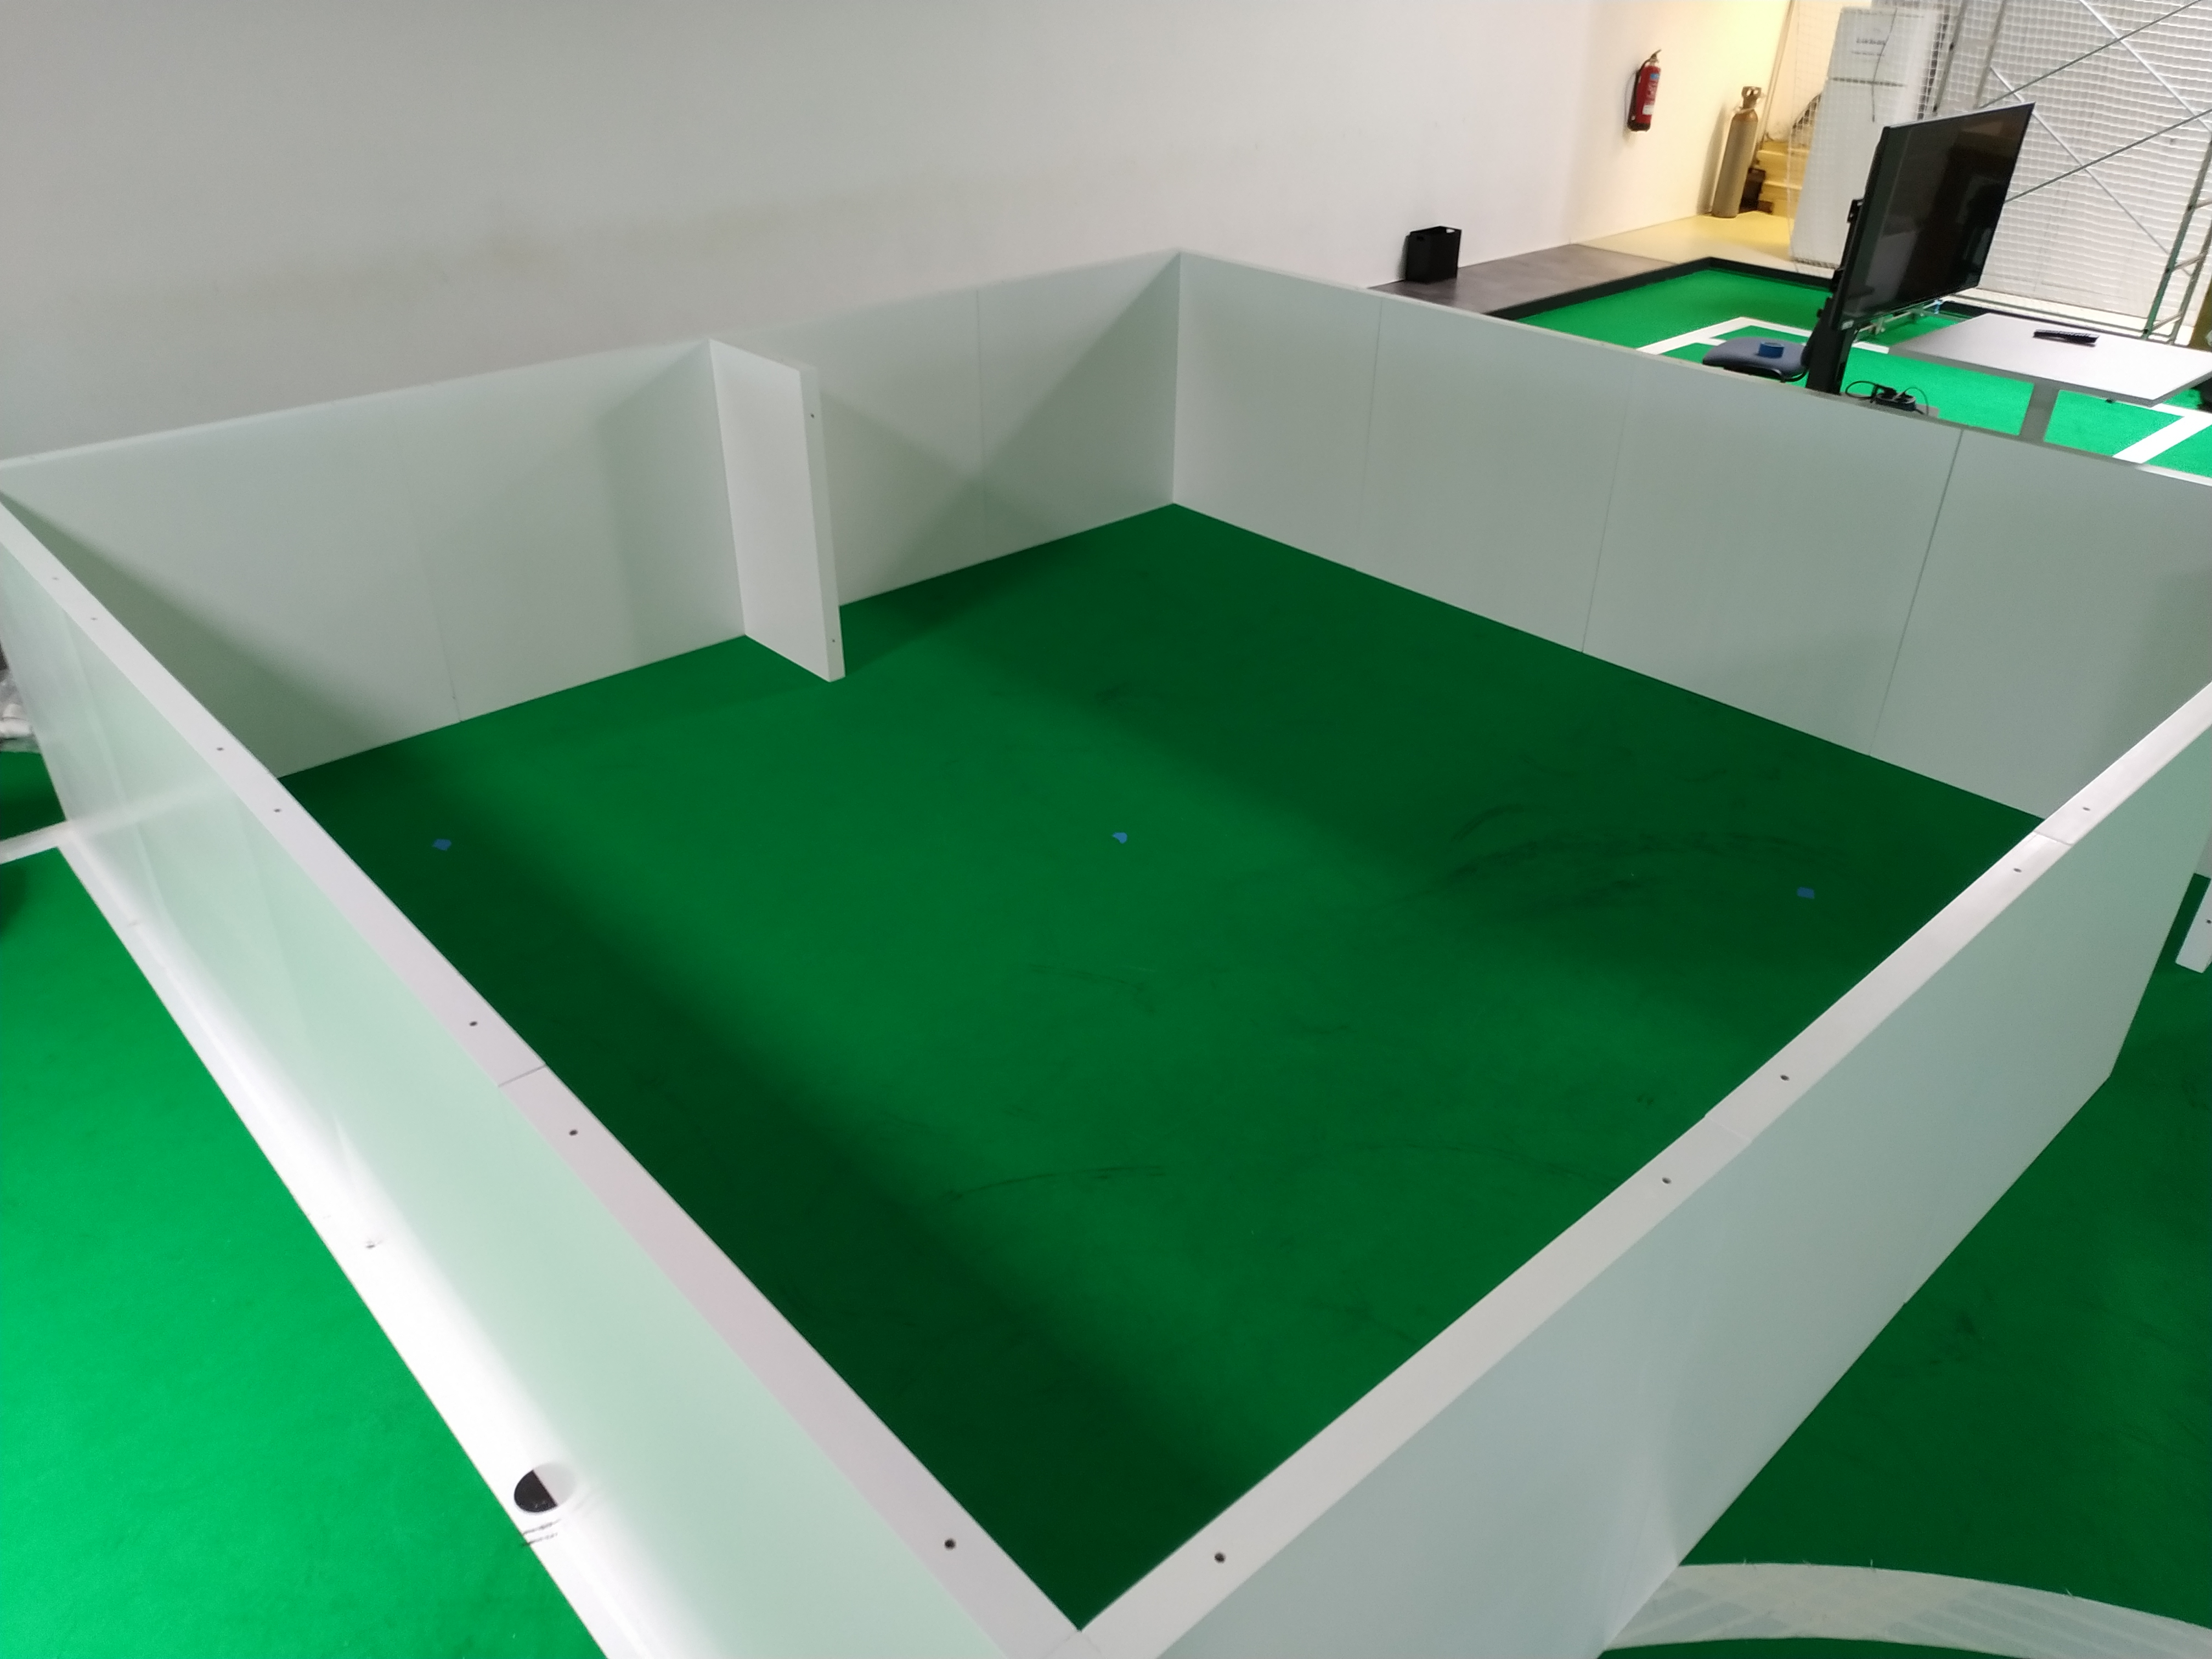
\includegraphics[height=5cm,width=\linewidth]{imgs/chapter5/mapP.jpg}
        \subcaption{Foto of the scenario \cite{robot1}}
        \label{fig:cenario}
    \end{minipage}
    \begin{minipage}[t]{.49\linewidth}
        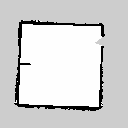
\includegraphics[height=5cm,width=\linewidth]{imgs/chapter5/map.png}
        \subcaption{Map created using \texttt{SLAM} package developed at \ac{IRIS}}
        \label{fig:mapcenario}
    \end{minipage}
    \caption{Scenario Constructed for the experiment}
    \label{fig:setup2}
\end{figure}
This is a 4 by 4 meter squared box with 1 meter high walls with the addition of a half a meter wall in length in the middle. This type of environment optimizes the robots localization system (\ac{AMCL}) as well as make sure we only concentrate with one specific object at a time. Using a \texttt{\ac{SLAM}} package developed here at \ac{IRIS} a map is first created (Figure \ref{fig:mapcenario}) that will later be used for localization purposes.

\subsection{Experimental setup}
With the described scenario we setup the robots goal to make five loops between two goals, position A and B, positioning in between the route an obstacle as illustrated in  Figure \ref{fig:exp}. 
\begin{figure}[ht!]
\centerline{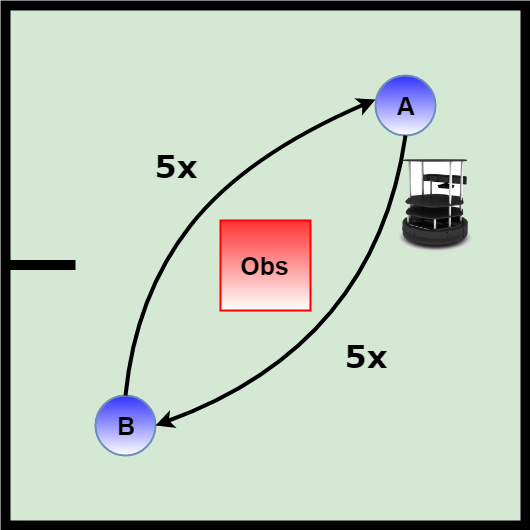
\includegraphics [width=0.5 \textwidth]{imgs/chapter5/exp.png}}
\caption[Demonstration of the course of test]{Demonstration of the course of test, the robot will go back and forth from position A to position B 5 times while  trying to avoid the obstacle in the middle}
\label{fig:exp}
\end{figure}

If the obstacle detection system fails then the robot should collide with said object, if it succeeds the robot should go around the object leaving in between a relatively safe distance. 
%The test was made using the \ac{FMCW} radar, the 2D \ac{LiDAR}, and the fusion of both for different types of objects. 
The  navigation data was recorded in a rosbag file in order to be analyzed later.

The list of objects used as obstacles are displayed in Fig. \ref{fig:obstacles}.
\begin{figure}[h!]
  \centering
  \begin{subfigure}[b]{0.3\linewidth}
    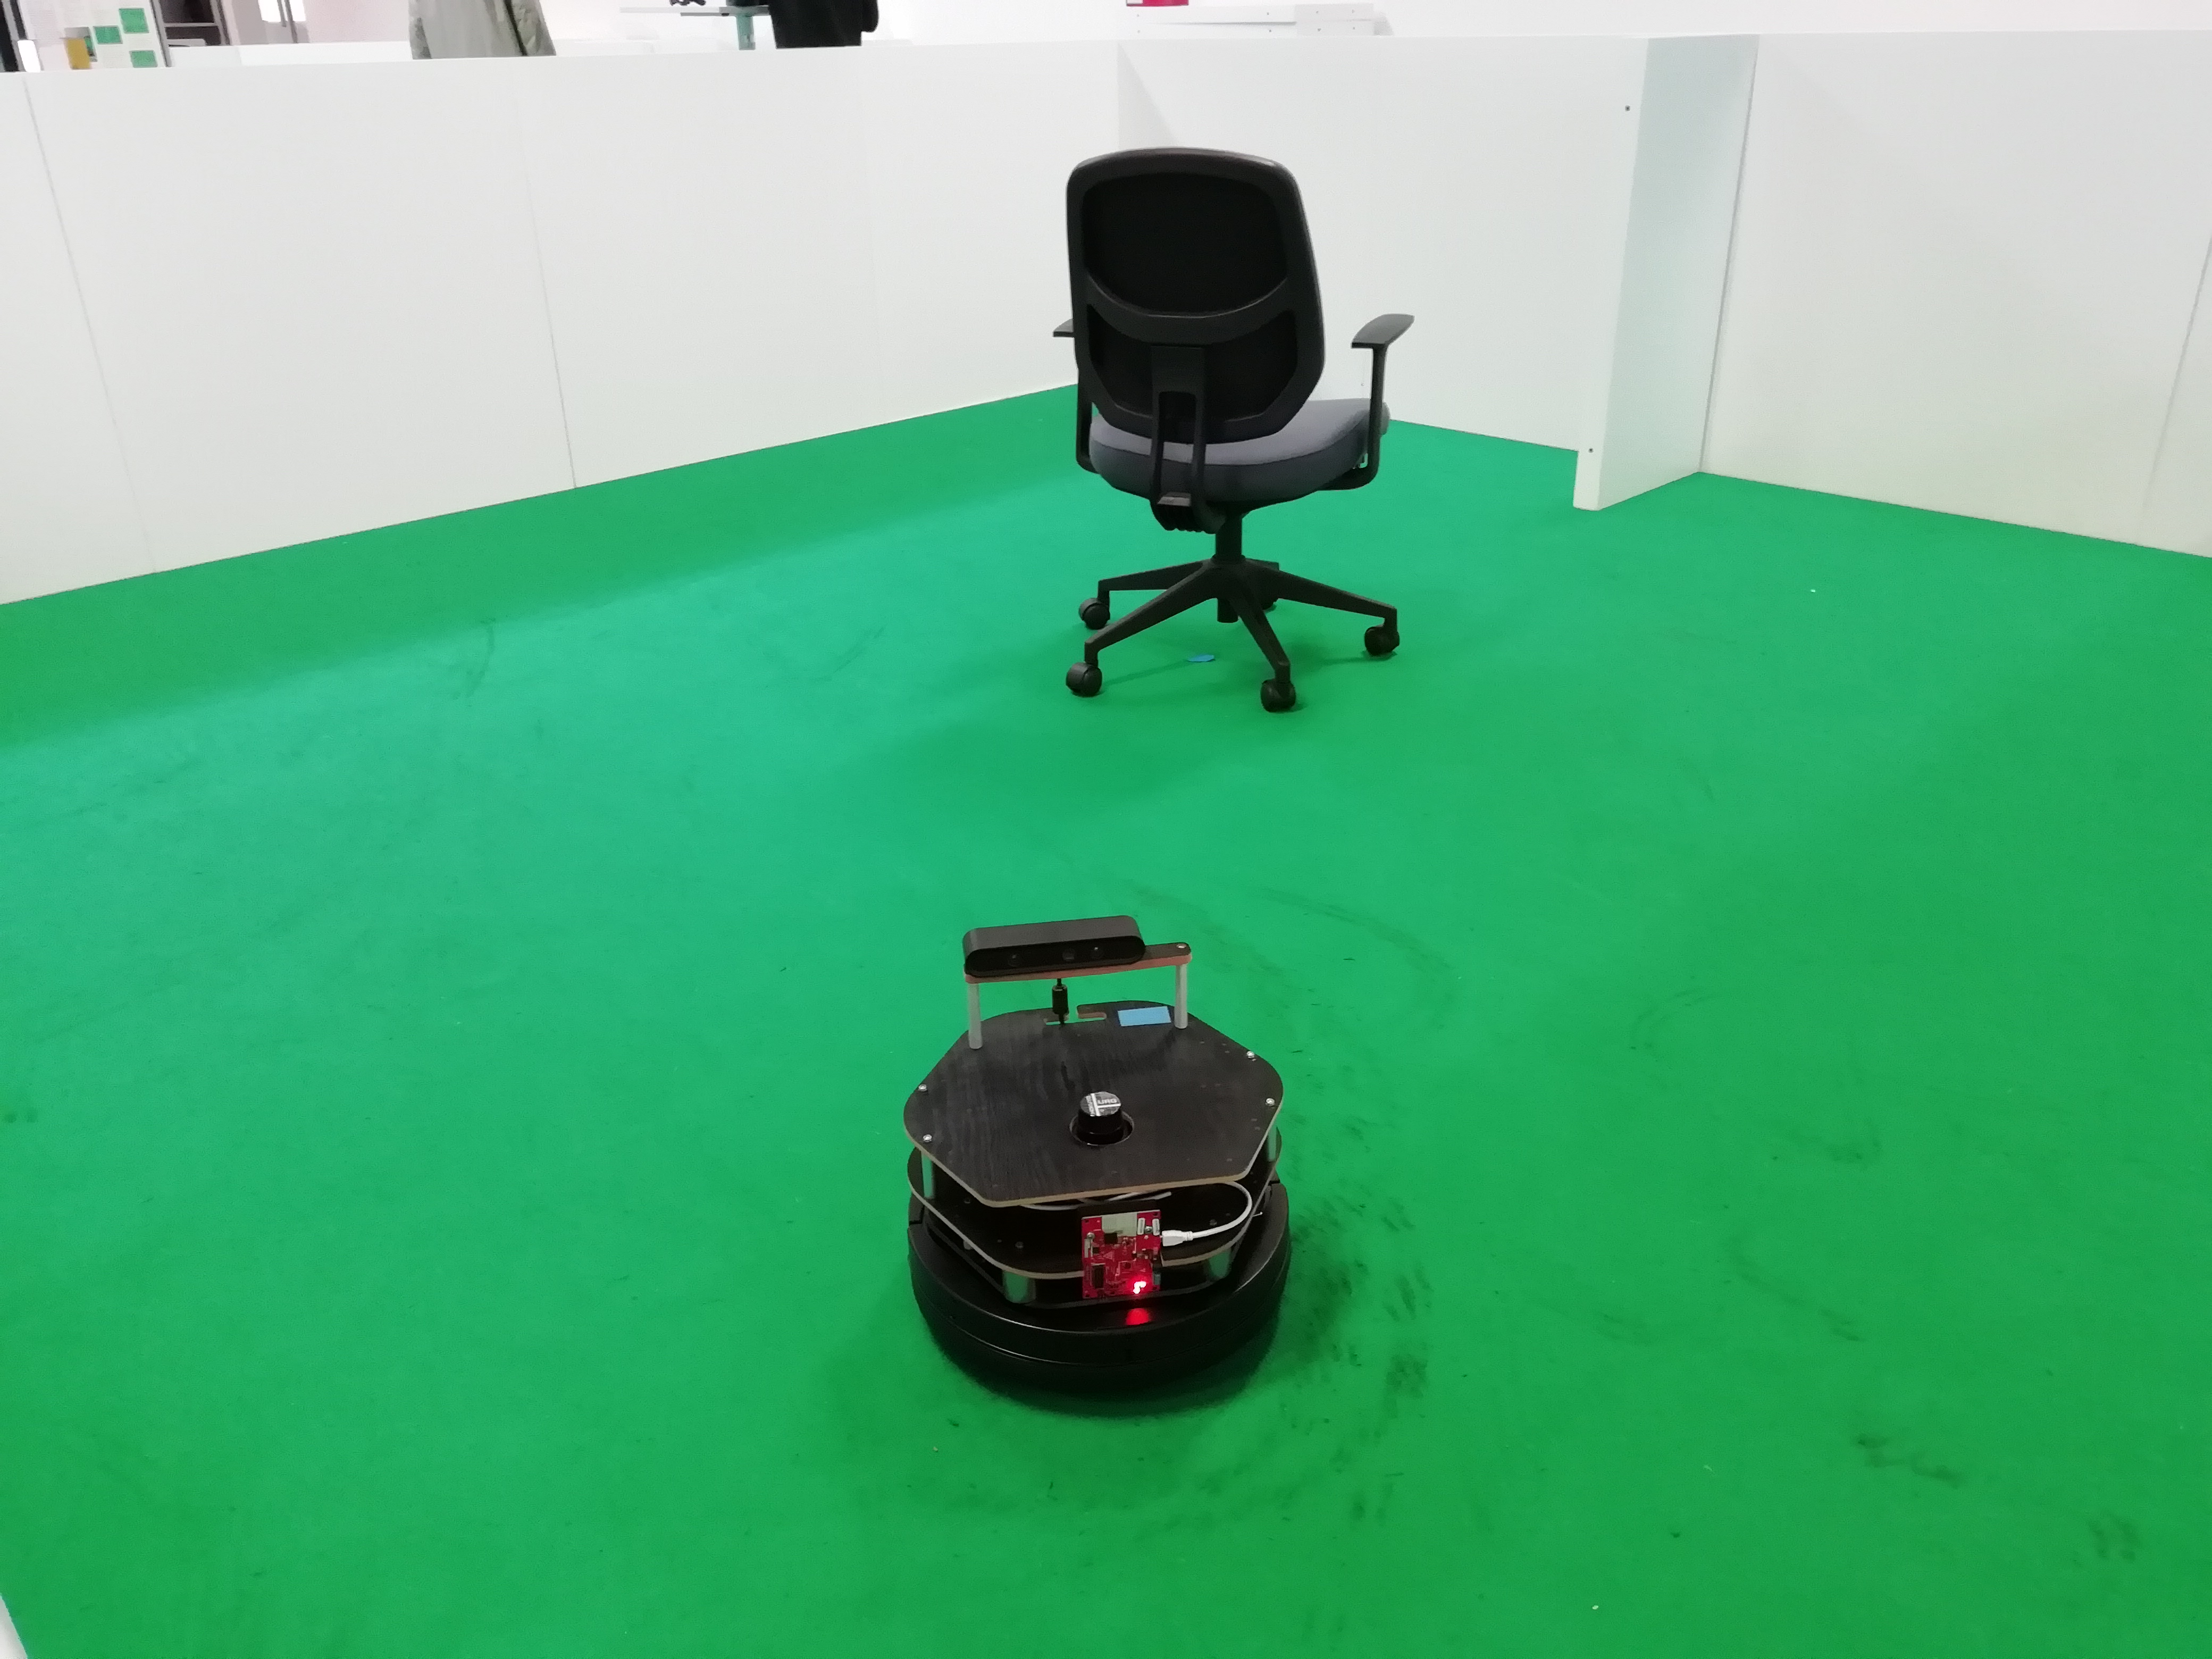
\includegraphics[width=\linewidth]{imgs/chapter5/wchair.jpg}
     \caption{Office chair}
     \label{fig::wchair}
  \end{subfigure}
  \begin{subfigure}[b]{0.3\linewidth}
    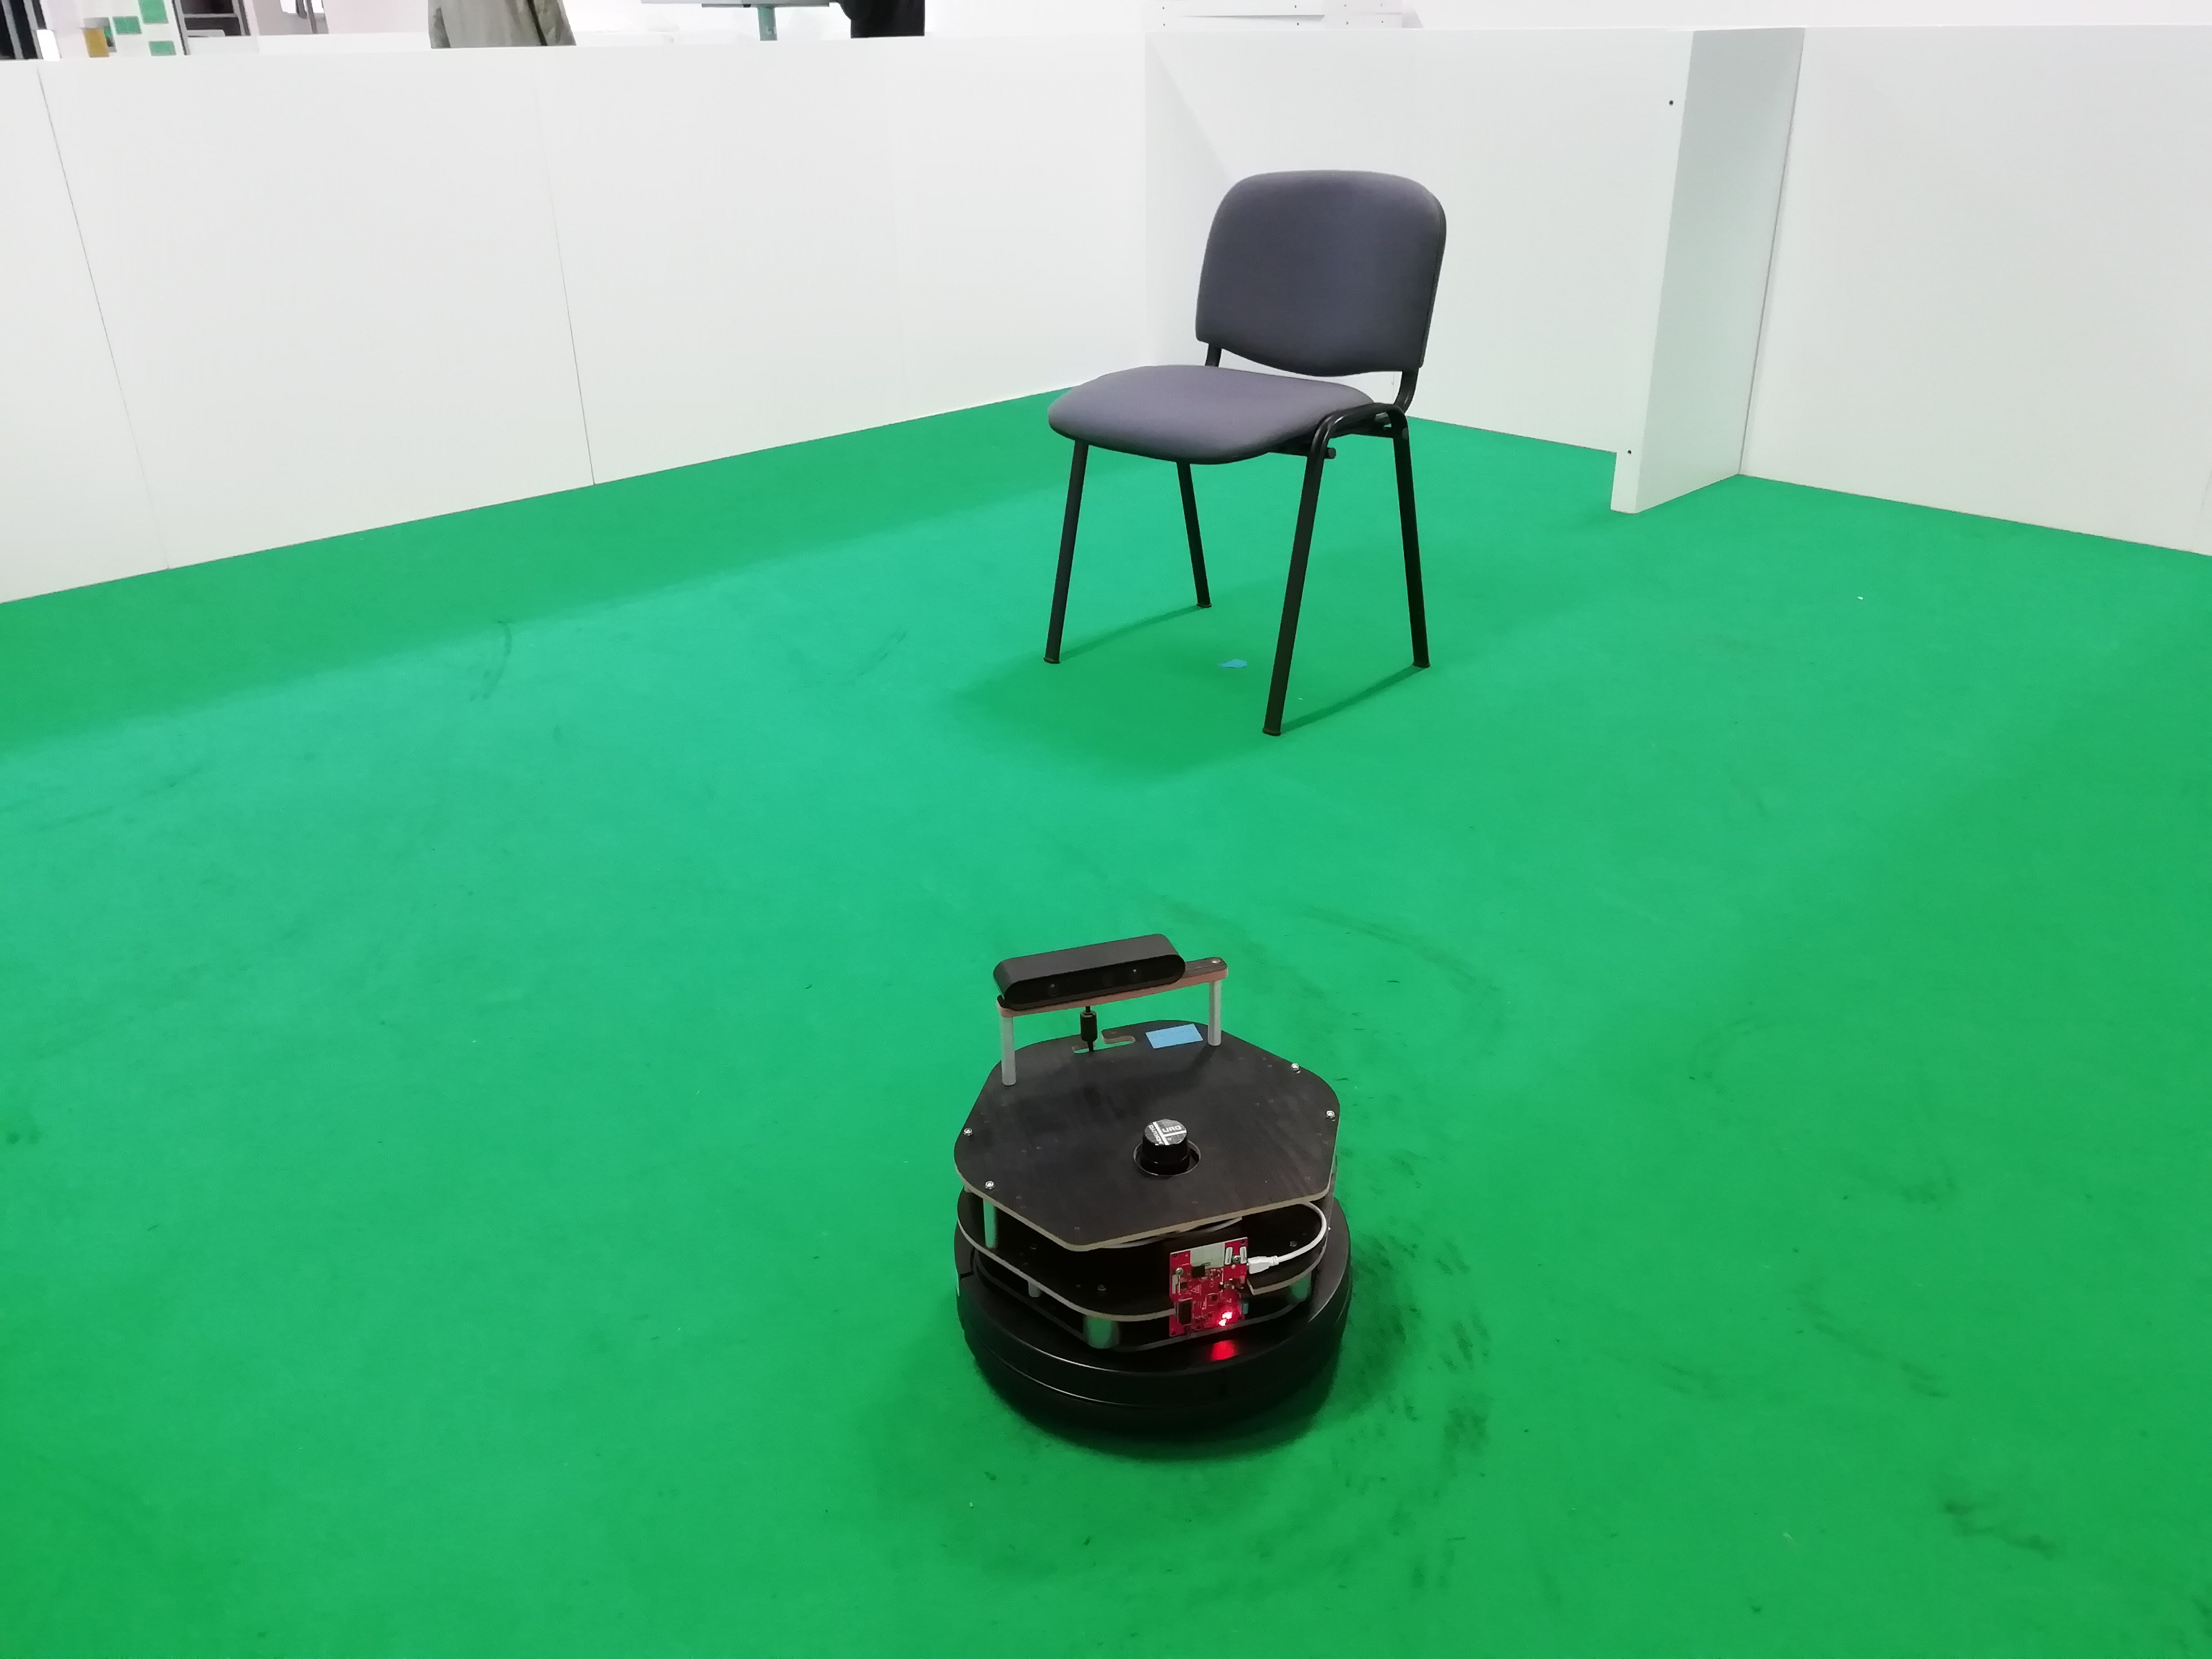
\includegraphics[width=\linewidth]{imgs/chapter5/nchair.jpg}
    \caption{Four legged chair}
    \label{fig::nchair}
  \end{subfigure}
  \begin{subfigure}[b]{0.3\linewidth}
    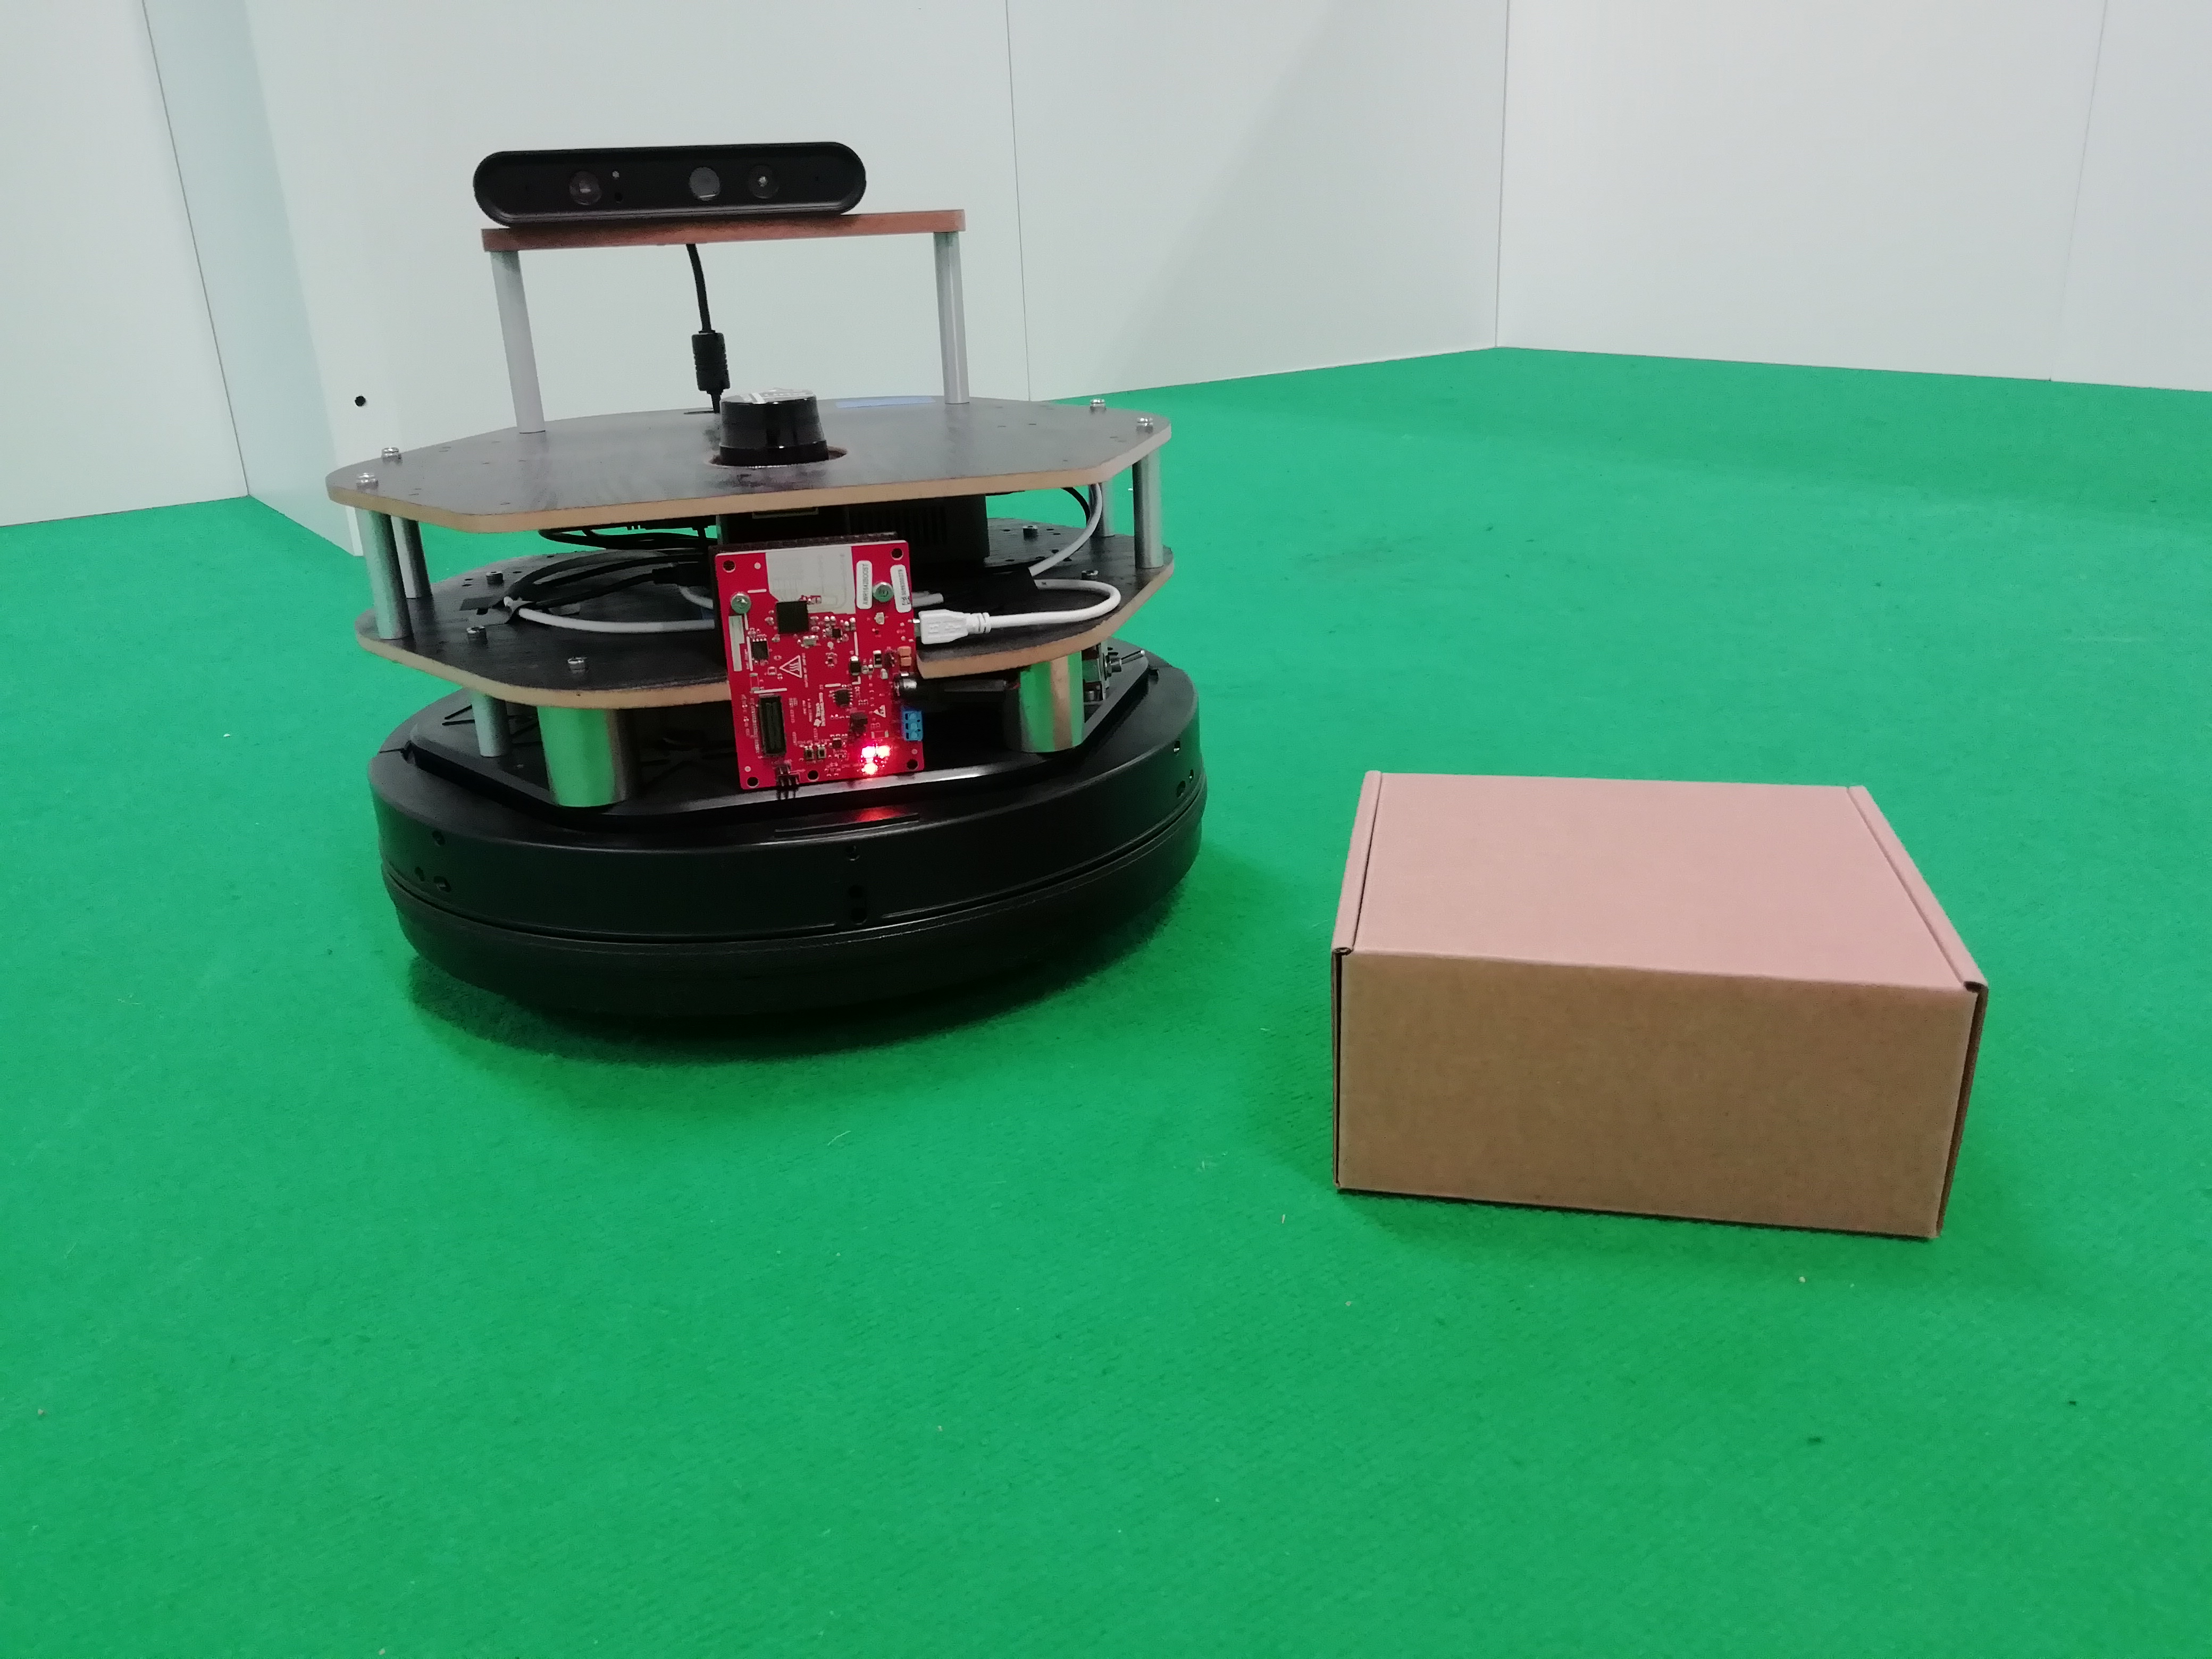
\includegraphics[width=\linewidth]{imgs/chapter5/box.jpg}
    \caption{Low height box}
    \label{fig::box}
  \end{subfigure}
  \begin{subfigure}[b]{0.3\linewidth}
    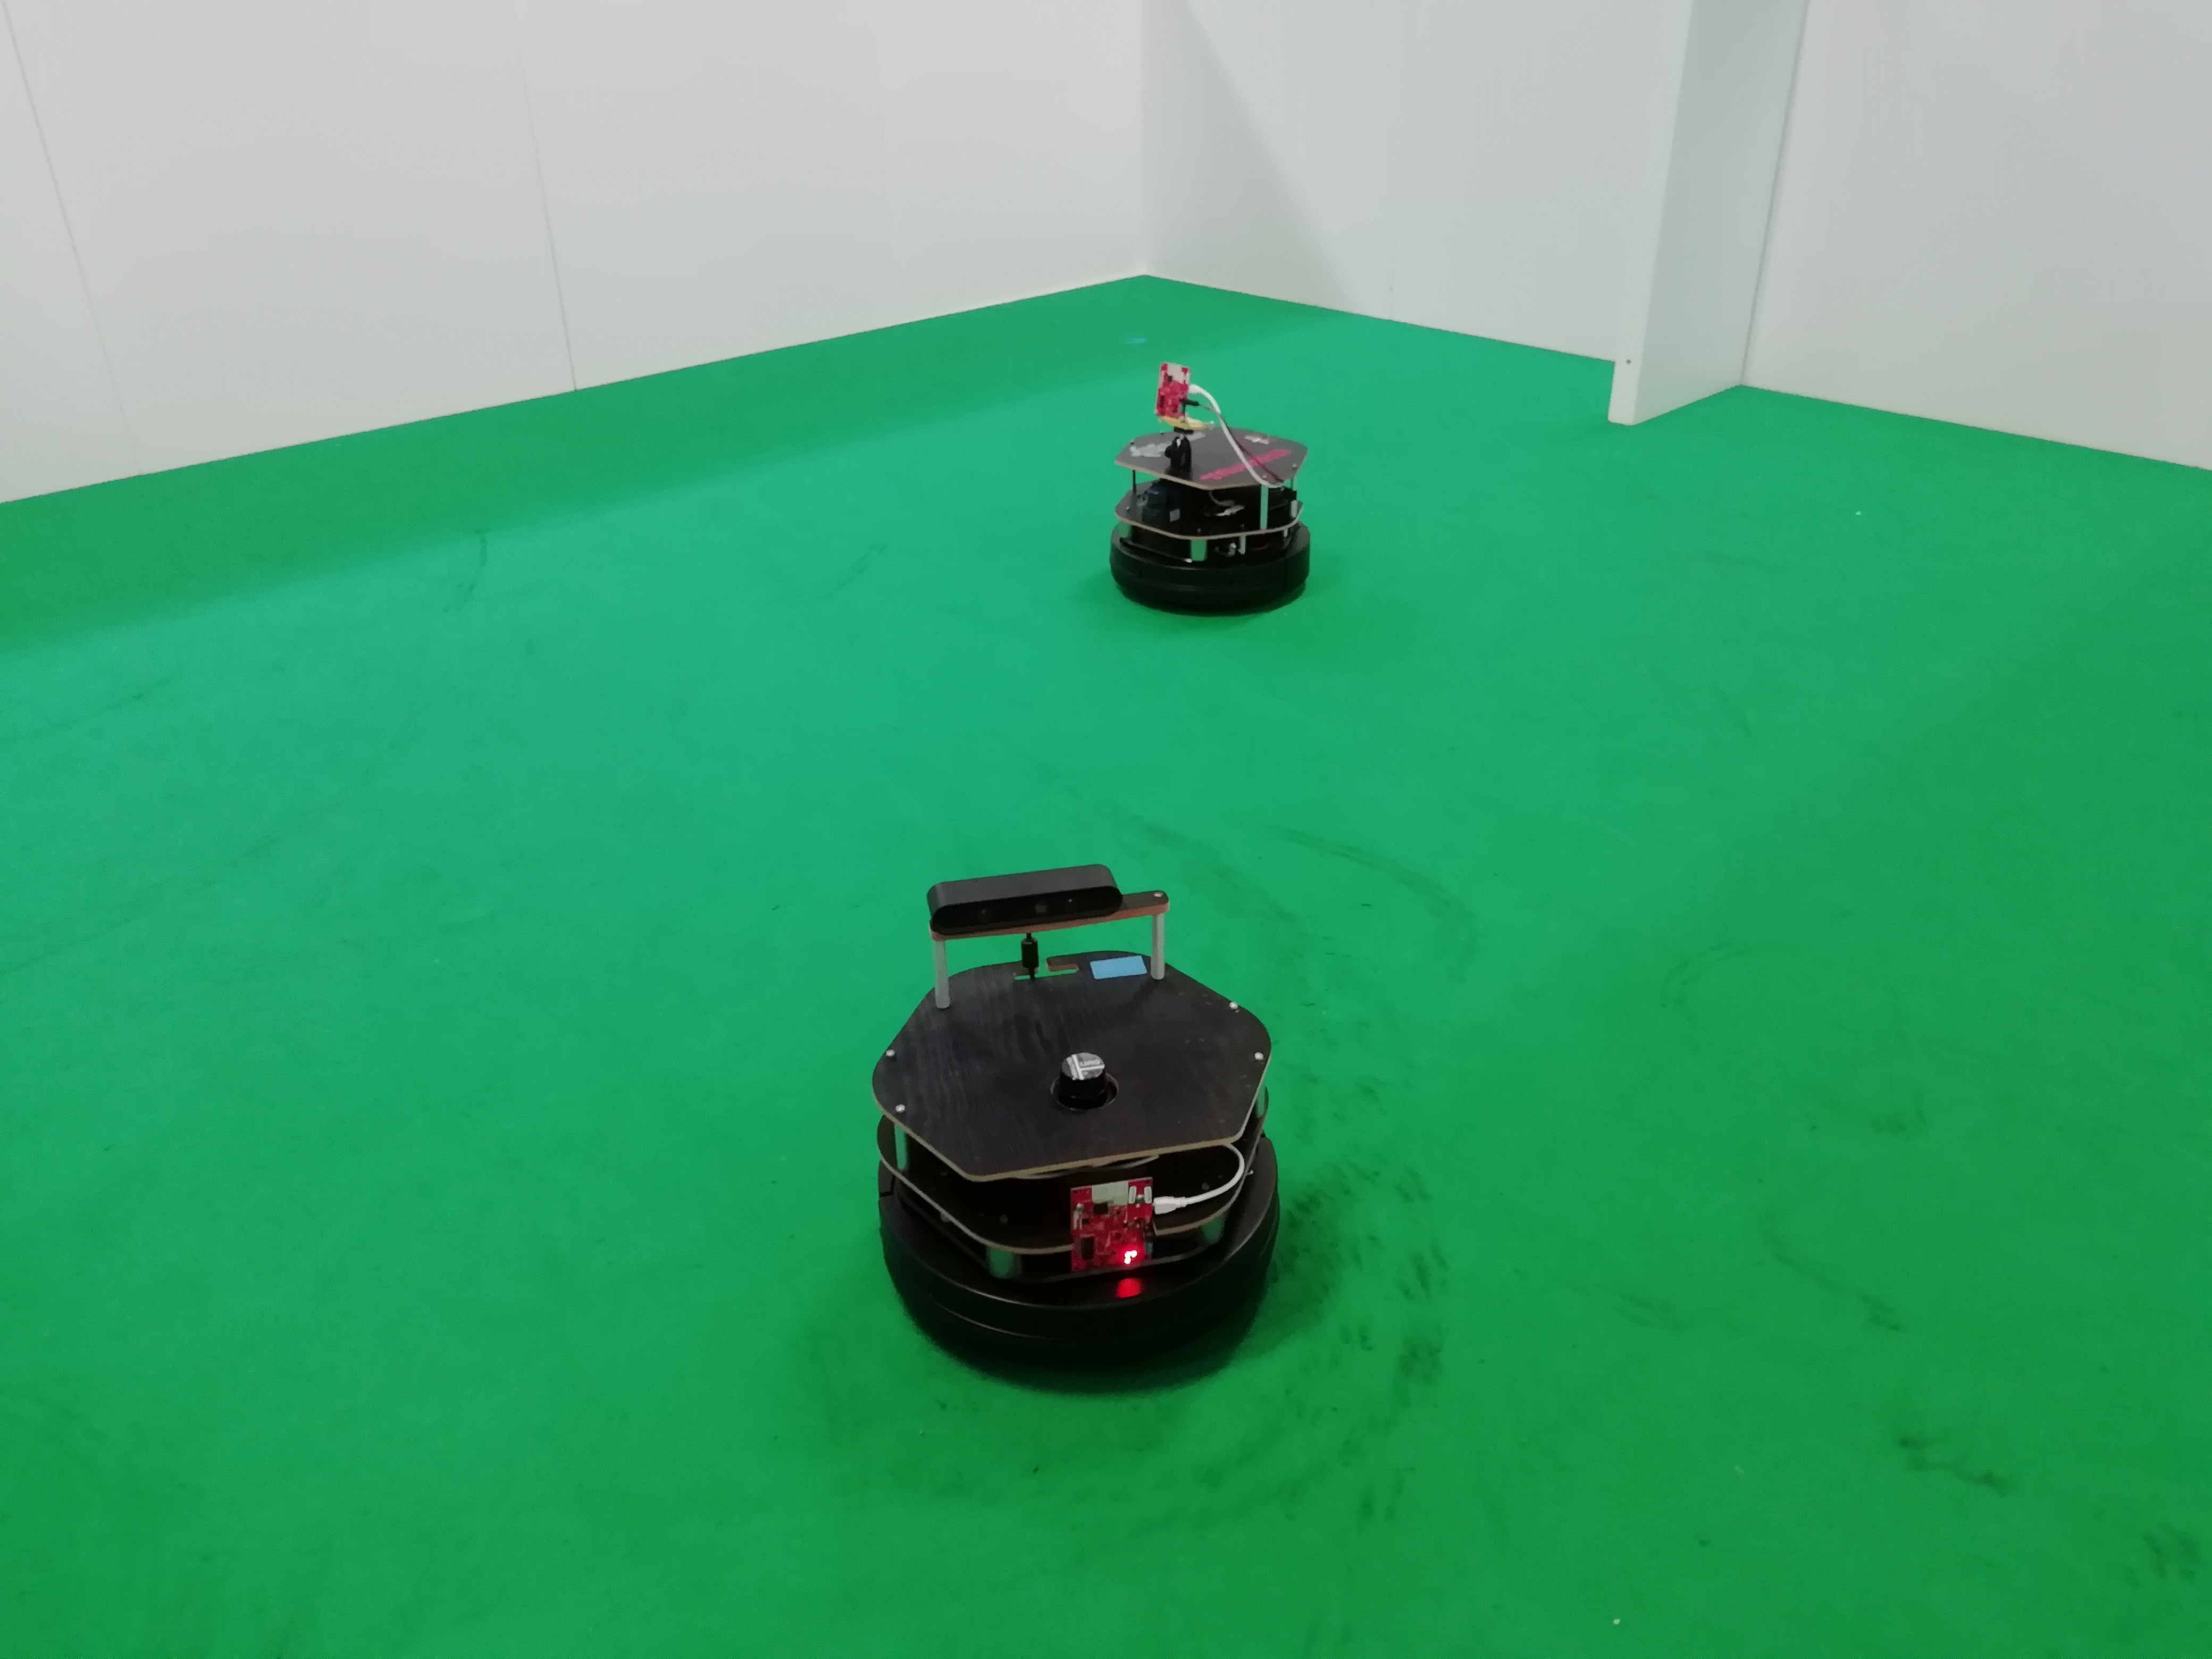
\includegraphics[width=\linewidth]{imgs/chapter5/robot.jpg}
    \caption{Another turtlebot}
    \label{fig::robot}
  \end{subfigure}
  \begin{subfigure}[b]{0.3\linewidth}
    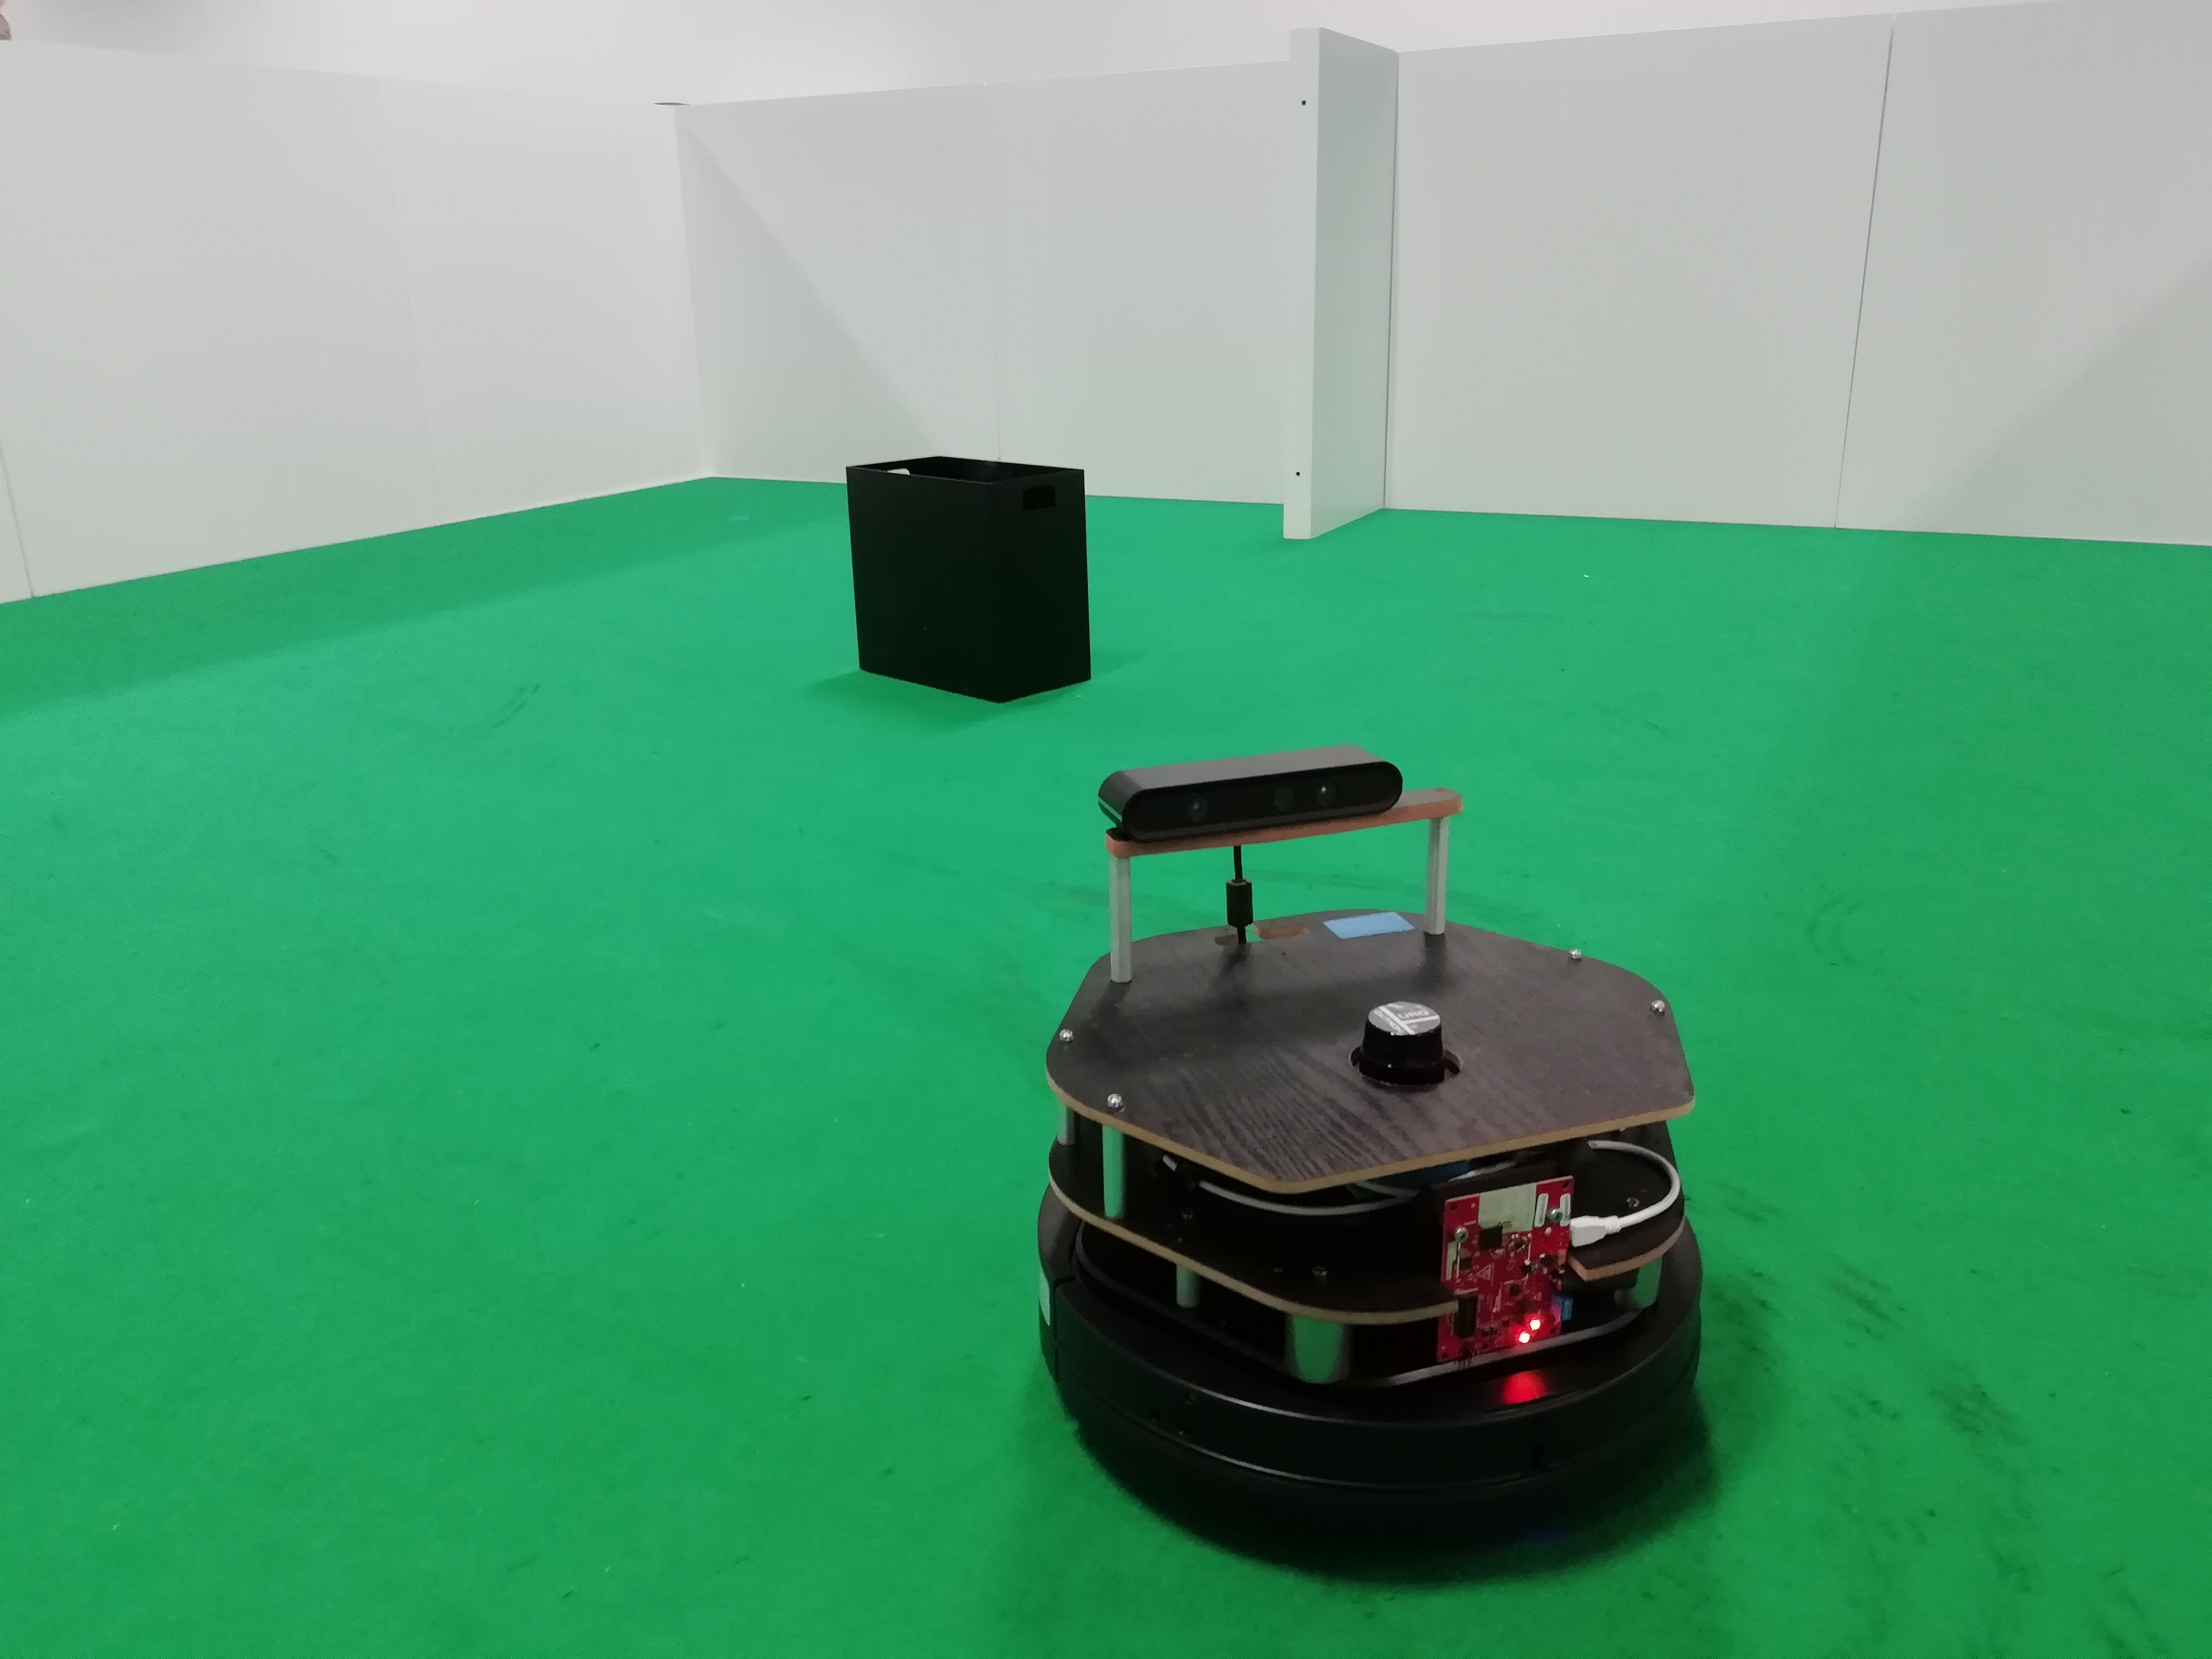
\includegraphics[width=\linewidth]{imgs/chapter5/garbage.jpg}
    \caption{Garbage Bin}
    \label{fig::garbage}
  \end{subfigure}
  \begin{subfigure}[b]{0.3\linewidth}
    \includegraphics[width=\linewidth]{imgs/chapter5/glass.jpg}
    \caption{Acrylic tube}
    \label{fig::tube}
  \end{subfigure}
  \caption{Different obstacles used for the controlled test}
  \label{fig:obstacles}
\end{figure}

\subsection{Results}
In this section we show the results of how the robot performed in avoiding the previous obstacles using different type of sensor sources (\ac{FMCW} radar, the 2D \ac{LiDAR} and both).

\subsubsection{Office Chair}







\subsubsection*{\ac{LiDAR}}
In the \ac{LiDAR}'s case  the robot completely disregarded the chair going in a straight line and pushing it until it was away from the experimental setup has shown in Figure \ref{fig:wchairLF}.

\begin{figure}[h!]
  \centering
  \begin{subfigure}[b]{0.49\linewidth}
    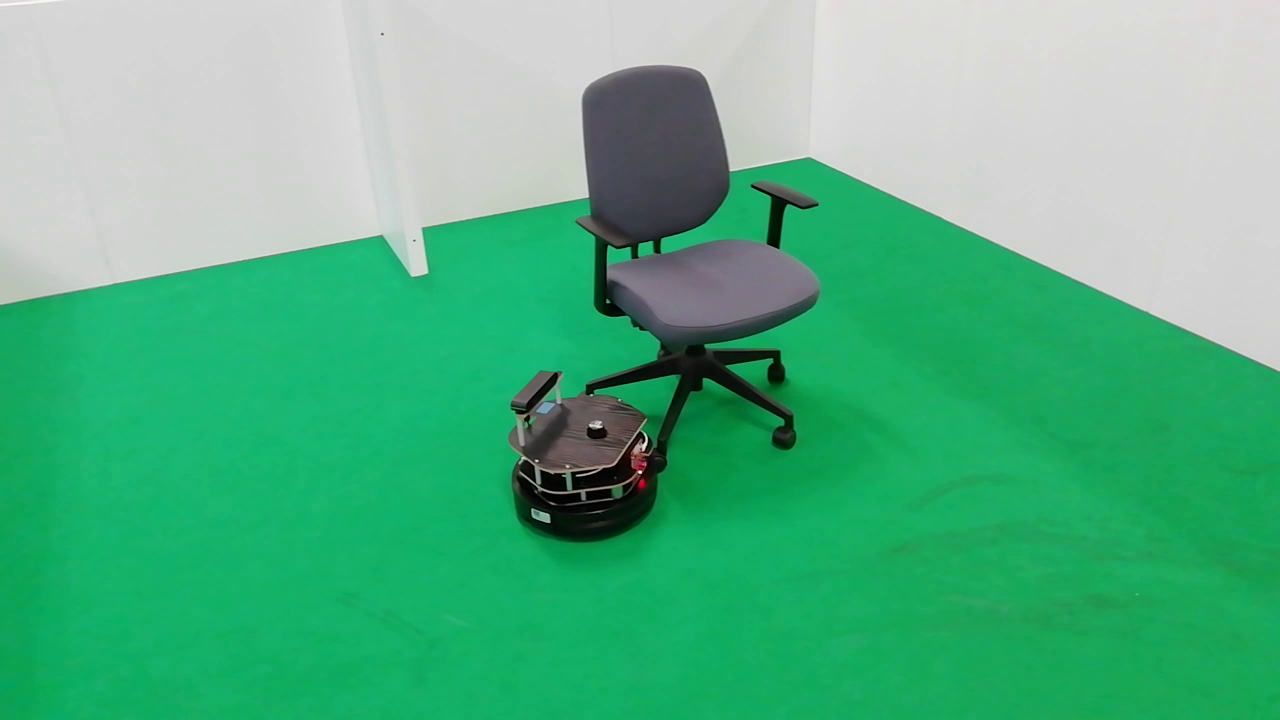
\includegraphics[width=\linewidth]{imgs/chapter5/wchairLF.png}
     \caption{Robot collision with office chair number 1}
     \label{fig::wchairLF1}
  \end{subfigure}
  \begin{subfigure}[b]{0.49\linewidth}
    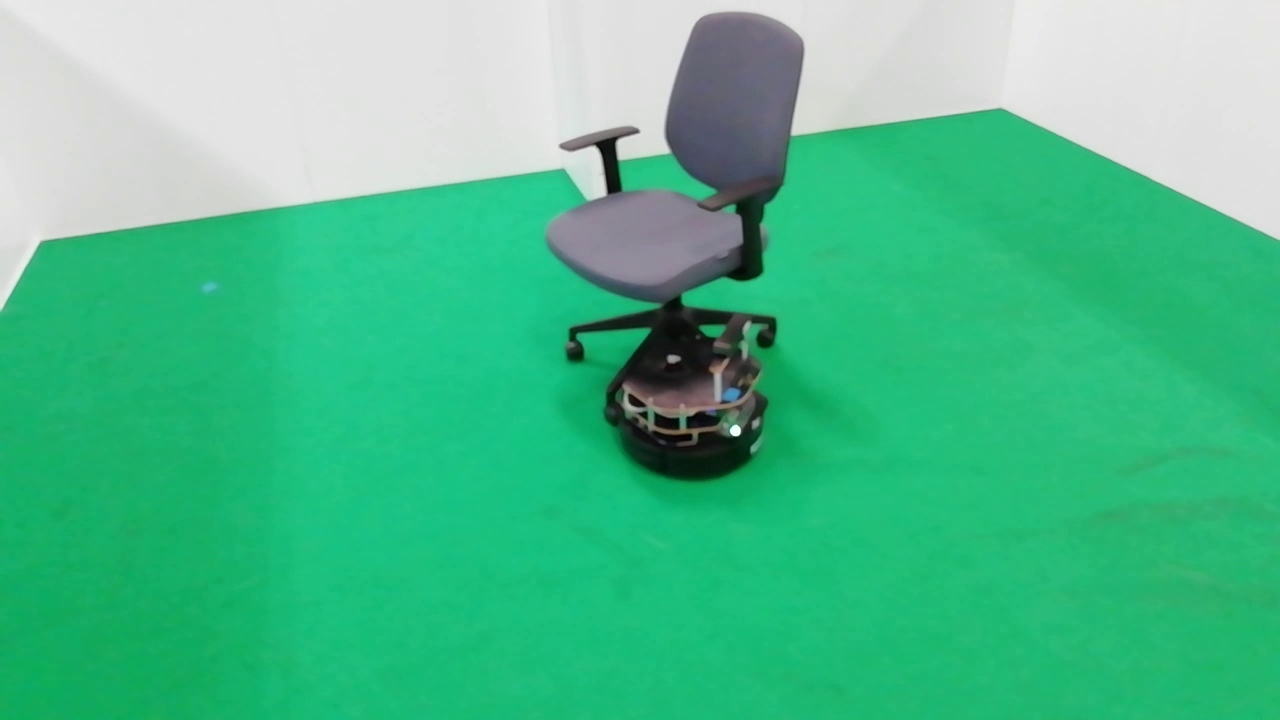
\includegraphics[width=\linewidth]{imgs/chapter5/wchairLF2.png}
    \caption{Robot collision with office chair number 2}
    \label{fig::wchairLF2}
  \end{subfigure}
  \caption{Robot colliding multiple times with office chair}
  \label{fig:wchairLF}
\end{figure}






This was due to the 2D \ac{LiDAR} only detecting the leg of the chair and not the wheels. This means that the robot only perceived a single point as being occupied and not the full area of the chair. Although the inflation layer  might correct this error in some cases, since the detection is so late the robot still was unable to avoid it.

\subsubsection*{\ac{FMCW} \ac{radar}}
However with the \ac{FMCW} radar the chair is detected almost immediately, this makes the global planner and motion controller to be able to adjust in a very comfortable way and with it the robot is able to avoid collision. Figure \ref{fig:wchairRS} shows some instances of the first experiment. Although the detected space that the chair is occupying has some mismatch, the early detection makes up for it. However since the radar has small field of view (120 degrees) the robot might not detect the obstacle when it is passing by it which in this case lead to it scraping by the chair one time.

\begin{figure}[h!]
  \centering
  \begin{subfigure}[b]{0.49\linewidth}
    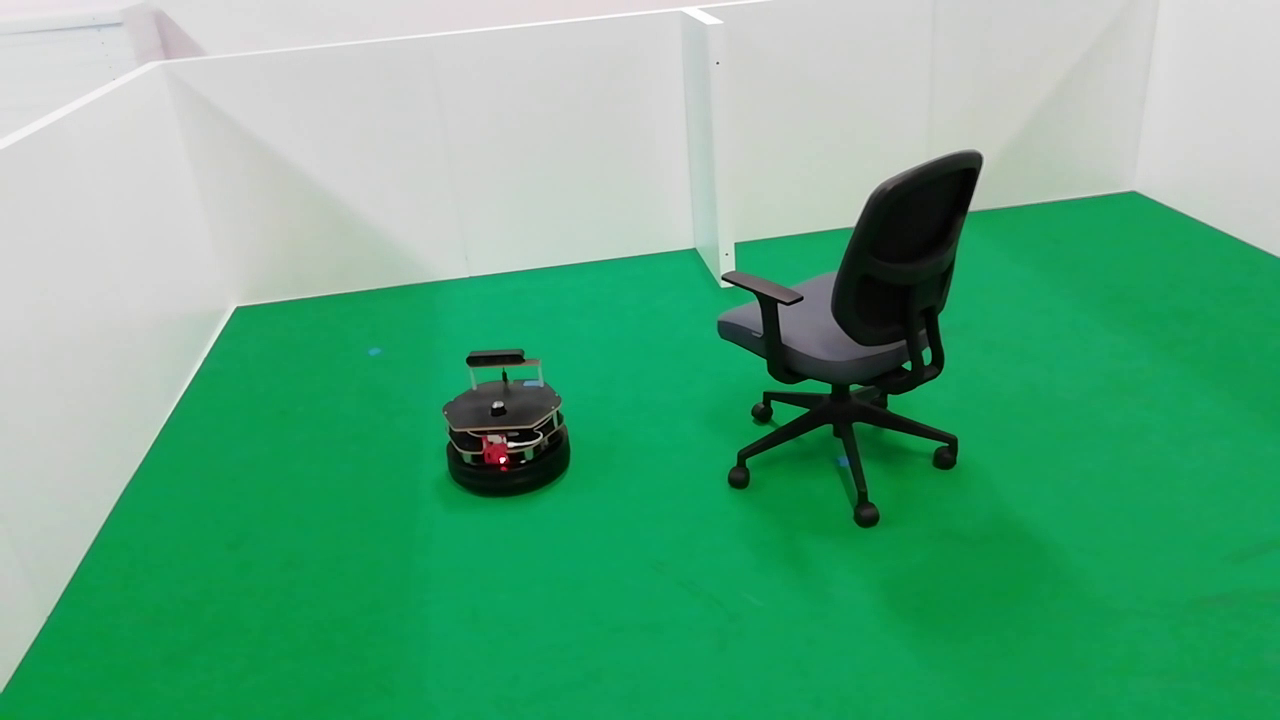
\includegraphics[width=\linewidth]{imgs/chapter5/wchairRS.png}
     \caption{Robot avoiding office chair number 1}
     \label{fig::wchairRS1}
  \end{subfigure}
  \begin{subfigure}[b]{0.49\linewidth}
    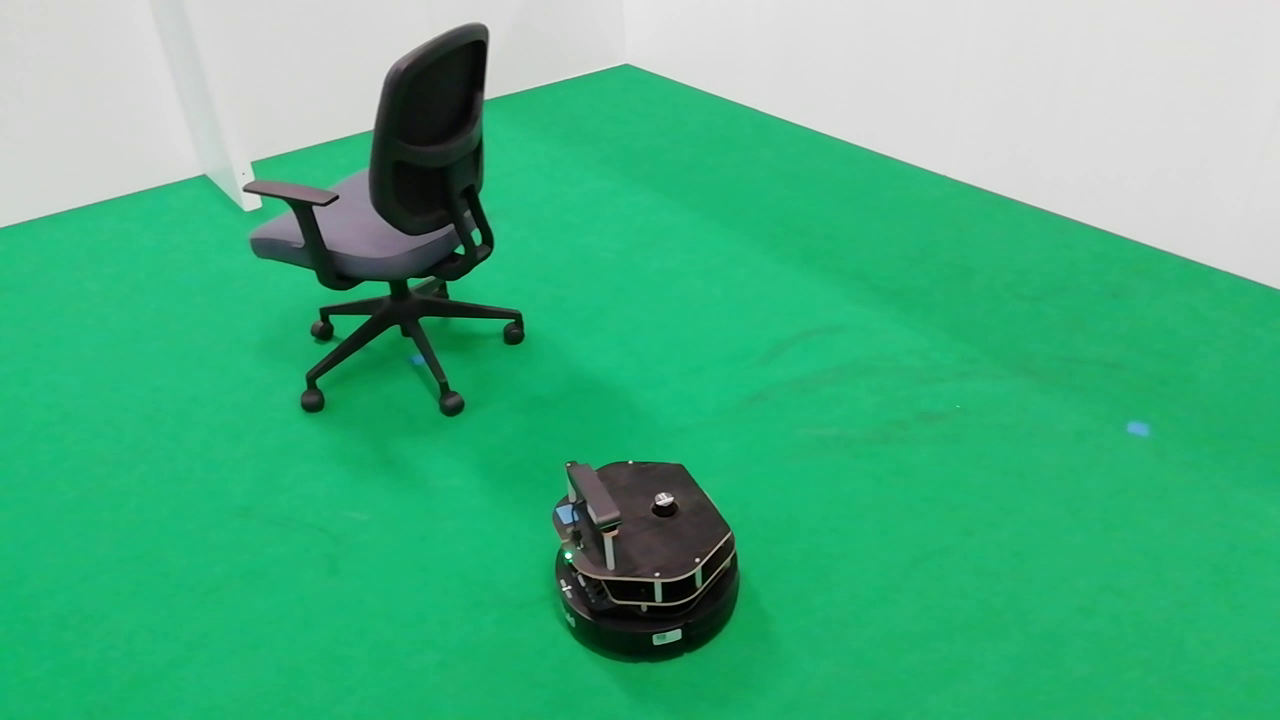
\includegraphics[width=\linewidth]{imgs/chapter5/wchairRS2.png}
    \caption{Robot avoiding office chair number 2}
    \label{fig::wchairRS2}
  \end{subfigure}
  \caption{Robot avoiding with office chair}
  \label{fig:wchairRS}
\end{figure}

\subsubsection*{Robot Trajectory}
Figure \ref{fig:traj1} shows the robot trajectory in the \ac{LiDAR} and the \ac{FMCW} radar case aswell an aproximation of the of the invalid space the  center of the robot can not go through in dimmed red. As we can see the robot flat out ignores the obstacle with \ac{LiDAR} while in the \ac{FMCW} \ac{radar} case it narrowly avoids it at all times.
\begin{figure}[ht!]
\centerline{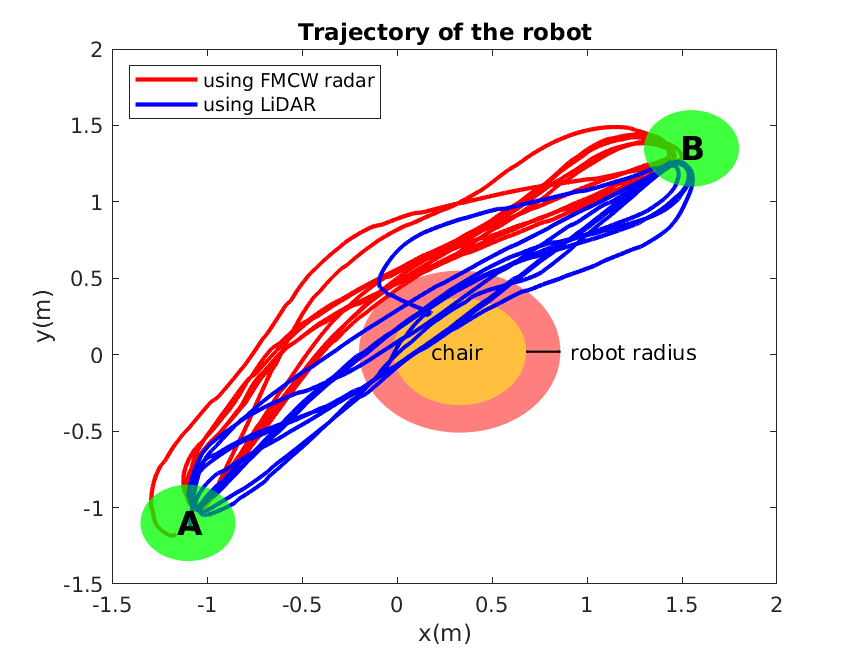
\includegraphics [width=0.7 \textwidth]{imgs/chapter5/traj1.png}}
\caption{Trajectory of the robot for the office chair's case}
\label{fig:traj1}
\end{figure}


\subsubsection{Four Legged Chair}
\subsubsection*{LiDAR}
Using \ac{LiDAR} the robot did not succeed in producing a safe trajectory.

First off it went in a straight line just as the previous case almost hitting  the legs of the chair. However when it got to close to it, it came to a halt and kept oscillating for a long time until it either collided with the leg or scrapping by it. This was again due to the \ac{LiDAR} only detecting this type of obstacle at small distances. This behavior repeated itself throughout the task, leading to the chair being pushed several times. Figure \ref{fig:nchairLF} shows two instances where the robot gets stuck near the chair. This type of behavior is indicative that the robot's motion controller is stuck in local minimum, in other words computing a safe trajectory around the obstacle is countered by its force to follow the goal and path.
\begin{figure}[h!]
  \centering
  \begin{subfigure}[b]{0.49\linewidth}
    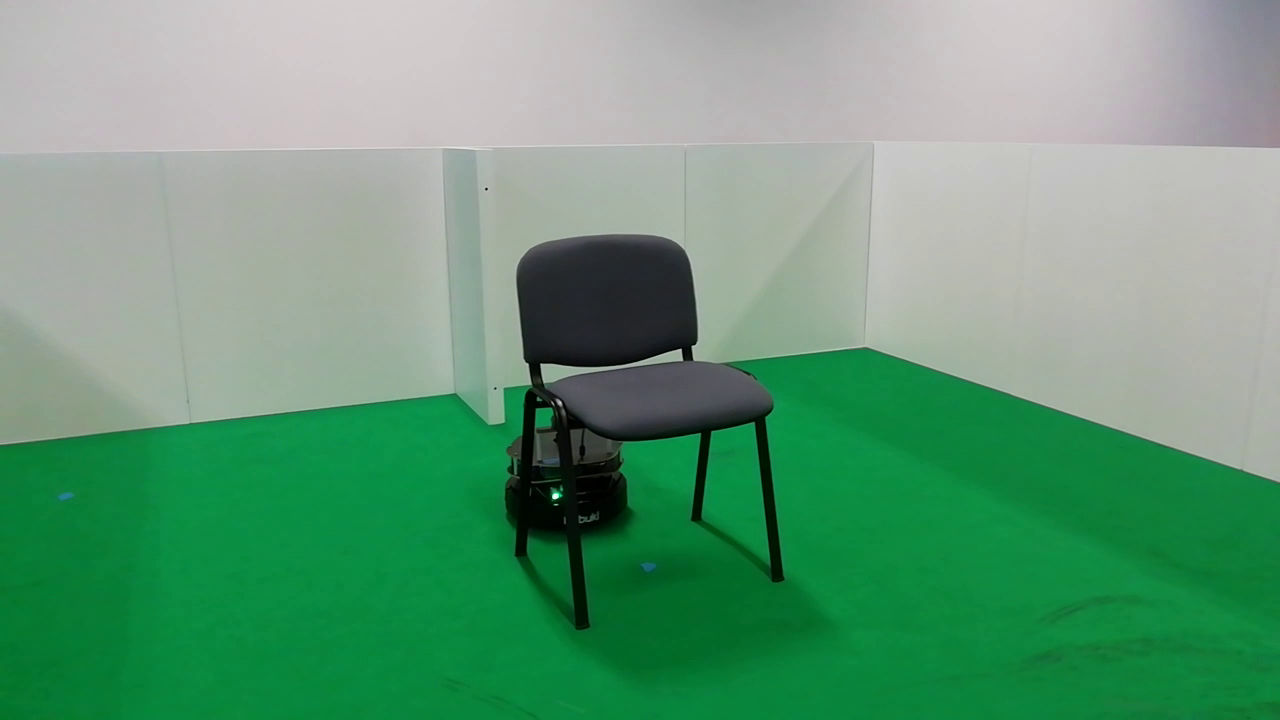
\includegraphics[width=\linewidth]{imgs/chapter5/nchairLF.png}
     \caption{Robot getting stuck in chair number 1}
     \label{fig::nchairLF1}
  \end{subfigure}
  \begin{subfigure}[b]{0.49\linewidth}
    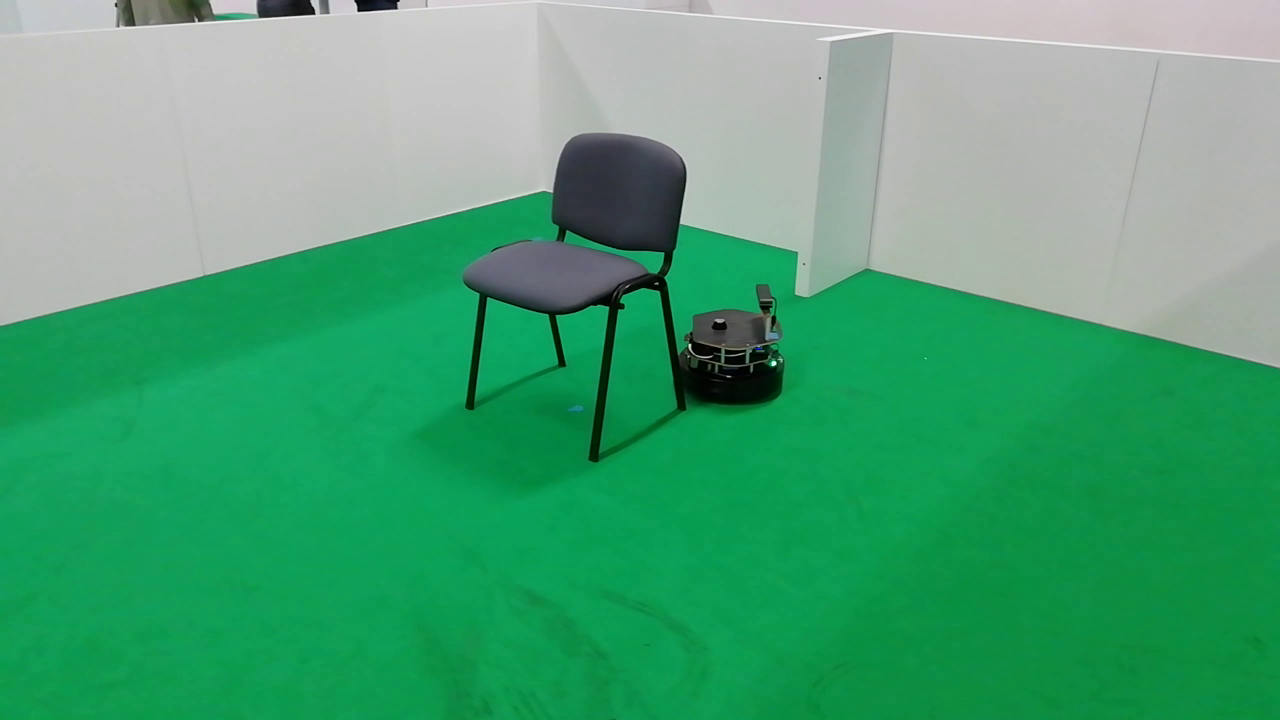
\includegraphics[width=\linewidth]{imgs/chapter5/nchairLF2.png}
    \caption{Robot getting stuck in chair number 2}
    \label{fig::nchairLF2}
  \end{subfigure}
  \caption{Robot avoiding getting stuck in four legged chair}
  \label{fig:nchairLF}
\end{figure}

\subsubsection*{FMCW radar}
Using the \ac{FMCW} radar proved to be much better with the robot safely circumventing around the chair with safe distance for all duration of the task. Figure \ref{fig:nchairRS} shows two instances of the turtlebot avoiding the chair in at a safe distance.
\begin{figure}[h!]
  \centering
  \begin{subfigure}[b]{0.49\linewidth}
    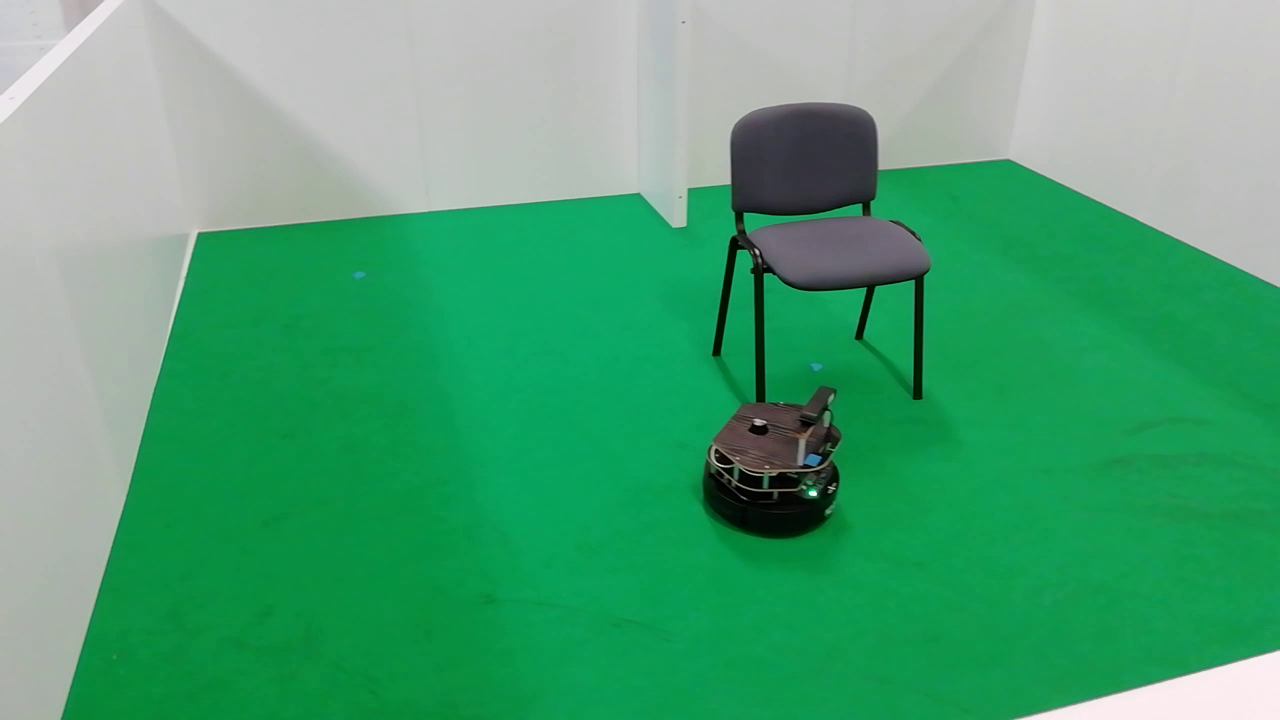
\includegraphics[width=\linewidth]{imgs/chapter5/nchairRS.png}
     \caption{Robot avoiding four legged chair number 1}
     \label{fig::nchairRS1}
  \end{subfigure}
  \begin{subfigure}[b]{0.49\linewidth}
    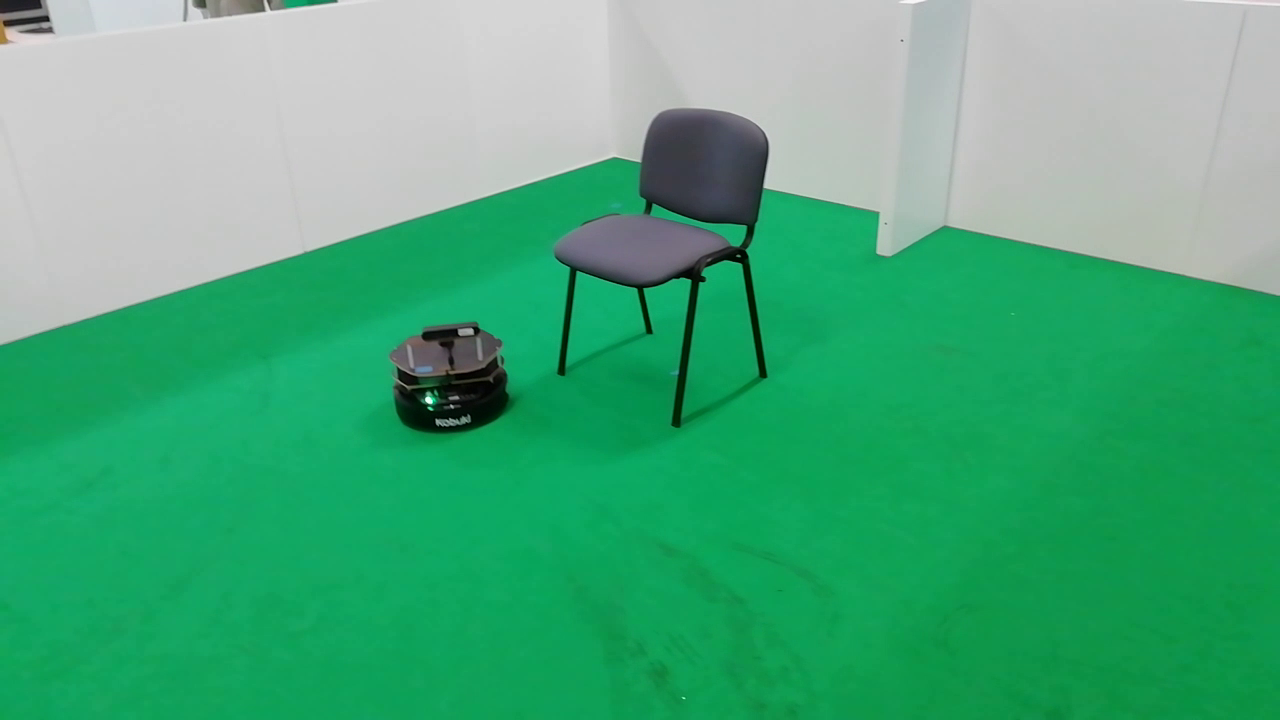
\includegraphics[width=\linewidth]{imgs/chapter5/nchairRS2.png}
    \caption{Robot avoiding four legged chair number 2}
    \label{fig::nchairRS2}
  \end{subfigure}
  \caption{Robot avoiding the four legged chair}
  \label{fig:nchairRS}
\end{figure}

Analysing the data we see that when the robot is facing it it detects almost all legs immediately. 
%PUT RVIZ PICTURE?
This makes it so the robot is aware of it at all times and planning around it.


\subsubsection*{Robot Trajectory}

Figure \ref{fig:traj2} shows the trajectory of the robot for the \ac{LiDAR} and \ac{FMCW} \ac{radar} and an approximate position of the invalid space the four legs of the chair create coloured in dimmed red. The center of the robot should not passtrough this area since it will lead to collision. As we can see the trajectory  produced in the \ac{FMCW} radar case is much less susceptible to the object than in the \ac{LiDAR} case. 
\begin{figure}[ht!]
\centerline{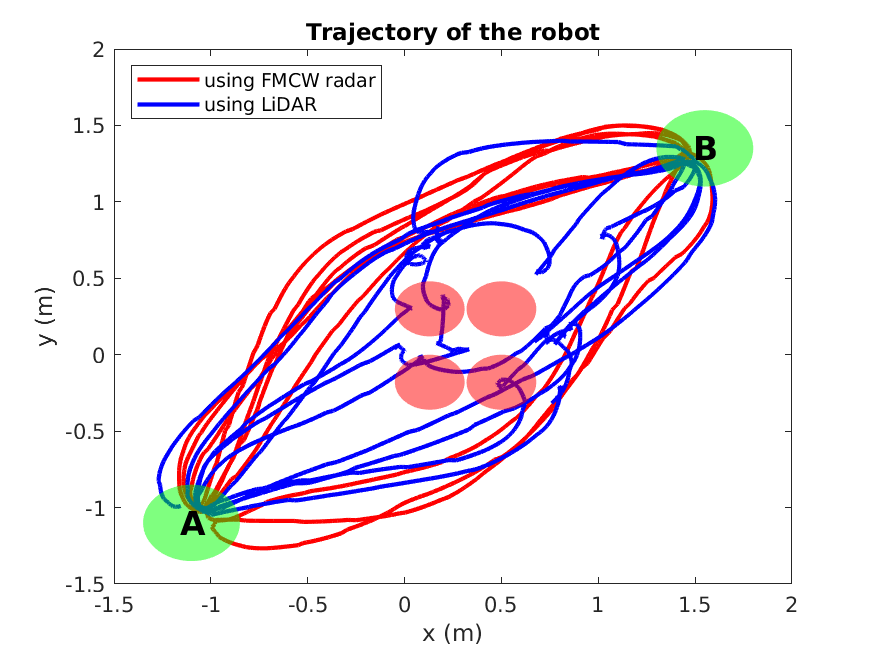
\includegraphics [width=0.7 \textwidth]{imgs/chapter5/traj2.png}}
\caption{Trajectory of the robot for the four-legged chair's case}
\label{fig:traj2}
\end{figure}

\subsubsection{Garbage Bin}

\subsubsection*{LiDAR}
In this case the robot went in a straight line as in the wheeled chair's case pushing the garbage bin until it reached its first goal. This happened again because the \ac{LiDAR} was unable to properly detect the garbage bin at a certain angle.  Figure \ref{fig:garbageLF} shows two instances of the turtlebot hitting the garbage bin.
\begin{figure}[h!]
  \centering
  \begin{subfigure}[b]{0.49\linewidth}
    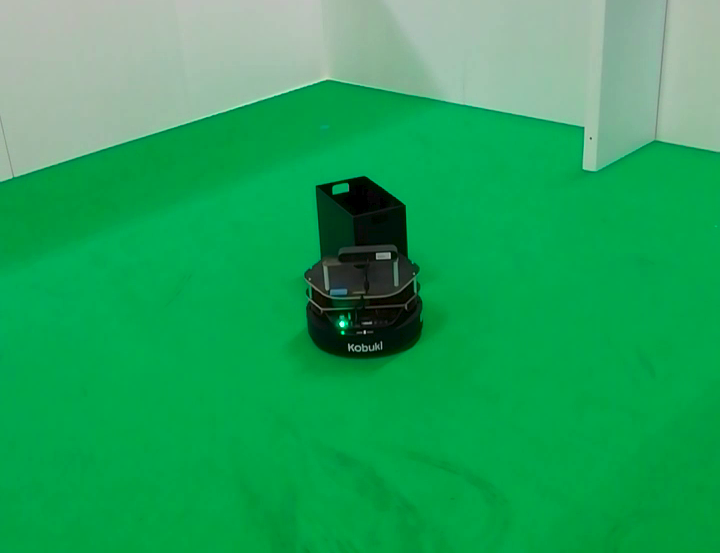
\includegraphics[width=\linewidth]{imgs/chapter5/garbageLF.png}
     \caption{Robot crashing into garbage bin}
     \label{fig:garbageLF1}
  \end{subfigure}
  \begin{subfigure}[b]{0.49\linewidth}
    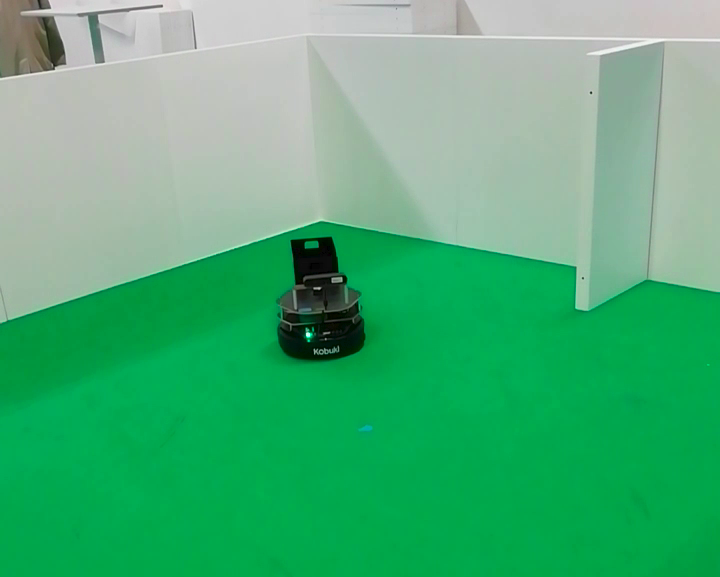
\includegraphics[width=\linewidth]{imgs/chapter5/garbageLF2.png}
    \caption{Robot pushing garbage bin}
    \label{fig:garbageLF2}
  \end{subfigure}
  \caption{Two instances of the robot's navigation with the garbage bin as an obstacle}
  \label{fig:garbageLF}
\end{figure}



\subsubsection*{FMCW radar}
Using the \ac{FMCW} radar the robot did detect it properly and went around it easily.
 Figure \ref{fig:garbageRS} shows two instances of the turtlebot avoiding the garbage bin at a safe distance.
\begin{figure}[h!]
  \centering
  \begin{subfigure}[b]{0.49\linewidth}
    \includegraphics[width=\linewidth]{imgs/chapter5/garbageRS.png}
     \caption{Robot avoiding garbage bin number 1}
     \label{fig::garbageRS1}
  \end{subfigure}
  \begin{subfigure}[b]{0.49\linewidth}
    \includegraphics[width=\linewidth]{imgs/chapter5/garbageRS2.png}
    \caption{Robot avoiding garbage bin  number 2}
    \label{fig::garbageRS2}
  \end{subfigure}
  \caption{Robot avoiding garbage bin}
  \label{fig:garbageRS}
\end{figure}

\subsubsection{Box}
\subsubsection*{LiDAR}
In the LiDAR's case the robot did not detect the low height box throughout all the course. This makes sense since the this sensor is built to detect objects that are the same height as the sensor. In other words it is optimized to detect only the horizontal plane of the 2D-\ac{LiDAR}. This failure of detection made it so the robot could not replan its course and in consequence it collided with said box. Figure \ref{fig::boxLF} shows two instances where the robot collided with the box using \ac{LiDAR} as a sensor source.

\begin{figure}[h!]
  \centering
  \begin{subfigure}[b]{0.49\linewidth}
    \includegraphics[width=\linewidth]{imgs/chapter5/boxLF.png}
     \caption{Robot collision with box number 1}
     \label{fig::boxLF1}
  \end{subfigure}
  \begin{subfigure}[b]{0.46\linewidth}
    \includegraphics[width=\linewidth]{imgs/chapter5/boxLF2.png}
    \caption{Robot collision with box number 2}
    \label{fig::boxLF2}
  \end{subfigure}
  \caption{Robot collision with box}
  \label{fig::boxLF}
\end{figure}


\subsubsection*{FMCW radar}
For this case initially the robot also did not detect the box. However by decreasing the threshold of the passthrough filter of intensity to 14 we made it so it can detect it. With this modification the robot was able to complete the test without colliding with the box. Figure \ref{fig:boxRS} shows two instances of the robot performing the course avoiding the box with the previous modification. However this change may result in the \ac{FMCW} \ac{radar} having false detections due to now having a lower level of \ac{SNR}.

\begin{figure}[ht!]
  \centering
  \begin{subfigure}[b]{0.4\linewidth}
    \includegraphics[width=\linewidth]{imgs/chapter5/boxRS.png}
     \caption{Robot avoiding box number 1}
     \label{fig:boxRS1}
  \end{subfigure}
  \begin{subfigure}[b]{0.38\linewidth}
    \includegraphics[width=\linewidth]{imgs/chapter5/boxRS2.png}
    \caption{Robot avoiding box  number 2}
    \label{fig::boxRS2}
  \end{subfigure}
  \caption{Robot avoiding box}
  \label{fig:boxRS}
\end{figure}

\subsubsection{Acrylic tube}

\subsubsection*{LiDAR}
When it comes to the Acrylic tube using the 2-D \ac{LiDAR} it falsely detected targets where there where none. This is due to the physical proprieties of the object being unsuitable for \ac{LiDAR} technology to handle. The robot in its course got stuck near the obstacle due to thinking it had crashed into it. However this was not the case and the robot did not succeed in the experiment. Figure \ref{fig:glassLF} shows two instances of the robot getting stuck in the acrylic tube.

\begin{figure}[ht!]
  \centering
  \begin{subfigure}[b]{0.49\linewidth}
    \includegraphics[width=\linewidth]{imgs/chapter5/glassLF1.png}
     \caption{Robot getting stuck acrylic tube number 1}
     \label{fig::glassLF1}
  \end{subfigure}
  \begin{subfigure}[b]{0.49\linewidth}
    \includegraphics[width=\linewidth]{imgs/chapter5/glassLF2.png}
    \caption{Robot getting stuck in acrylic tube  number 2}
    \label{fig::glassLF2}
  \end{subfigure}
  \caption{Robot getting stuck in acrylic tube}
  \label{fig:glassLF}
\end{figure}

\subsubsection*{FMCW radar}
In this case the robot was able to properly detect the tube and with it avoided it through all the course. The behavior of the robot was objectively better than the previous case since it went through all course without hitting the tube in any way. Figure \ref{fig:glassRS} shows two instances of the robot avoiding the acrylic tube.

\begin{figure}[ht!]
  \centering
  \begin{subfigure}[b]{0.49\linewidth}
    \includegraphics[width=\linewidth]{imgs/chapter5/glassRS1.png}
     \caption{Robot avoiding acrylic tube number 1}
     \label{fig::glassRS1}
  \end{subfigure}
  \begin{subfigure}[b]{0.49\linewidth}
    \includegraphics[width=\linewidth]{imgs/chapter5/glassRS2.png}
    \caption{Robot avoiding acrylic tube  number 2}
    \label{fig::glassRS2}
  \end{subfigure}
  \caption{Robot avoiding acrylic tube box}
  \label{fig:glassRS}
\end{figure}

\subsubsection{Robot  (turtlebot2) }
In this last case both the \ac{FMCW} \ac{radar} and the 2D-LIDAR performed reasonably well avoiding the obstacle with ease for all the trajectory.

\subsection{Discussion}
In this experiment we conclude that there are multiple types of obstacles that the 2-D LiDAR is unable to properly detect. This poor detection led to the robot crashing into the objects making it so the navigation task presented ended in failure. However using the \ac{FMCW} radar proved to have a better perception of all the obstacles in the experiment and with it the indoor navigation tests were concluded with success with the robot circumventing them in a safe manner.


\section{Dynamic Obstacles in controlled environment}
In the previous experiment we only dealt with static objects however in this new test we want to see how the robot handles dynamic objects in a controlled space. For that we send multiple goals  to the robot and use an additional turtlebot2 or a person to obstruct its path. In other words we have the robot trying to reach multiple goals multiple times and the dynamic obstacle will try to make more difficult by obstructing the planned paths of the robot.  The main goal of this experiment is to see if the robot can handle unstructured environments that are often the case in indoor scenarios.
\subsection{Experimental Setup}
For this test we send four goals to the robotic platform, A,B,C and D in zigzag fashion and we will place a dynamic obstacle obstructing it as shown in Figure \ref{fig:exp3}.

\begin{figure}[ht!]
\centerline{\includegraphics [width=0.5 \textwidth]{imgs/chapter5/exp3.png}}
\caption[Demonstration of the course of test]{Demonstration of the course of test, the robot will run through A-B-C-D  while  trying to avoid the dynamic obstacle obstructing its path}
\label{fig:exp3}
\end{figure}
For the dynamic obstacles we will use first person and in a second trial a a mobile robot. This obstacles will try to obstruct the path of the robot throughout the course. For this case we will only use the \ac{FMCW} \ac{radar} as an obstacle detector.


\subsection{Results}
In the following sections we show the results for the person and the mobile robot as obstacles for the experiment.
\subsubsection{Person}
Throughout all the test the robot was successfully avoided the person  only using the \ac{FMCW} \ac{radar} as an obstacle detector. Figure \ref{fig:exp3person} shows two instances of the the robot avoiding the person in the experiment.
\begin{figure}[ht!]
  \centering
  \begin{subfigure}[b]{0.49\linewidth}
    \includegraphics[width=\linewidth]{imgs/chapter5/exp3person1.png}
     \caption{Robot avoiding person number 1}
     \label{fig::exp3person1}
  \end{subfigure}
  \begin{subfigure}[b]{0.49\linewidth}
    \includegraphics[width=\linewidth]{imgs/chapter5/exp3person2.png}
    \caption{Robot avoiding person  number 2}
    \label{fig::exp3person2}
  \end{subfigure}
  \caption{Robot avoiding person }
  \label{fig:exp3person}
\end{figure}
However the robot was only able to perceive the legs of said person and not its feet. This may lead to cases where the robot shocks in the person if it is to close.

When the person got to close to the robot, it stopped completely and had to recover behaviors were activated. We conclude that the \ac{FMCW} \ac{radar} is better suited for detecting obstacles that are at least half a meter away from the robot and that are facing it directly. 
\subsubsection{Mobile Robot}
For the mobile robot case the results were similar to the previous case. The robot was able to detect and avoid the the the other robot when it is facing him.

Figure \ref{fig:exp3robot} shows two instances of the robot avoiding the dynamic robot.
\begin{figure}[ht!]
  \centering
  \begin{subfigure}[b]{0.49\linewidth}
    \includegraphics[width=\linewidth]{imgs/chapter5/exp3robot1.png}
     \caption{Robot avoiding dynamic robot 1}
     \label{fig::exp3robot1}
  \end{subfigure}
  \begin{subfigure}[b]{0.49\linewidth}
    \includegraphics[width=\linewidth]{imgs/chapter5/exp3robot2.png}
    \caption{Robot avoiding dynamic robot 2}
    \label{fig::exp3robot2}
  \end{subfigure}
  \caption{Robot avoiding dynamic robot }
  \label{fig:exp3robot}
\end{figure}

However if the robot comes from behind there is the chance of it crashing because the radar as only a small field of view of 120º.
\subsection{Discussion}
The robot was able to handle dynamic obstacles using only the \ac{FMCW} \ac{radar}, this means that it might be feasible to only use this sensor for obstacle avoidance in ever changing indoor environments.

\section {Dynamic Obstacles in uncontrolled environment}
In the following test we want to answer two things: (1) Is the robot able to avoid people that obstruct its pre planned path only using the  \ac{FMCW} radar as an obstacle detector, and (2) if in this case it is also able to clear previously obstructed spaces (by the person in this case) by ray tracing its environment. This last requirement may provide to be difficult to get since the radar point cloud is less dense than the 2D laser range finder.

\subsection{Experimental Setup}
First a map was created of the \ac{IRIS} laboratory using the package \texttt{gmapping} provided by \ac{ROS} (Fig. \ref{fig:map}). Then using the map and the package \texttt{\ac{AMCL}} we ensure that the robot localization is fairly reasonable. After that we set up the robot to do a certain navigation task.
The robot starting position and goal were set as shown in Figure \ref{fig:setup} in the \ac{IRIS} laboratory. 

\begin{figure}[ht!]
\centerline{\includegraphics [width=0.8 \textwidth]{imgs/chapter5/setup.png}}
\caption[Experimental setup]{Experimental setup showing the initial position and the goal sent to the robot. A person will be put to obstruct the path of the robot}
\label{fig:setup}
\end{figure}


In this case a single person was instructed to actively obstruct the robot's forward movement until the robot reaches its first goal. After reaching it the person is removed from the environment  and the robot is  instantaneously given a second goal which in this case is its the starting position. 

\subsection{Results}
In the following sections we will describe how the robot behaved when under different type of sensor sources. With \ac{LiDAR}, \ac{FMCW} \ac{radar} and both.

\subsubsection*{\ac{LiDAR}}
As expected the robot was able to detect and avoid the person in all 5 cases. However it should be noted that in one of this cases the robot tried to avoid it by going through an obstructed space (that was not the person) due to a missed detection. This lead to collision. The robot was also able to clear the previously obstructed spaces, getting to the starting position without avoiding past marked obstacles.

\subsection*{\ac{FMCW} \ac{radar}}
The \ac{radar} was also able to detect the obstructing person and managed to plan around it in all cases as shown in Figures \ref{fig::radarperson1}, \ref{fig::radarperson2} and \ref{fig::radarperson3}. Since the radar cloud is less dense, clearing marked obstacles was slower than in the \ac{LiDAR} case. However this did not impact the overall performance of the navigation task in a significant way since it still went to the starting position in an almost straight line (Figure \ref{fig::radarperson4}).
\begin{figure}[h!]
  \centering
  \begin{subfigure}[b]{0.49\linewidth}
    \includegraphics[width=\linewidth]{imgs/chapter5/radarperson1.png}
     \caption{Robot avoiding planning around the person blocking it}
     \label{fig::radarperson1}
  \end{subfigure}
  \begin{subfigure}[b]{0.49\linewidth}
    \includegraphics[width=\linewidth]{imgs/chapter5/radarperson2.png}
    \caption{Robot re planning around the person blocking it}
    \label{fig::radarperson2}
  \end{subfigure}
  \begin{subfigure}[b]{0.49\linewidth}
    \includegraphics[width=\linewidth]{imgs/chapter5/radarperson3.png}
    \caption{Turtlebot stopping and adjust velocity to avoid person}
    \label{fig::radarperson3}
  \end{subfigure}
  \begin{subfigure}[b]{0.49\linewidth}
    \includegraphics[width=\linewidth]{imgs/chapter5/radarperson4.png}
    \caption{Turtlebot returning to initial position in a straight line with no obstacles obstructing it}
    \label{fig::radarperson4}
  \end{subfigure}
\end{figure}
\subsection{Discussion}
 The \ac{FMCW} radar was able to perform 
obstacle avoidance of dynamic obstacles (in this case a person) that continuously obstructed its path at 5 different times in the same environment which may suggest the use of the \ac{FMCW} \ac{radar} as an alternate sensory unit over the \ac{LiDAR}.

\section{Summary}
In this chapter we proposed various experiments that try to evaluate the performance of the \ac{FMCW} \ac{radar} and the 2-D\ac{LiDAR} as obstacle detectors. In the first experiment we concluded that there are various objects in which the 2-D\ac{LiDAR} is unable to detect due to the height or proprieties of the object. However this obstacles were correctly detected by the \ac{FMCW} \ac{radar}. This means that this type of sensors  are advantagous for scenarios in which this type of obstacles are commonly used (office enviornments). We also verified how the FMCW radar handles dynamic obstacles, we succefully made the robot avoid them only using the \ac{FMCW} \ac{radar} as an obstacle detector. Finally we conducted an experiment in an unstructured enviornment with a dynamic obstacle (person). It terminated e with success in all 5 cases. WIth this we conclude that the \ac{FMCW} \ac{radar} is a good support for obstacle avoidance when it comes to use in robotic navigation procedures.

\cleardoublepage
\chapter{Towards Doppler to Enrich Obstacle Avoidance}
To ensure more safe trajectories for social indoor environments we can use velocity information from targets to generate more safe pathing for  the robot. Although we have not completed it entirely  we tried to create a software module that takes this objective in mind.

In this section we will explore the implementation of a new plugin in the ROS navigation stack based on the radar's relative radial velocity information. The plugin proposed is a map layer and can be specified by either the global or local costmap. The objective of said layer is to increase the cost values of cells based on the prediction of the motion of said obstacles provided by the radar (doppler channel). The ending result should be a better avoidance of incoming obstacles with negative relative velocity  to the robot.

\section{Layered Costmaps}
As said before the global and local costmaps used in \ac{ROS} Navigation Stack are both layered costmaps.
This means that they are composed by independent components with each one affecting the resulting master layered costmap for specific environmental contexts. For example the classic \textit{static layer} takes information from a published map topic and based on the position of the robot marks some  pre-determined obstacles while the inflation layer propagates the cost of obstacles radially.  Figure \ref{fig::layers} show some different layers for different contexts.
\begin{figure}[ht!] 
\centerline{\includegraphics [width=0.5 \textwidth]{imgs/chapter6/layers.png}}
\caption[A stack of costmap layers]{A stack of costmap layers, showcasing the different contextual
behaviors achievable with the layered costmap approach from \cite{lu2014layered}}
\label{fig::layers}
\end{figure}

The set of layers used follows a specific hierarchy that determines what order and how they overwrite the master costmap. This is an important part to take into consideration because the priority of the different layer plugins will determine the final costmap that will be used by each planner (global or local).
\section{Inflation Layer}
When it comes to define values for the costmap occupancy grid the inflation layer is usually the case in the \ac{ROS} navigation stack. By definition, inflation is the process of propagating cost values out from occupied cells that decrease with distance \cite{costmap2d}. Figure \ref{fig::inflation} shows an overview of the different values each cell can have (0 to 254) and what they mean when it comes to the robot perception. 
\begin{figure}[ht!] 
\centerline{\includegraphics [width=1.0 \textwidth]{imgs/chapter6/costmapspec.png}}
\caption[Inflation layer specifications]{Inflation layer specifications from \cite{costmap2d}}
\label{fig::inflation}
\end{figure}

All cells in the costmap further than the inscribed radius distance and closer than the inflation radius distance away from an actual obstacle is given by:
\begin{equation}
    A=253*e^{(-k * (dist - r)) }
\end{equation}
Where $k$ is the cost scaling factor  that determines how fast the decaying of the function is, $dist$ is the distance from the obstacle to the robot and finnaly $r$ is the robot radius. 
This means that cells near obstacles will have the value that will tend to 253 while cells far away from the obstacle will have values trending to 0. Note that $dist$ most be always greater than $r$ because if it isn't than it means the robot collided with said obstacle.
This inflation is only taking into account distance from the obstacle as input which means that the values of the cells will be propagated radially.

\section{Doppler Layer}
In the previous case, inflation only took into account the distance of obstacles for computing what value each cell in the costmap will have. Now we want to design a layer that not only takes into account the distance but also the relative radial velocity of the object to determine the value of cells in the costmap.
To do this we designed a layer that adjusts the cell values of the master costmap taking into account the radial velocity of said objects taken from the \ac{FMCW} \ac{radar}. Taking into account the relative  radial velocity $v_r$ the cell value of the surrounding cell's is given by:
\begin{equation} \label{eq1}
\begin{split}
cell_{cost} & = A e^{-(\frac{x^2}{2 \sigma_x^2}+\frac{y^2}{2 \sigma_y^2})} \\
 \sigma_x^2 & = cov * factor * |v_r| \\
 \sigma_y^2 & = cov \\
 x & =dist *cos(\theta)\\
 y & =dist *sin(\theta)\\
\end{split}
\end{equation}
Where $cov$ and $factor$ are parameters adjusted by the user, $\theta$ is the angle between the cell where we want to calculate its value and the direction of the velocity vector of the target object, and finally $dist$ is the distance between the two previous cells.
With this cost function we can manipulate the costmap cell values to have higher values in the directon of incoming objects. Figure \ref{fig::doppler} shows an example of the doppler layer changing the 2D master costmap taking into account the velocity and distance of the target obstacle. 

\begin{figure}[ht!] 
\centerline{\includegraphics [width=1.0 \textwidth]{imgs/chapter6/doppler.png}}
\caption[Doppler layer manipulation of the master costmap]{Example of doppler layer manipulation of the master costmap with the paramaters  A=253,factor=20 and covariance=0.1}
\label{fig::doppler}
\end{figure}
\section{Discussion}
By using the doppler layer we have concluded that the trajectory of the robot can be altered taking into consideration the relative radial velocity of the target obstacles. This may be useful for high populated indoor environments where people constantly are shifting from one place to another. This makes the robot safe from incoming obstacles and therefore is a good support for our navigation system. There are some limitations for this layer however, the first one being that the velocity resolution of the radar is limited which may produce bad results when the radial velocity of the objects is low. Another limitation is that the global costmap update is usually around 1 Hz, and alot of information may be outdated when the control loop occurs which may lead on late replanning by the global planner. For the local planner another problem is its limited dimensions do not allow the prediction of long range obstacles since it only works in the vicinity of the robot.
%\section{Summary}
%In this chapter we discussed how we can implement a new layer to manipulate the master costmap of the global and local planners. This layer inflates obstacles in the direction of their velocity. Since we have radial relative velocity of points given by the radar we can use their velocities to compute a safe path for the robot.


%\subsection{Side Tracking}

%\subsection{Target Speed Limitations}

%\section{Summary}
\cleardoublepage
\chapter{Conclusions and Future Work}


\section{Conclusion}
In this work we it was examined in detail how the \ac{FMCW} \ac{radar} and \ac{LiDAR} technology work and how they are used for certain applications. After this, it was implemented a robotic navigation platform \textbf{turtlebot2} using \ac{ROS} and \ac{TI} \ac{mmWave} devices 2D-\ac{LiDAR} that is ready to use for indoor navigation tasks.
\section{Future Work}

\cleardoublepage



%
% The bibliography
%
\bibliographystyle{IEEEtran}

%\cleardoublepage
%\phantomsection
%\addcontentsline{toc}{chapter}{Bibliography}

\bibliography{bibliography}

%
% The Appendix
%
%\appendix
%\chapter{Appendix \#A}
\section*{Matlab Code for simulation of range estimation }
\definecolor{mygreen}{RGB}{28,172,0} % color values Red, Green, Blue
\definecolor{mylilas}{RGB}{170,55,241}

\lstset{language=Matlab,%
    %basicstyle=\color{red},
    breaklines=true,%
    morekeywords={matlab2tikz},
    keywordstyle=\color{blue},%
    morekeywords=[2]{1}, keywordstyle=[2]{\color{black}},
    identifierstyle=\color{black},%
    stringstyle=\color{mylilas},
    commentstyle=\color{mygreen},%
    showstringspaces=false,%without this there will be a symbol in the places where there is a space
    numbers=left,%
    numberstyle={\tiny \color{black}},% size of the numbers
    numbersep=9pt, % this defines how far the numbers are from the text
    emph=[1]{for,end,break},emphstyle=[1]\color{red}, %some words to emphasise
    %emph=[2]{word1,word2}, emphstyle=[2]{style},    
}



\lstinputlisting{code/appendix1/range.m}
%\cleardoublepage
%\chapter{Untitled appendix \#B}
Write something here\ldots
%\cleardoublepage

\end{document}